\documentclass[cn,11pt,chinese]{elegantbook}

\title{计算机控制技术基础}
\subtitle{简单讲义}

\author{崔自强}
\institute{天津大学自动化学院}
\date{April 12, 2020}
\version{CCS-2020-Fall}
% \bioinfo{自定义}{信息}

% \extrainfo{温柔正确的人总是难以生存,因为这世界既不温柔,也不正确。—— 比企谷八幡}

% \logo{logo-blue.png}
\cover{cover.jpg}

% 本文档命令
\usepackage{array}
\newcommand{\ccr}[1]{\makecell{{\color{#1}\rule{1cm}{1cm}}}}

\begin{document}

\maketitle
\frontmatter

\chapter*{前言}
\markboth{Introduction}{前言}
《计算机控制技术基础》是自动化专业、电气工程及其自动化专业的学科基础必修课。本课程是一门理论与实践结合紧密的课程,其中,涵盖或涉及了电路基础、模拟电子技术基础、数字电子技术基础、自动控制原理、微型计算机原理及应用等课程的相关内容。通过本课程的学习,使同学在应用层面综合理解以往课程,掌握构建计算机控制系统的基本方法。具体地讲,本课程将从软硬件结合的角度使学生掌握过程通道的结构特点及设计方法、数据通信基础知识、数据处理及抗干扰技术和数据总线与网络知识。

\begin{enumerate}
  \item 本讲义作为历年备课积累之用,供本校有需要的教师、同学使用;
  \item 讲义本身无法代替课堂教学及学习笔记;
  \item 讲内容难免有误,请老师和同学不吝指正。编者会在每一个新学期进行更新和补足。
\end{enumerate}
\vskip 1.5cm

\begin{flushright}
崔自强于天津大学\\cuiziqiang@tju.edu.cn\\
2015年10月20日
\end{flushright}



\tableofcontents
%\listofchanges

\mainmatter


\graphicspath{{figure/}{fig/}}

\chapter{绪论}



计算机控制技术基础与多门课程相关联,例如:数电、模电、单片机、微机原理、计算机接口技术、自动控制、电机学、运动控制、过程控制等。与其他课程的关系体现在以下几方面:

\begin{itemize}
  \item
输入/输出过程通道:模电、数电、计算机接口技术等;
  \item
计算机/CPU:单片机、微机原理、PLC、DSP、ARM、FPGA等;
  \item
方法及应用:自动控制、运动控制、过程控制、PID、电机学等;
  \item
总线技术:网络技术、USB总线、工业现场总线等。
\end{itemize}




\section{计算机控制系统基本概念}




通俗地讲,利用\textbf{计算机参与控制}的系统称为计算机控制系统。


\begin{table}[h]
  \centering
\begin{tabular}{|c|c|}
  \hline
  % after \\: \hline or \cline{col1-col2} \cline{col3-col4} ...
  模拟控制系统 & 计算机控制系统 \\ \hline
  难以实现复杂规律的调节控制 & 实时数据处理 \\
  不易实现集中监视和操作 & 实时监督决策 \\
  控制方案的更改比较困难 & 实时控制输出 \\
  \hline
\end{tabular}
  \caption{模拟控制与计算机控制系统的对比}\label{tab:1.1}
\end{table}








\section{计算机控制系统的组成}

计算机控制系统由控制计算机和被控对象组成,控制计算机包括硬件和软件两部分:

\begin{itemize}
  \item 硬件:
  \begin{enumerate}
    \item 主机
    中央处理器(CPU)、存储器和接口组成的主机是计算机控制系统的核心。
    \item 过程输入输出设备,
   是主机与被控对象之间的接口,包括模拟量输入输出设备、数字量输入输出设备等。
    \item 人机接口设备
    包括显示器、键盘和打印机等,作用:显示生产过程的状况,供操作员对生产过程发出操作命令,显示操作控制的结果。
    \item 通信设备
  \end{enumerate}


  \item 软件:
  \begin{enumerate}
    \item 系统软件
    可分为通用和专用两类。通用软件指一般计算机使用的软件,如:Windows、VB和Oracle等;专用软件指控制计算机特有的软件,如组态软件。
    \item 应用软件
   是针对某个生产过程编制或生成的专用控制软件。(输入输出、控制算法、人机接口,打印制表)
    \item 管理软件
    实现控制和管理的集成,包括:控制管理、操作管理、经营管理和决策管理等。
  \end{enumerate}

\end{itemize}








\section{计算机控制系统的信号流程}

如图\ref{fig_1_01}所示,计算机控制系统中涉及到以下几种信号:

\begin{figure}[h]
  \centering
  % Requires \usepackage{graphicx}
  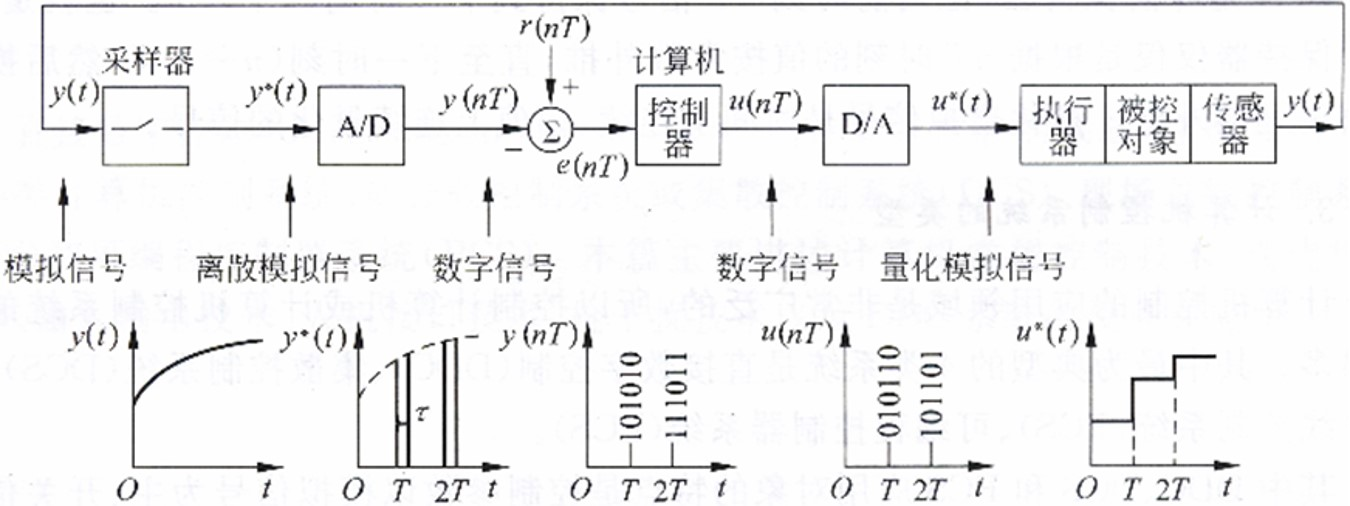
\includegraphics[width=0.8\textwidth]{fig_1_01.jpg}\\
  \caption{计算机控制系统的信号流程}\label{fig_1_01}
\end{figure}


\begin{description}
  \item[模拟信号] 时间与幅值上均连续,如: y(t)、u(t)
  \item[离散模拟信号] 时间离散,幅值连续,如:y*(t)
  \item[数字信号] 时间离散,幅值为数字量,如:y(nT)、u(nT)
  \item[量化模拟信号] 时间连续,幅值为连续量化的信号,如: u*(t)
\end{description}


\section{计算机控制系统分类}

\subsection{按照计算机参与控制的方式}

\begin{itemize}
  \item 开环控制;
  \item 闭环控制。
\end{itemize}

\subsection{按照系统采用的控制规律}


\begin{itemize}
  \item 顺序控制;
  \item 常规控制(PID控制);
  \item 高级控制算法(先进控制、最优控制、自适应控制、预测控制、模糊控制)
  \item 智能控制
\end{itemize}

\subsection{按照计算机应用于工业控制的发展历程及结构特点}



\begin{itemize}
  \item 数据采集系统(DAS:Data Acquisition System)

  \item 操作指导系统(DPS:Data Process System)

  \item 直接数字控制(DDC:Direct Digital Control)

  \item 监督控制系统(SCC:Supervisory Computer Control)

  \item 集散控制系统(DCS:Distributed Control System)

  \item 现场总线控制系统(FCS:Fieldbus Control System )

\end{itemize}

DCS:集散控制系统、分布式、分散型控制;“操作站+工作站+现场仪表”

\begin{itemize}
  \item 计算机价格的下降规律(Intel的摩尔定律:每隔18-24月,计算机性能提升1倍;单位成本下降1/2);
  \item 分散风险;
  \item 构成灵活、积木式、方便替换、维护方便。
\end{itemize}



FCS:现场总线控制系统;随着智能仪表的发展,催生出“工作站+现场总线智能仪表”的系统结构。

\section{本章要点总结}

\begin{enumerate}
  \item 计算机控制系统的概念
  \item 计算机控制系统的组成

  \item 了解计算机控制系统的信号流程
  \item 计算机控制系统的主要类型和各自特点

\end{enumerate}


\setcounter{chapter}{1}
\chapter[]{过程通道技术}


\section{概述}

过程通道是计算机和生产过程之间设置的信息传送和转换的连接通道,如图\ref{fig_2_01}所示。


\begin{figure}[h]
  \centering
  % Requires \usepackage{graphicx}
  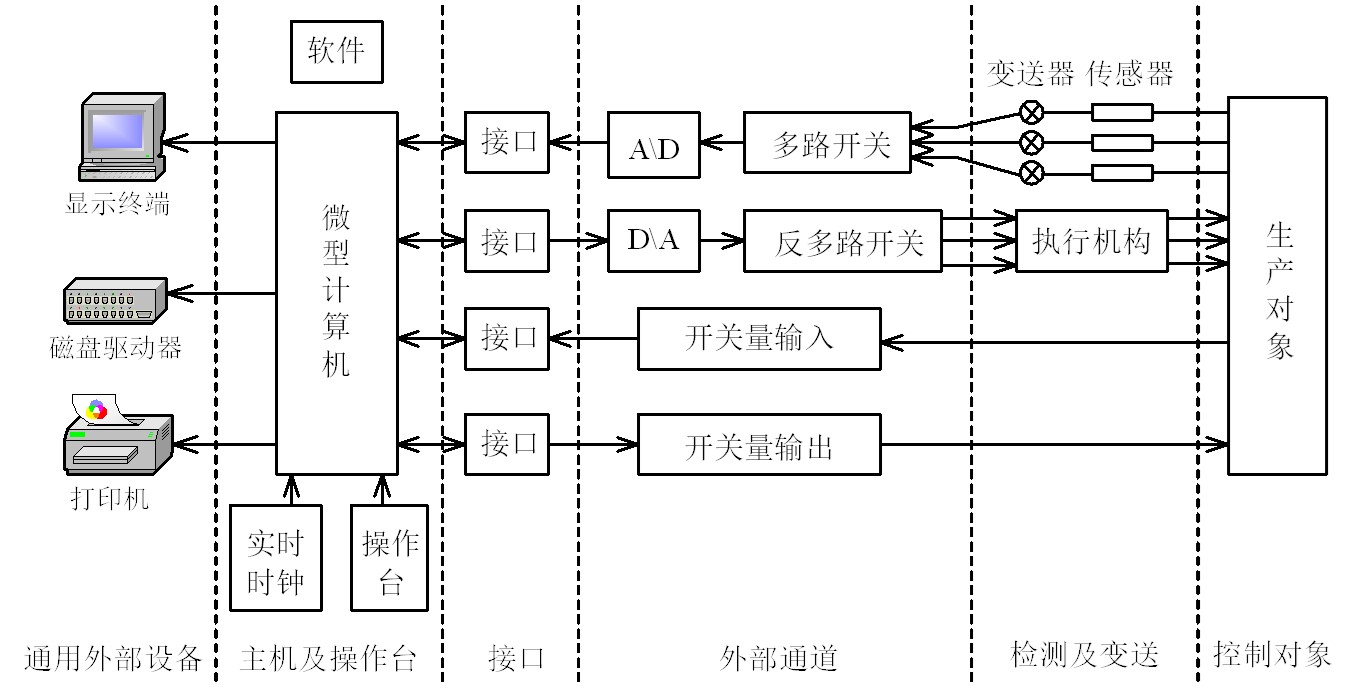
\includegraphics[width=0.8\textwidth]{fig_2_01}\\
  \caption{过程通道}\label{fig_2_01}
\end{figure}



过程通道包括:
\begin{table}[h]
  \centering
  \begin{tabular}{|c|c|}
  \hline
  % after \\: \hline or \cline{col1-col2} \cline{col3-col4} ...
  检测通道/输入通道 & 控制通道/输出通道 \\  \hline

     数字量输入通道& 数字量输出通道\\

     脉冲量输入通道& 脉冲量输出通道\\

     模拟量输入通道& 模拟量输出通道\\  \hline
\end{tabular}

  \caption{过程通道}\label{tab:2.1}
\end{table}

其中,脉冲量有时也作为数字量处理。





\section{通道接口技术}




\subsection{通道地址译码技术}

\begin{remark}
  为什么需要编址和译码?

  以通道接口的观点看,CPU与输入/输出通道的关系是一对多,而非一对一。如果要对其中某一个通道进行输入/输出操作,就需要给每个通道接口设定一个地址,即为编址。当CPU需要操作一个通道接口时,就可利用CPU总线输出一个该地址,配合数字组合逻辑电路,产生一个使能信号(Enable)或称选通信号(Select)使该地址对应的通道接口可与CPU进行数据的交换。
\end{remark}

\subsubsection{编址方式}

\begin{itemize}
  \item 存储器统一编址方式(WR、RD)

存储器指令丰富,使用灵活,程序设计方便;占用了存储空间地址,指令执行时间较长,难以区分I/O操作。

  \item I/O接口编址方式(MREQ、IORQ配合WR和RD或IOW、IOR)

I/O指令简单,执行时间短,硬件设计简单,程序设计清晰;输入输出数据必须经过累加器A。

\end{itemize}



\subsubsection{地址译码}

\begin{enumerate}
  \item 译码器译码
  \begin{itemize}
    \item 适合连续多个地址的译码电路设计
    \item 常用的译码器芯片:3-8译码器74LS138;74LS154,是4-16译码器


    \item \textbf{3-8译码器举例}
  \end{itemize}



  \item 通用阵列逻辑(GAL:Generic Array Logic)器件译码:由译码器构成的译码电路虽能很好地完成译码功能。但都需要非止一个器件来构成译码电路。在实际应用中需要较大的安装空间和较多种类的产品备件.这将影响最终产品的成本、可靠性及可维护性。
\begin{itemize}
  \item 具有可编程的与门及或门阵列;
  \item 可定义每个输出引脚的结构和功能;
  \item GAL器件可在线电擦写、编程,数据保持时间在10年以上;
  \item GAL器件有较高的响应速度,与TTL兼容;
  \item GAL器件具有可编程的保密位,防止非法读取和复制。
  \item 常用GAL器件:GAL16v8、GAL20v8

\end{itemize}

\end{enumerate}


\textbf{例:3-8译码器举例}: 74LS138译码器的管脚图及真值表见下图:

\begin{figure}[h]
  \centering
  % Requires \usepackage{graphicx}
  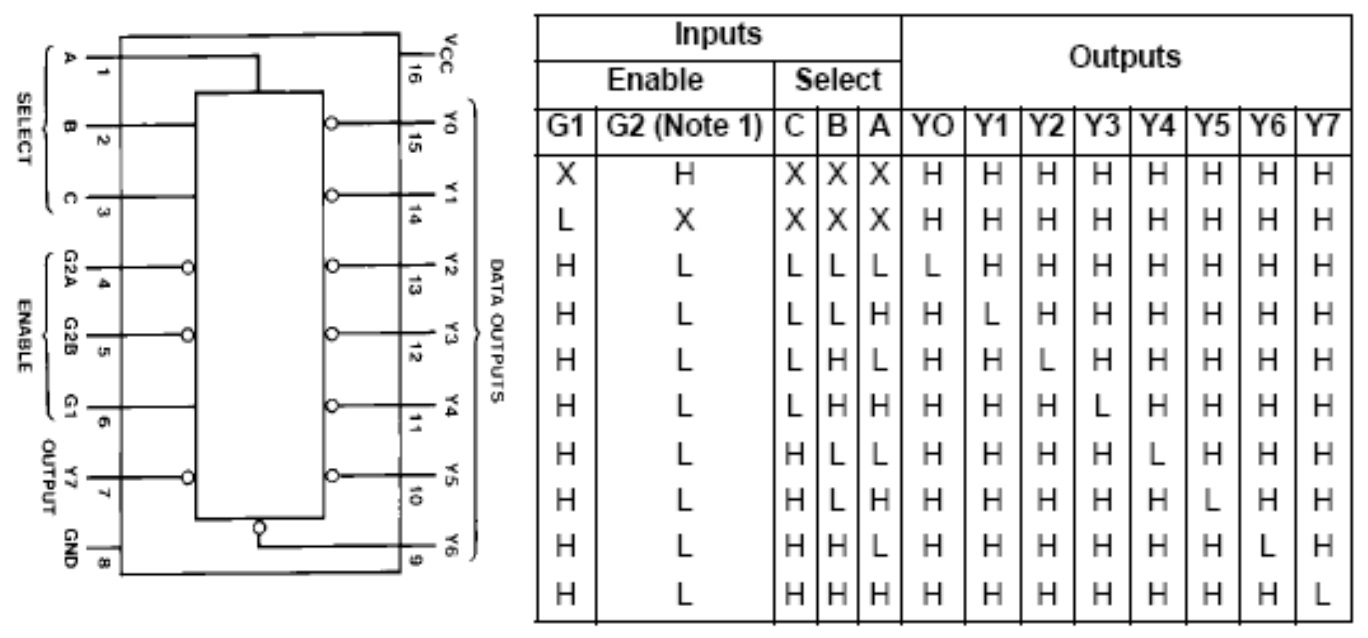
\includegraphics[width=0.5\textwidth]{74ls138}\\
  \caption{74LS138译码器}\label{fig:138_1}
\end{figure}

掌握一种数字逻辑电路芯片的关键是读懂其真值表。首先,了解一些术语的含义,参见下表。其次,解读其使用方法。例如,要想使74LS138工作,必然要求满足G1=H、G2=L,否则不管C/B/A为何值,输出Y0-Y7都一直为H。当满足G1=H、G2=L 后,输出Y0-Y7会随着C/B/A 的变化。最后,根据输入/输出的关系,设定Y0-Y7的地址,应是水到渠成。

\begin{table}[h]
  \centering
\begin{tabular}{|l|l|}
  \hline
  % after \\: \hline or \cline{col1-col2} \cline{col3-col4} ...
  H: 高电平 & L: 低电平 \\
  X: Don't care/无作用 & Z: 高阻态 \\
  Enable: 使能 & Select:选择/选通 \\
  \hline
\end{tabular}
  \caption{真值表常用术语}\label{tab:2.2}
\end{table}


以下图为例,考虑:
\begin{enumerate}
  \item 要求Y0-Y7能够在地址总线输出2E0H-2E7H时分别实现使能,应当如何连接?
  \item 或者,反过来,当采用如图的连接时,Y0-Y7分别对应什么地址?
\end{enumerate}


\begin{figure}[h]
  \centering
  % Requires \usepackage{graphicx}
  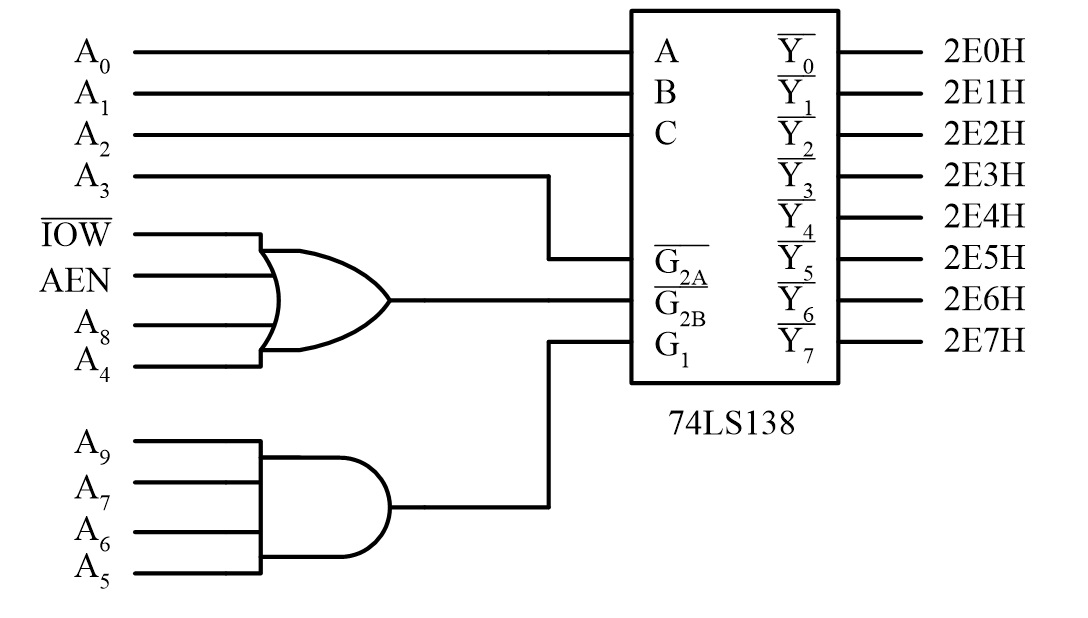
\includegraphics[width=0.5\textwidth]{74ls138_2}\\
  \caption{74LS138译码器使用举例}\label{fig:138_2}
\end{figure}




需要的知识:
\begin{itemize}
  \item A0-A9共10位,为地址总线
  \item AEN为地址总线使能,使能时为低电平
  \item $\overline{IOW}$为写IO功能,使能时为低电平。
  \item 74LS138的管脚同理
  \item 与门:所有输入均为1,输出才为1;或者说,要满足输出为1,所有输入必为1
  \item 或门:……
\end{itemize}

到此为止,以大家的智商,应该可以解决以上两个问题。进一步,应该形成一个解决问题的方法。

\begin{enumerate}
  \item 将地址写为二进制形式,例如:$2E0H-2E7H=01,1110,0XXXB$;
  \item 将C/B/A对应A2/A1/A0(注意:仅连续译码时才是这种连接);
  \item 将应为0的信号(包括A3-A9,${AEN}$,$\overline{IOW}$)与$\overline{G2A}$或$\overline{G2B}$或对应的四输入或门相连。
  \item 将应为1的信号与G1或对应的四输入与门相连。
\end{enumerate}

\begin{remark}
  74LS138芯片是为实现连续地址译码设计的芯片,但也可以实现非连续地址的译码。如何实现,可参见数电课程中的相关知识,通过增加相应的数字电路实现。
\end{remark}



\subsection{总线接口常用芯片}


在应用系统中,几乎所有系统扩展的外围芯片都是通过总线与CPU连接的,但是:


\begin{itemize}
  \item  总线的数目是有限的;

  \item 外围芯片工作时有一个输入电流,不工作时也有漏电流存在,因此总线只能带动一定数量的电路;

  \item 对于多电压系统,不同电平标准芯片的连接也需要电平的匹配;

\end{itemize}


\begin{remark}

一.TTL

      TTL集成电路的主要型式为晶体管-晶体管逻辑门(transistor-transistor logic gate),TTL大部分都采用5V电源。

      1.输出高电平Uoh和输出低电平Uol

      $U_{oh}\ge 2.4~V$, $U_{ol}\le 0.4~V$

      2.输入高电平和输入低电平

      $U_{ih}\ge 2.0~V$,$U_{il}\le 0.8~V$

二.CMOS

      CMOS电路是电压控制器件,输入电阻极大,对于干扰信号十分敏感,因此不用的输入端不应开路,接到地或者电源上。CMOS 电路的优点是噪声容限较宽,静态功耗很小。

1.输出高电平Uoh和输出低电平Uol

$Uoh\approx VCC$,$Uol\approx GND$

2.输入高电平Uoh和输入低电平Uol

$U_{ih}\ge 0.7~VCC$,$U_{il}\le 0.2~VCC$

(VCC为电源电压,GND为地)

\end{remark}

\subsubsection{锁存器}

74LS574、74LS573\newline

\begin{figure}[h]
  \centering
  % Requires \usepackage{graphicx}
  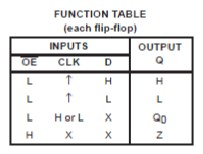
\includegraphics[height=0.2\textwidth]{fig_2_574}(a)
  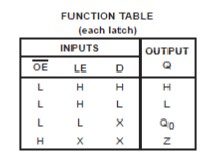
\includegraphics[height=0.19\textwidth]{fig_2_573}(b)\\
  \caption{74LS574(a)/573(b)锁存器的真值表}\label{fig:fig_2_574}
\end{figure}



\begin{remark}
锁存器可将数据锁定在其输出端,使数据稳定下来保持一段时间不变化,直到CPU用新的数据将其替换,用于实现数据从CPU到外设的传送。
\end{remark}

\subsubsection{缓冲器}

74LS244、74LS245\newline


\begin{figure}[h]
  \centering
  % Requires \usepackage{graphicx}
  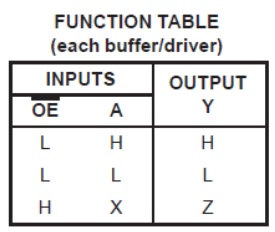
\includegraphics[height=0.2\textwidth]{fig_2_244}(a)
  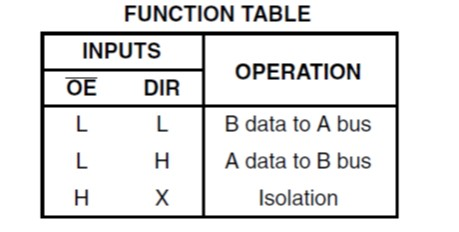
\includegraphics[height=0.17\textwidth]{fig_2_245}(b)\\
  \caption{74LS244(a)/245(b)缓冲器的真值表}\label{fig:fig_2_244}
\end{figure}



\begin{remark}
缓冲器可以使高速工作的CPU与慢速工作的外设 协调工作,实现数据从外设到CPU的传送。由于缓冲器的输出接在数据总线上,故必须具有三态输出功能。为什么?


三态输出门具有‘1’,‘0’,‘Z’三种输出状态。其中,高阻态‘Z’用于器件间信号隔离,当需要隔离的时候就置输出为‘Z’ 态,那么其他器件的信号就不会对本器件内数据构成影响,例如一条数据总线上连接有两片缓冲器(甲和乙),甲在输出给CPU时,乙就要置输出为‘Z’态,否则甲/乙的输出电平会在数据总线上产生冲突。

\end{remark}



\section{数字量输入通道}

\subsection{数字量输入通道的结构}



什么芯片可实现这里的输入缓冲?
\begin{figure}[h]
  \centering
  % Requires \usepackage{graphicx}
  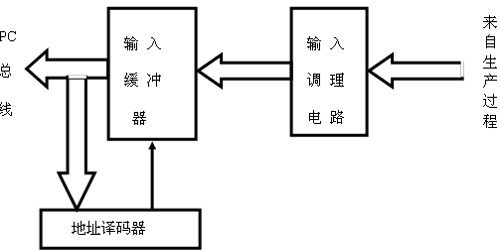
\includegraphics[width=0.5\textwidth]{fig_2_02}\\
  \caption{数字量输入通道的结构}\label{fig_2_02}
\end{figure}


\subsection{数字量输入调理电路}
\textbf{信号调理}:将现场输入的信号经转换、保护、滤波、隔离等措施转换成计算机能够接收的逻辑信号。可能引入瞬时的高压、过电压、接触抖动等现象。开关量(数字量)的种类:
\begin{itemize}
  \item 按类型分有电平式和触点式两种
  \begin{itemize}
    \item 电平式为高电平或低电平
    \item 触点式为触点闭合或触点断开
  \end{itemize}
  \item 按电源分有有源和无源两种
  \begin{itemize}
    \item 有源即直接提供高、低电平

    \item 无源即提供物理触点,或感应器件

  \end{itemize}

\end{itemize}


\subsubsection{对抖动的调理}

两种常用的方法,如图\ref{fig_2_03}所示。
\begin{enumerate}
  \item 利用RC滤波电路
  \item 利用R-S双稳态触发电路
\end{enumerate}



\begin{figure}[h]
  \centering
  % Requires \usepackage{graphicx}
  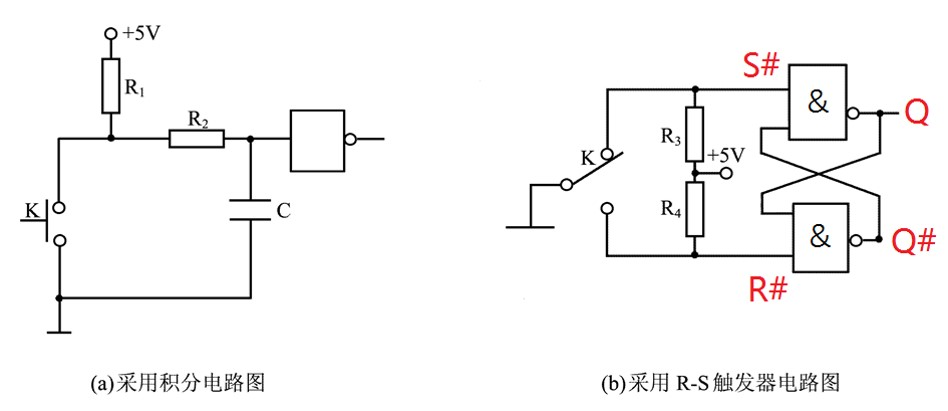
\includegraphics[width=0.6\textwidth]{fig_2_03}\\
  \caption{消抖电路}\label{fig_2_03}
\end{figure}

\begin{remark}
  R-S双稳态触发电路如何消抖?
\begin{itemize}
  \item 开关K可以使$S\#$和$R\#$处于何种状态;
  \item R-S双稳态触发电路的性质,参见图\ref{fig_2_rs}(a);
  \item 考虑正常情况和非正常(按键K出现抖动)情况下,电路的输出如何响应。
\end{itemize}
\end{remark}

\begin{figure}[h]
  \centering
  % Requires \usepackage{graphicx}
  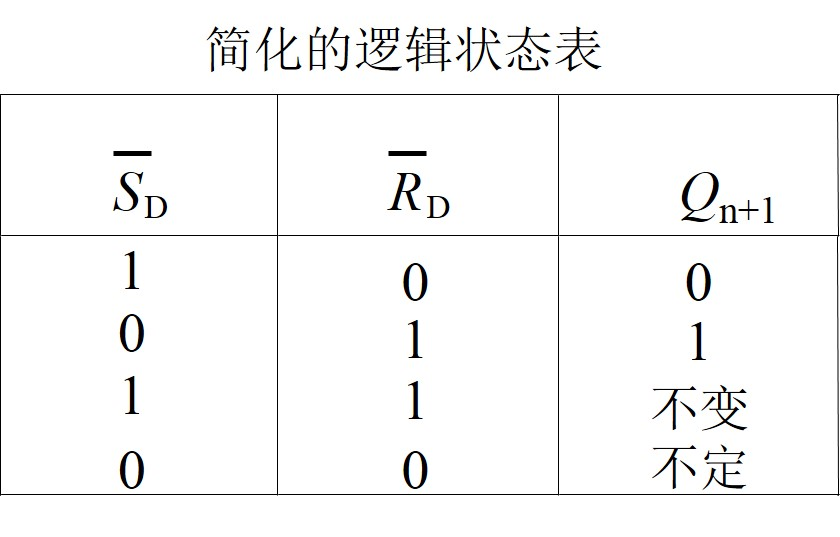
\includegraphics[width=0.35\textwidth]{fig_2_rsa}(a)
  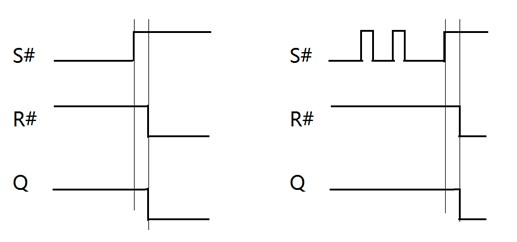
\includegraphics[width=0.45\textwidth]{fig_2_rs}(b)\\
  \caption{双稳态触发电路消抖的原理}\label{fig_2_rs}
\end{figure}

\subsubsection{保护}

数字量输入通道常用的保护电路,如图\ref{fig_2_04}所示。理解各元件的保护功能,可以从各元件的伏安特性曲线入手。常见的电阻是典型的线性元件,满足$U=IR$;各种二极管、三极管和压敏电阻则是非线性元件,合理的使用可起到保护主要电路的作用。


\begin{figure}[h]
  \centering
  % Requires \usepackage{graphicx}
  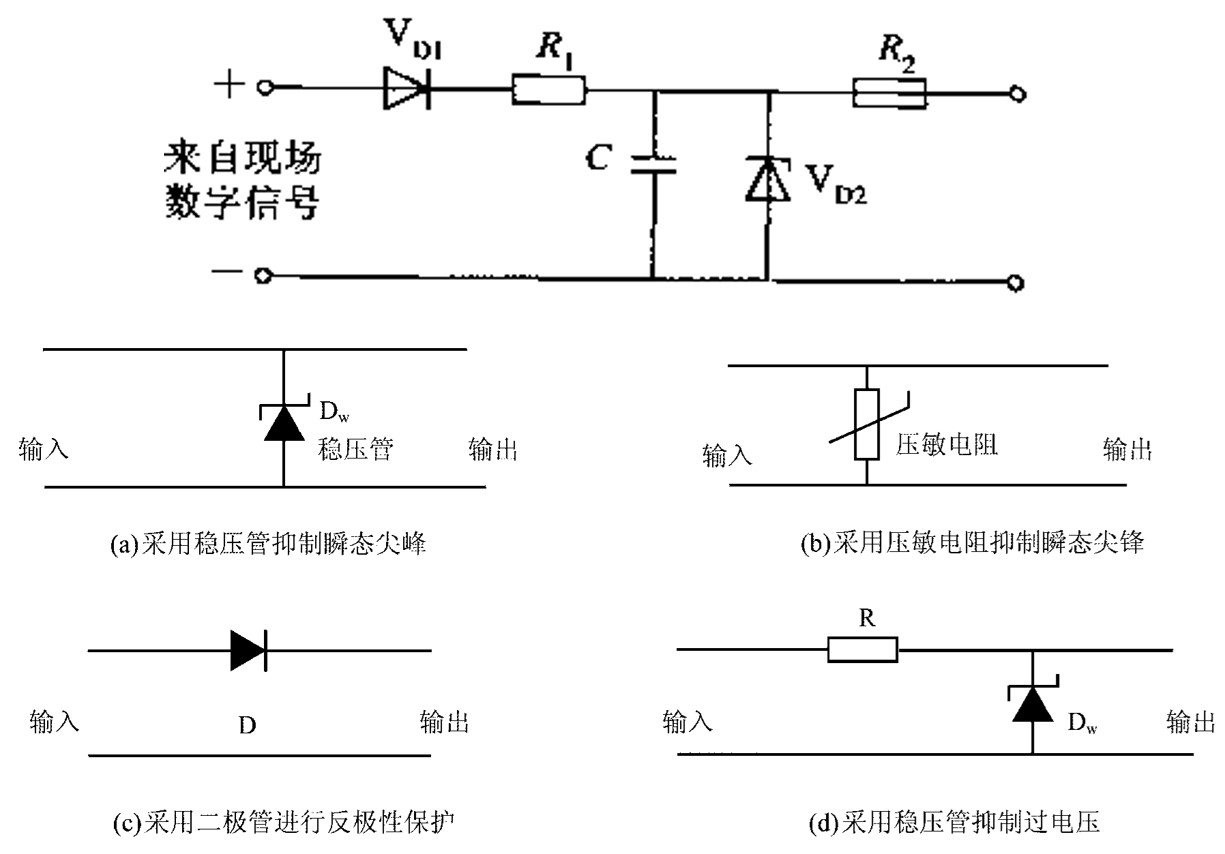
\includegraphics[width=0.6\textwidth]{fig_2_04}
  \caption{保护电路}\label{fig_2_04}
\end{figure}



以稳压二极管为例,其伏安特性如图\ref{fig_2_04a}所示。稳压二极管的特点就是被反向击穿后,其两端的电压基本保持不变。这样,当把稳压管接入电路以后,若由于电源电压发生波动,或其它原因造成电路中各点电压变动时,负载两端的电压将基本保持不变。

\begin{figure}[h]
  \centering
  % Requires \usepackage{graphicx}
  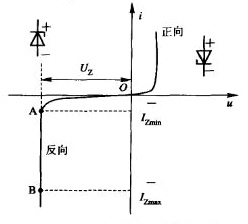
\includegraphics[width=0.3\textwidth]{fig_2_04a}
  \caption{稳压管的伏安特性}\label{fig_2_04a}
\end{figure}


\subsubsection{隔离}

在工业现场获取的开关量或数字量的信号电平往往高于计算机系统的逻辑电平,即使输入数字量电压本身不高,也可能从现场引入意外的高压信号,因此必须采取电隔离措施,以保障系统安全。


光电耦合器,简称光耦,是一种常用且非常有效的电隔离手段,由于它价格低廉,可靠性好,被广泛地应用于现场输入设备与计算机系统之间的隔离保护。光电耦合器是把发光器件和光敏器件组装在一起,通过光实现耦合构成‘电-光’和‘光-电’转换的器件,如图\ref{fig_2_05a}(a)所示为其原理图。


\begin{figure}[h]
  \centering
  % Requires \usepackage{graphicx}
  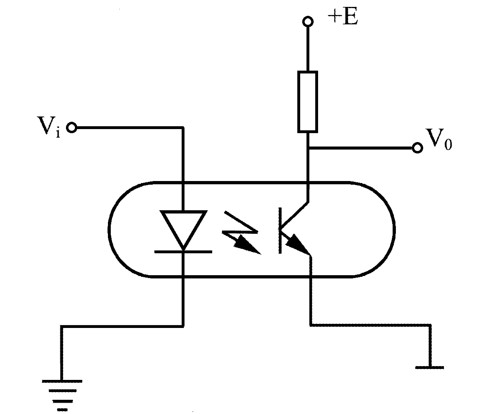
\includegraphics[width=0.2\textwidth]{fig_2_05a}(a)
  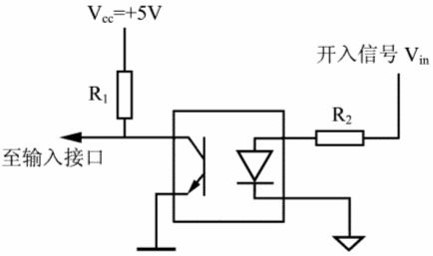
\includegraphics[width=0.3\textwidth]{fig_2_05b}(a)
    \caption{光电耦合器}\label{fig_2_05a}
\end{figure}


当电信号送入光耦输入端时,发光二极管发光,光敏器件受到光照后产生电流,ce导通;反之,ce不导通。对于数字量,输入为低电平‘0’时,光敏三极管截止,输出为高电平;反之,输出为低电平。




\begin{description}
  \item[常开] —NO(normal open)通常情况下是断开状态,即线圈未得电的情况下断开的。在常态(不通电)的情况下处于断开状态的触点叫常开触点。

  \item[常闭] —NC(normal close)通常情况下是关合状态,即线圈未得电的情况下闭合的。在常态(不通电、无电流流过)的情况下处于闭合状态的触点叫常闭触点。


\end{description}




\section{数字量输出通道}

\subsection{数字量输出通道的结构}

\begin{figure}[h]
  \centering
  % Requires \usepackage{graphicx}
  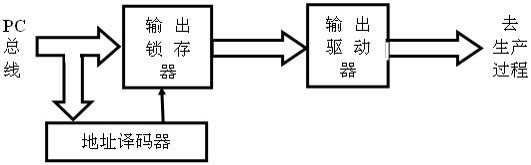
\includegraphics[width=0.5\textwidth]{fig_2_05}
  \caption{数字量输出通道的结构}\label{fig_2_05}
\end{figure}


\subsection{数字量输出调理电路}

数字量输出的信号调理主要是进行功率放大,使控制信号具有足够的功率去驱动执行机构或其它负载。

\begin{enumerate}
  \item 小功率直流驱动电路 (几十毫安级 )
\begin{figure}[h]
  \centering
  % Requires \usepackage{graphicx}
  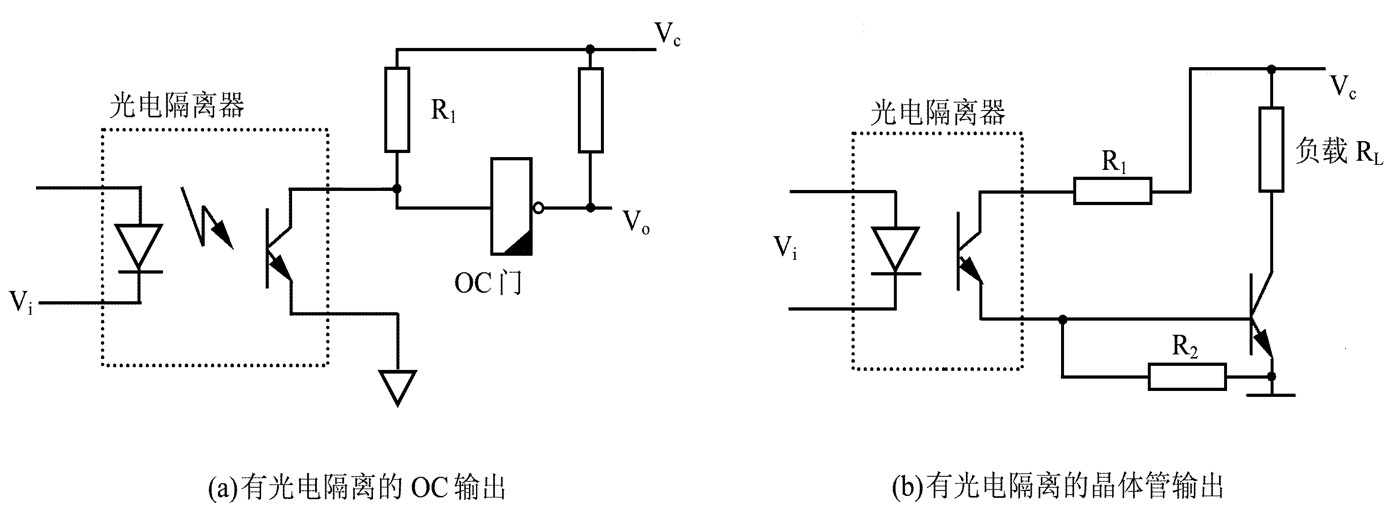
\includegraphics[width=0.6\textwidth]{fig_2_05c}
  \caption{十毫安级直流驱动电路}\label{fig_2_05c}
\end{figure}


\begin{remark}
什么是OC门?

OC门,又称集电极开路门,Open Collector,
还有OD门(Open Drain,漏极开路门,对场效应管而言)。实际使用中,有时需要两个或两个以上与非门的输出端连接在同一条导线上,将这些与非门上的数据(状态电平)用同一条导线输送出去。因此,需要一种新的与非门电路--OC门来实现“线与逻辑”。

\end{remark}

\begin{remark}
NPN与PNP三极管?


\end{remark}


  \item 继电器输出技术

      继电器经常用于计算机控制系统中的开关量输出功率放大,即利用继电器作为计算机输出的第一级执行机构,通过继电器的触点控制大功率接触器的通断,从而完成从直流低压到交流高压,从小功率到大功率的转换。

\begin{figure}[h]
  \centering
  % Requires \usepackage{graphicx}
  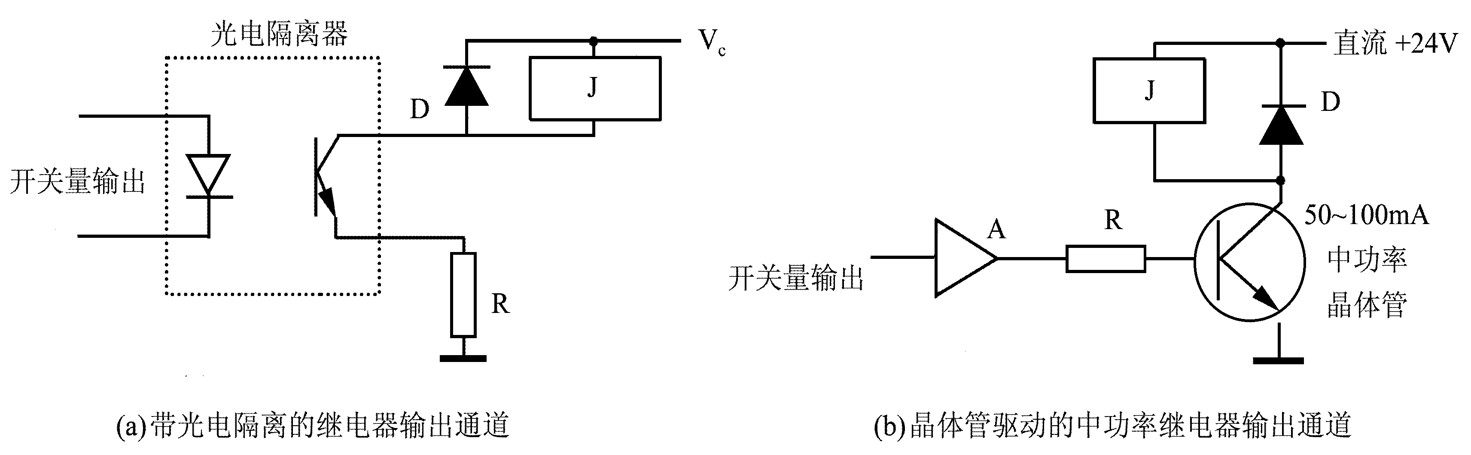
\includegraphics[width=0.6\textwidth]{fig_2_05d}
  \caption{继电器驱动}\label{fig_2_05d}
\end{figure}

\begin{remark}
二极管D的作用?续流,防止晶体管断开后线圈中的电流冲击晶体管而导致损坏。
\end{remark}

  \item 大功率交流驱动电路

      对于交流供电的负载,其开关量的输出控制可用固态继电器(Solid State Relay,SSR)来实现。


\begin{figure}[h]
  \centering
  % Requires \usepackage{graphicx}
  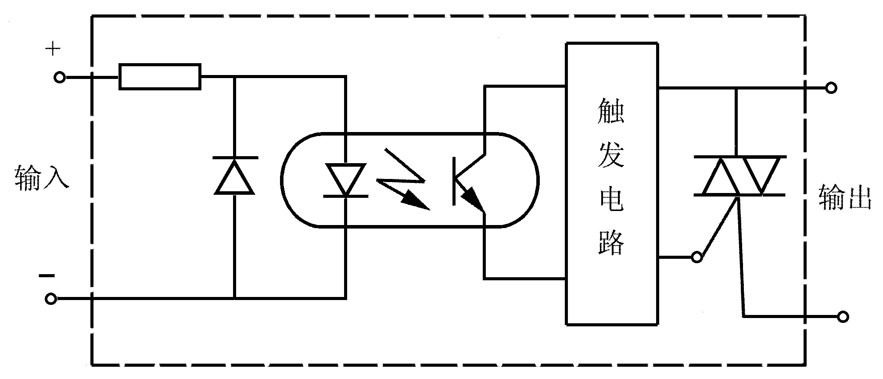
\includegraphics[height=0.1\textheight]{fig_2_05e}
  \caption{固态继电器内部结构示意图}\label{fig_2_05e}
\end{figure}


\begin{figure}[h]
  \centering
  % Requires \usepackage{graphicx}
  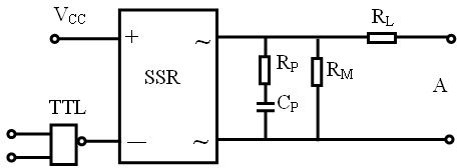
\includegraphics[height=0.1\textheight]{fig_2_05f}
  \caption{TTL驱动固态继电器}\label{fig_2_05f}
\end{figure}


\begin{figure}[h]
  \centering
  % Requires \usepackage{graphicx}
  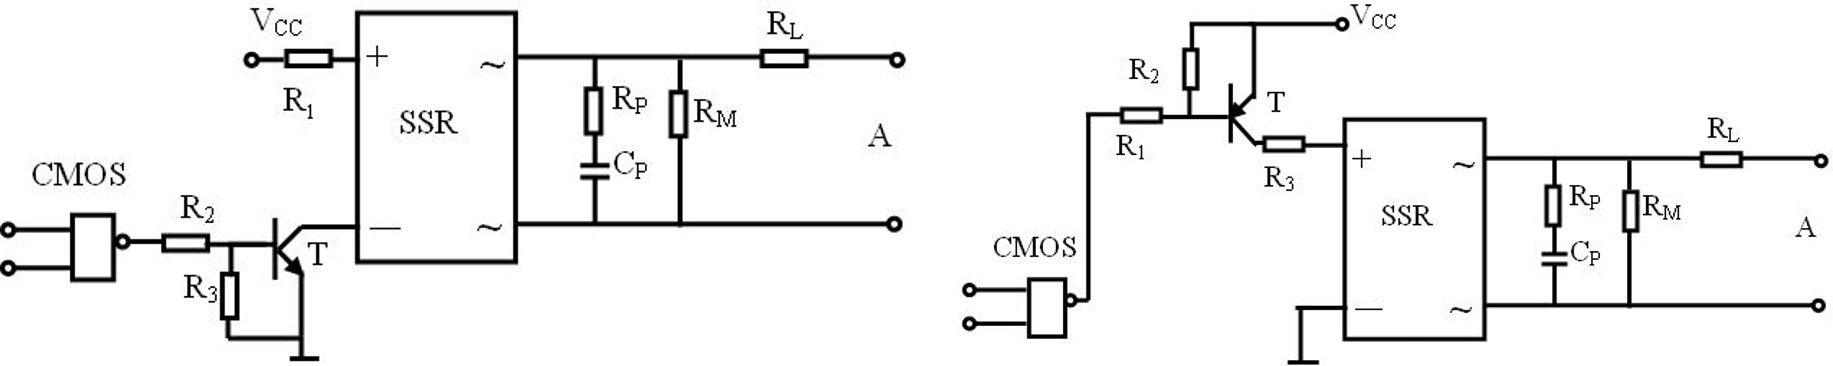
\includegraphics[height=0.1\textheight]{fig_2_05h}
  \caption{CMOS驱动固态继电器}\label{fig_2_05h}
\end{figure}

\begin{itemize}

  \item 分类:直流型(DC-SSR)节点通直流电;交流型(AC-SSR)节点通交流电。

  \item 特点:输入功率小、可靠性高、低噪声、能承受的浪涌电流大、对电源电压适应能力强(交流型对负载30V—220V)、抗扰能力强。


  \item 注意:
  \begin{itemize}
    \item 存在通态压降($<2V$);

    \item 电流负载能力随温度升高而下降,选用时留余量;

    \item SSR过载能力差,当感性负载时需加压敏电阻保护,电压选1.6~1.9 倍电源电压;
\item 输出负载短路会造成SSR损坏。

  \end{itemize}
\end{itemize}



\end{enumerate}


\begin{remark}
PNP与NPN型传感器是利用三极管的饱和和截止,输出两种状态,属于开关型传感器;其输出信号是截然相反的,即高电平和低电平。PNP与NPN型传感器一般有三条引出线,即电源线VCC、0V线,out信号输出线。在有信号触发时,NPN输出是低电平0,PNP输出的是高电平1。PNP与NPN型传感器(开关型)分为六类:
\begin{enumerate}
  \item
NPN-NO(常开型):在没有信号触发时,输出线是悬空的,就是0V线和out线断开。有信号触发时,发出与0V相同的电压,也就是out线和0V线连接,输出输出低电平0V。
  \item
NPN-NC(常闭型):在没有信号触发时,发出与0V线相同的电压,也就是out线和0V线连接,输出低电平0V。当有信号触发后,输出线是悬空的,就是0V线和out线断开。
  \item
NPN-NC+NO(常开、常闭共有型):多出一个输出线OUT,根据需要取舍。
  \item
PNP-NO(常开型):在没有信号触发时,输出线是悬空的,就是VCC电源线和out线断开。有信号触发时,发出与VCC电源线相同的电压,也就是out线和电源线VCC连接,输出高电平VCC。
  \item
PNP-NC(常闭型):在没有信号触发时,发出与VCC电源线相同的电压,也就是out线和电源线VCC连接,输出高电平VCC。当有信号触发后,输出线是悬空的,就是VCC电源线和out线断开。
  \item
PNP-NC+NO(常开、常闭共有型)其实就是多出一个输出线OUT,根据需要取舍。
\end{enumerate}

在使用时,应注意:

\begin{itemize}
  \item 如果直流电压具有V+公共端,则需要NPN输出传感器;
  \item 如果直流电压具有V-公共端,则需要PNP输出传感器。
\end{itemize}

\end{remark}

\begin{figure}[h]
  \centering
  % Requires \usepackage{graphicx}
  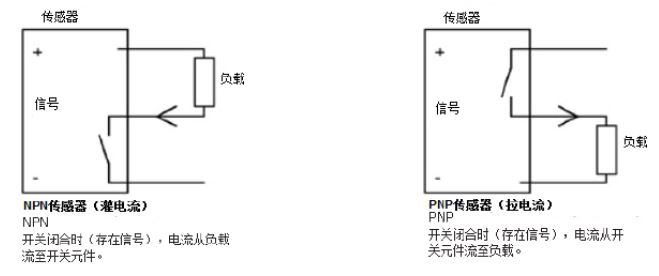
\includegraphics[width=0.6\textwidth]{fig_2_05i.jpg}
  \caption{NPN与PNP传感器}\label{fig_2_05i}
\end{figure}

\section{模拟量输入通道}

\subsection{模拟量输入通道的结构}

对于高速系统.特别是需要同时得到描述系统性能各项数据的系统,可采用图\ref{fig_2_06}所示并行转换结构。其特点是速度快、工作可靠,即使某一通路有故障,也不会影响其他通路正常工作。


\begin{figure}[h]
  \centering
  % Requires \usepackage{graphicx}
  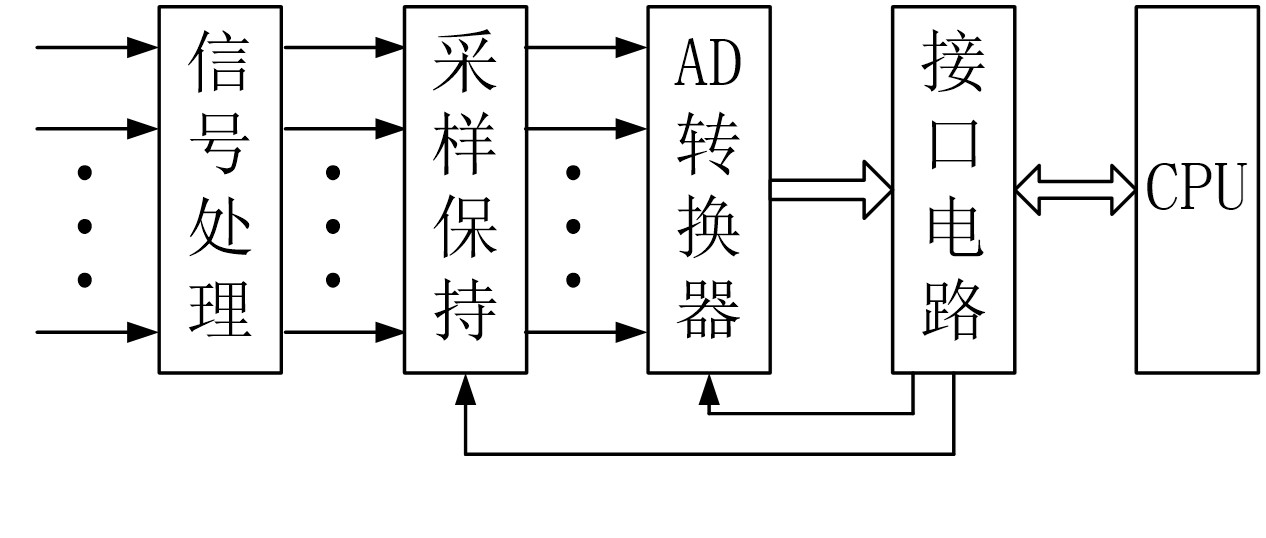
\includegraphics[width=0.4\textwidth]{fig_2_06}\\(a) 并行转换结构\\
  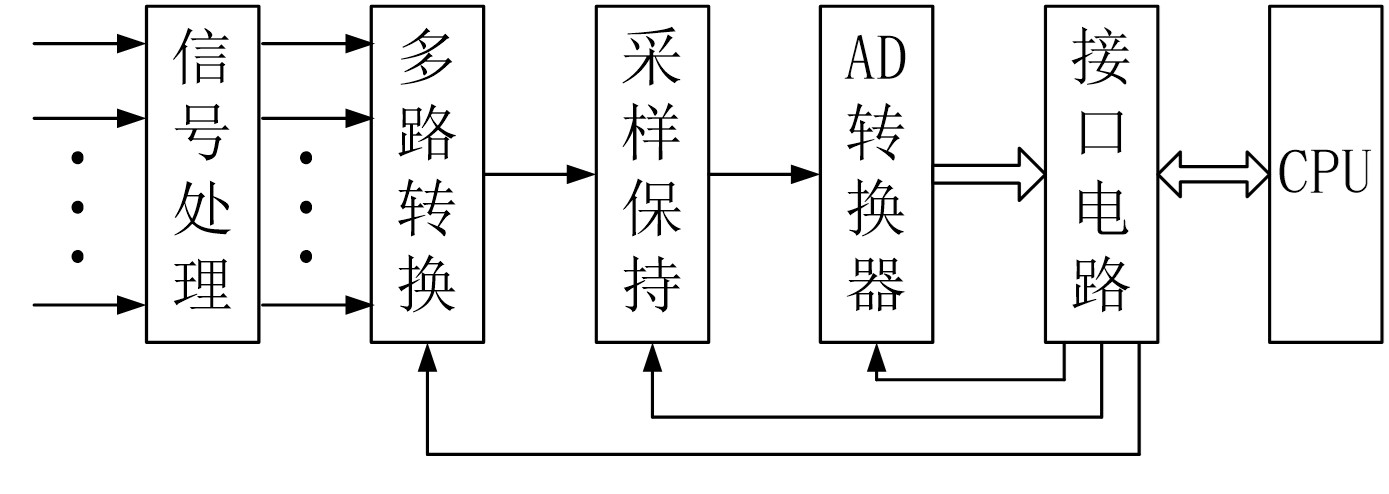
\includegraphics[width=0.4\textwidth]{fig_2_06a}\\(b) 串行(多路通道共享采样保持或模数转换电路)\\
  \caption{模拟量输入通道的结构}\label{fig_2_06}
\end{figure}




\subsection{信号处理}


\begin{itemize}
  \item 信号处理形式
  \begin{itemize}
    \item 信号大小

    \item 电压电流
  \end{itemize}

\begin{figure}[h]
  \centering
  % Requires \usepackage{graphicx}
  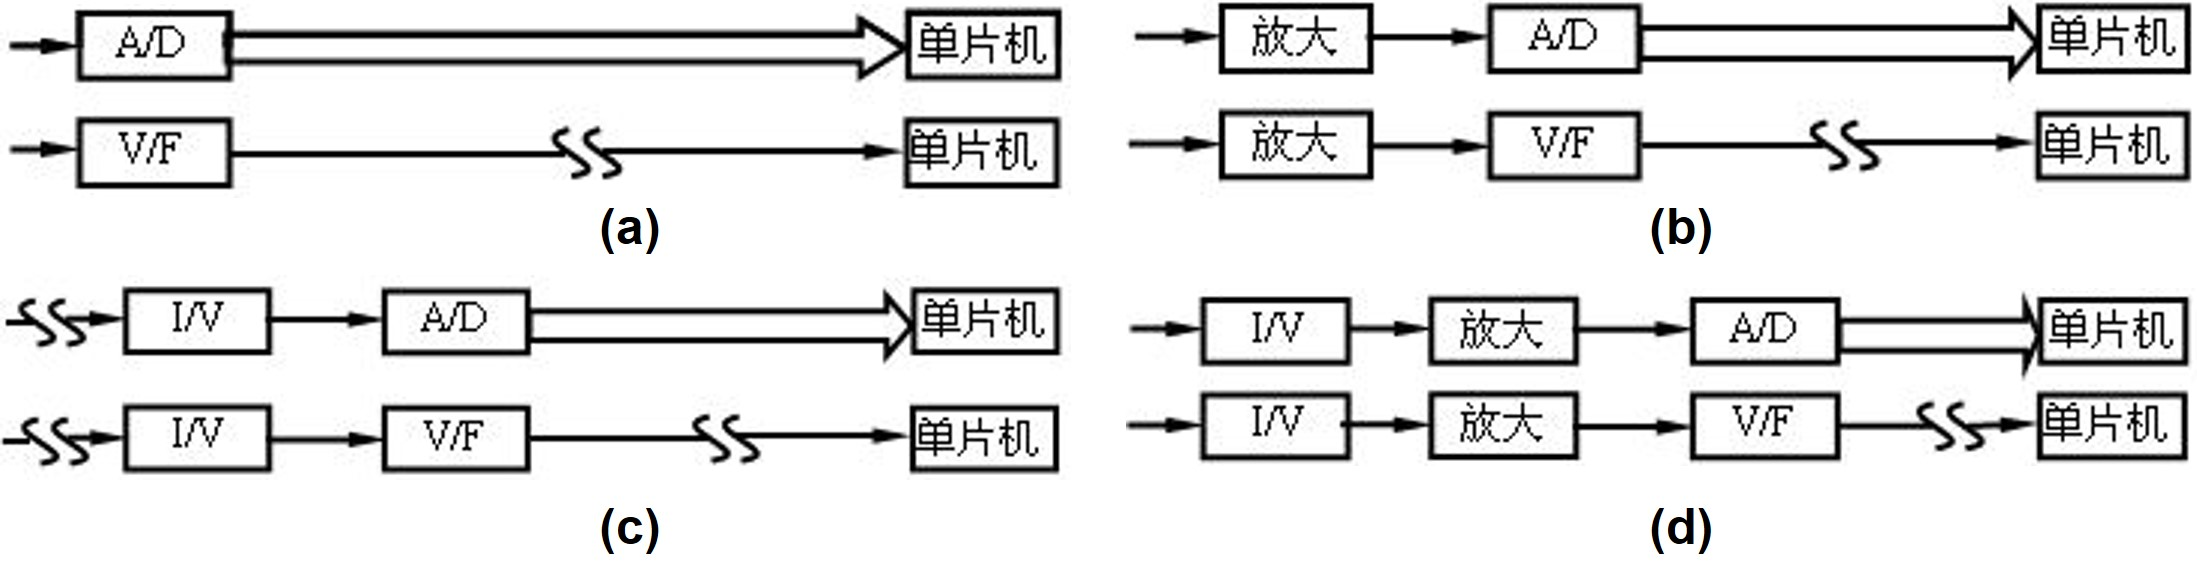
\includegraphics[width=0.8\textwidth]{fig_2_06b}
  \caption{针对不同信号的处理形式,(a)大电压,(b)小电压,(c)大电流,(d)小电流。}\label{fig_2_06b}
\end{figure}


  \item 常用放大电路
  \begin{itemize}
    \item 运算放大器的基本电路
    \item 仪表放大器
    \item 程控放大器
    \item 隔离放大器
  \end{itemize}
  \item I/V变换
  \begin{itemize}
    \item 无源
    \item 有源
  \end{itemize}
\end{itemize}


\subsection{采样保持}

AD转换器将模拟信号转换为数字量需要一定的时间,对于随时间变化的模拟信号来说,转换时间决定了每个采样时刻的最大转换误差。AD 转换延迟所引起的可能误差是$\Delta U$。 对于一定的转换时间,最大可能的误差发生在信号过零的时刻,因为此时dU/dt 最大,转换时间一定,所以$\Delta U$最大,如图\ref{fig_2_07}所示。


\begin{figure}[h]
  \centering
  % Requires \usepackage{graphicx}
  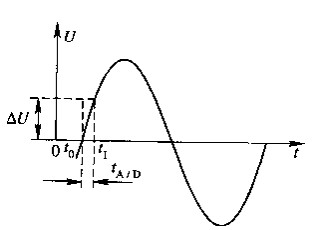
\includegraphics[height=0.15\textheight]{fig_2_07}
  \caption{正弦信号的采样保持}\label{fig_2_07}
\end{figure}


令$U=U_m sin \omega t$,则

\begin{equation}
  dU/dt  =U_m \omega cos \omega t =U_m 2\pi f cos 2\pi ft
\end{equation}

式中,$U_m$为正弦信号的幅值,$f$为信号频率,在坐标原点有:

\begin{equation}
  \Delta U/\Delta t = U_m  2\pi f
\end{equation}

取$\Delta t=t_{A/D}$,则得原点处转换的不确定电压误差为

\begin{equation}
  \Delta U = U_m  2\pi ft_{A/D}
\end{equation}

误差的百分数为:

\begin{equation}
  \sigma =  \Delta U/U_m \times 100\% = 2\pi ft_{A/D}\times 100\%
\end{equation}



实例:一个10位的AD转换器,若要求转换精度为$0.1\%$,转换时间为10μs,则允许转换的正弦波模拟信号的最大频率为

\begin{equation}
  f=\frac{0.1}{2\pi\times10\times10^{-6}\times10^2} \approx 16Hz
\end{equation}

采样/保持器一般由模拟开关、储能元件(电容)、输入和输出缓冲放大器组成。
    采样保持电路有两个工作状态, 一是采样状态.二是保持状态。

选择采样/保持器时,应考虑如下因素:
\begin{enumerate}
  \item 采样保持器的孔径时间:保持命令发出后K完全断开所需时间;

  \item 采样保持器的捕捉时间:由保持到采样时输出U,从原保持值过渡到跟踪信号的时间;

  \item 保持电压变化率:$dU/dt = I_D/C$,其中,$I_D$ 的漏电流。
   \item 常用的采样保持芯片:LF398

\end{enumerate}

应当指出,在模拟量输入通道中,只有在信号变化频率较高而A/D转换速度又不高,以致转换误差影响转换精度时,或者要求同时进行多路采样的情况下,才需要设置采样保持电路,对于一些变化缓慢的生产过程(如石油、化工等)可以不设置保持电路。



\subsection{多路转换器}

多路转换器又称多路开关是用来切换模拟电压信号的关键元件。利用多路开关可将各个输入信号依次地或随机地连接到公用放大器或A/D转换器上 。


\begin{figure}[h]
  \centering
  % Requires \usepackage{graphicx}
  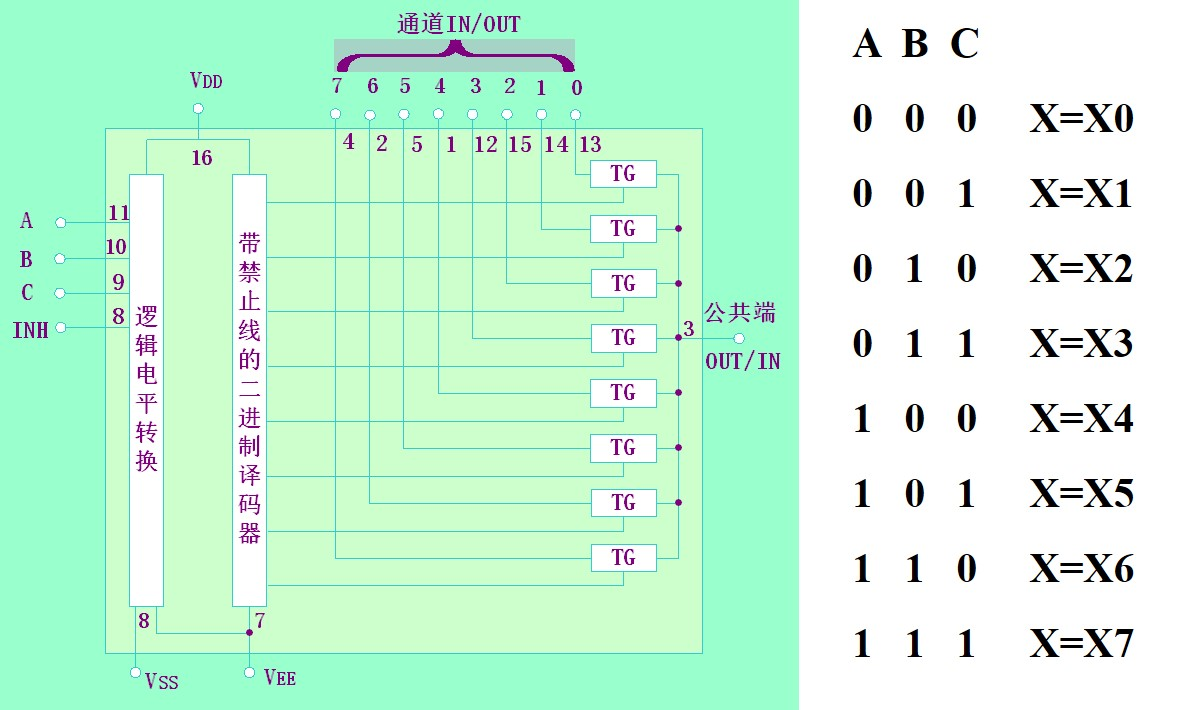
\includegraphics[width=0.6\textwidth]{fig_2_07a}\\
  \caption{多路开关CD4051}\label{fig_2_07a}
\end{figure}


\subsection{A/D转换技术}


\subsubsection{A/D转换原理(1)逐次逼近}

逐次逼近型A/D转换芯片中包括逐次逼近寄存器SAR、D/A转换器、比较器、时序及控制逻辑等部分组成如图\ref{fig_2_08}所示。


\begin{figure}[h]
  \centering
  % Requires \usepackage{graphicx}
  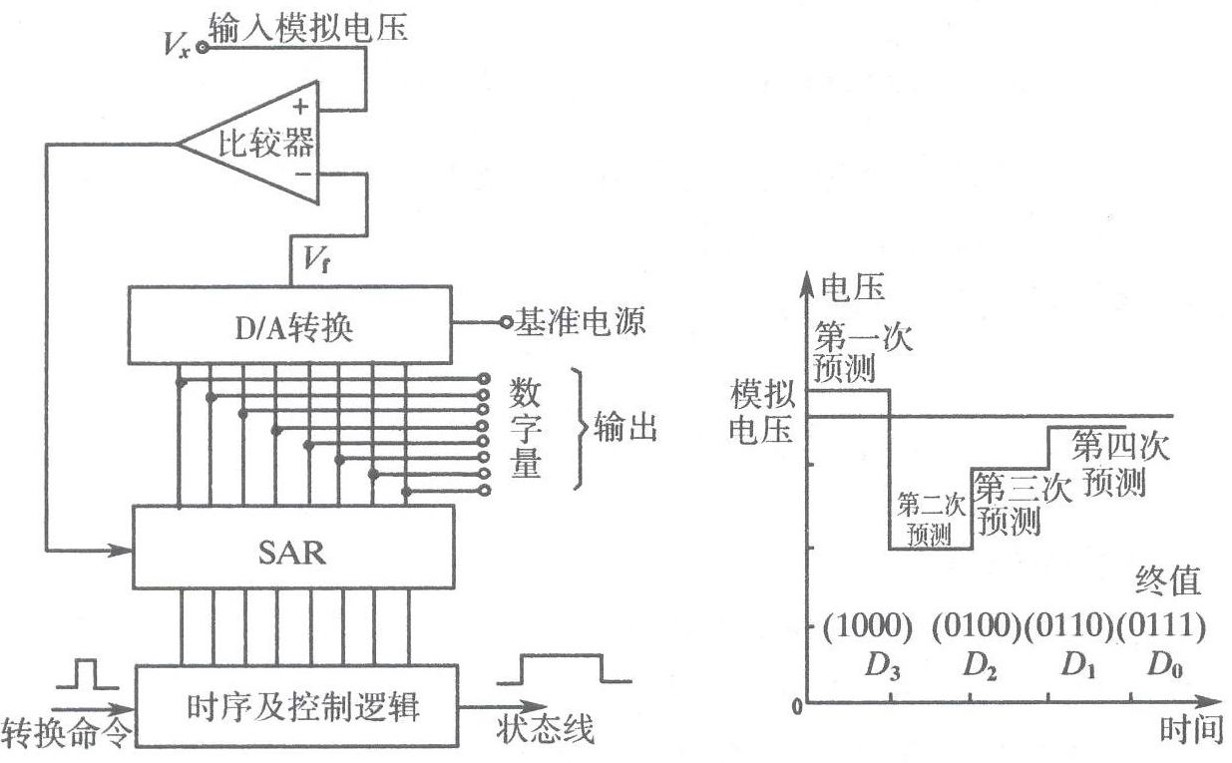
\includegraphics[width=0.6\textwidth]{fig_2_08}\\
  \caption{逐次逼近型A/D}\label{fig_2_08}
\end{figure}

转换过程如下:

\begin{enumerate}
  \item 时序及控制逻辑给SAR最高位为“1”,其余为“0”,经D/A转换为模拟电压Vf ,然后与输入电压Vx 比较,确定该位;
  \item 当Vx ≥Vf ,此位为“1”,置下位为“1”;
  \item 当Vx $<$ Vf ,此位为“0”,置下位为“1”。
  \item 按上述方法依次类推,逐位比较判断,直至确定SAR的最低位为止。
\end{enumerate}




\subsubsection{A/D转换原理(2)双斜率积分}

双斜率积分A/D:器件少、使用方便、抗干扰能力强、数据稳定、价格便宜。典型芯片:MC14433、AD7550、ICL7109\newline

如何理解双斜率积分A/D的工作原理?


首先,明确积分器输出与模拟输入电压之间的关系,如图\ref{fig_2_09} 所示。


\begin{figure}[h]
  \centering
  % Requires \usepackage{graphicx}
  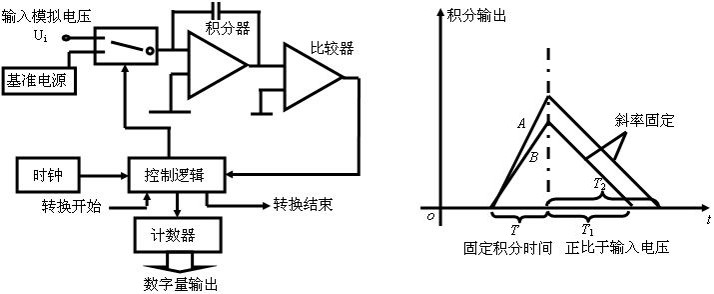
\includegraphics[width=0.6\textwidth]{fig_2_09}\\
  \caption{双斜率积分A/D}\label{fig_2_09}
\end{figure}

  其次,将A/D转换的过程分为两个阶段,即:
  \begin{enumerate}
    \item 模拟开关连接至模拟输入电压。由于模拟输入电压越大,积分器输出电压的变化率就越大。经过固定时间T后,不同大小的输入模拟电压UA、UB 就会达到不同的积分输出。

    \begin{equation}
    -\int_0^T\frac{U_i}{RC}dt=U_o-0
  \end{equation}

  得到


\begin{equation}\label{eq_2_1}
  U_o=-\frac{U_i}{RC}T
  \end{equation}

    \item 模拟开关切换至基准电源(与模拟输入电压极性相反)。由于基础电源的电压值固定,且与原输入电压极性相反,会使积分输出电压以固定斜率(由基准电源电压确定)下降,直至下降到0。 此过程中,利用计数器对这一时间段计时。
              \begin{equation}
    -\int_T^{T+T_1}\frac{U_{REF}}{RC}dt=0-U_o
  \end{equation}
      得到

   \begin{equation}\label{eq_2_2}
  U_o=\frac{U_i}{RC}T_1
  \end{equation}

      由式\ref{eq_2_1}和\ref{eq_2_2}得到:

  \begin{equation}
   -\frac{U_i}{RC}T=\frac{U_i}{RC}T_1
  \end{equation}

  推出:
    \begin{equation}
   {U_i}=-\frac{T_1}{T}U_{REF}
  \end{equation}

  即$U_i\propto T_1$



  \end{enumerate}

  易知:模拟输入电压与积分输出电压下降至0的时间为正比关系。因而,可用计数器的数字量输出表示输入电压的大小。







\subsubsection{A/D转换原理(3)$\Sigma-\Delta$型}

工作原理:模拟信号与1位DAC的输出送到减法器,经积分器后送到比较器。以Kfs采样速率将输入信号转换为由1和0构成的连续串行位流。精度最高的A/D转换器,一般说来速度较低。典型芯片:AD7715

\begin{figure}[h]
  \centering
  % Requires \usepackage{graphicx}
  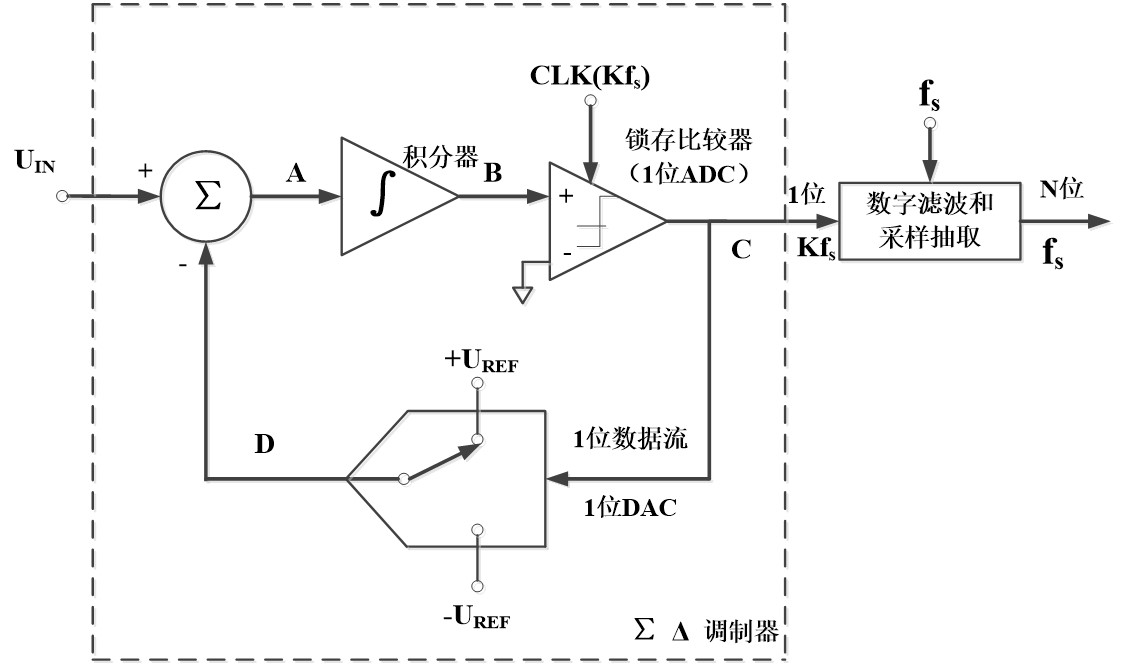
\includegraphics[width=0.6\textwidth]{fig_2_10}\\
  \caption{$\Sigma-\Delta$型A/D}\label{fig_2_10}
\end{figure}


\begin{figure}[h]
  \centering
  % Requires \usepackage{graphicx}
  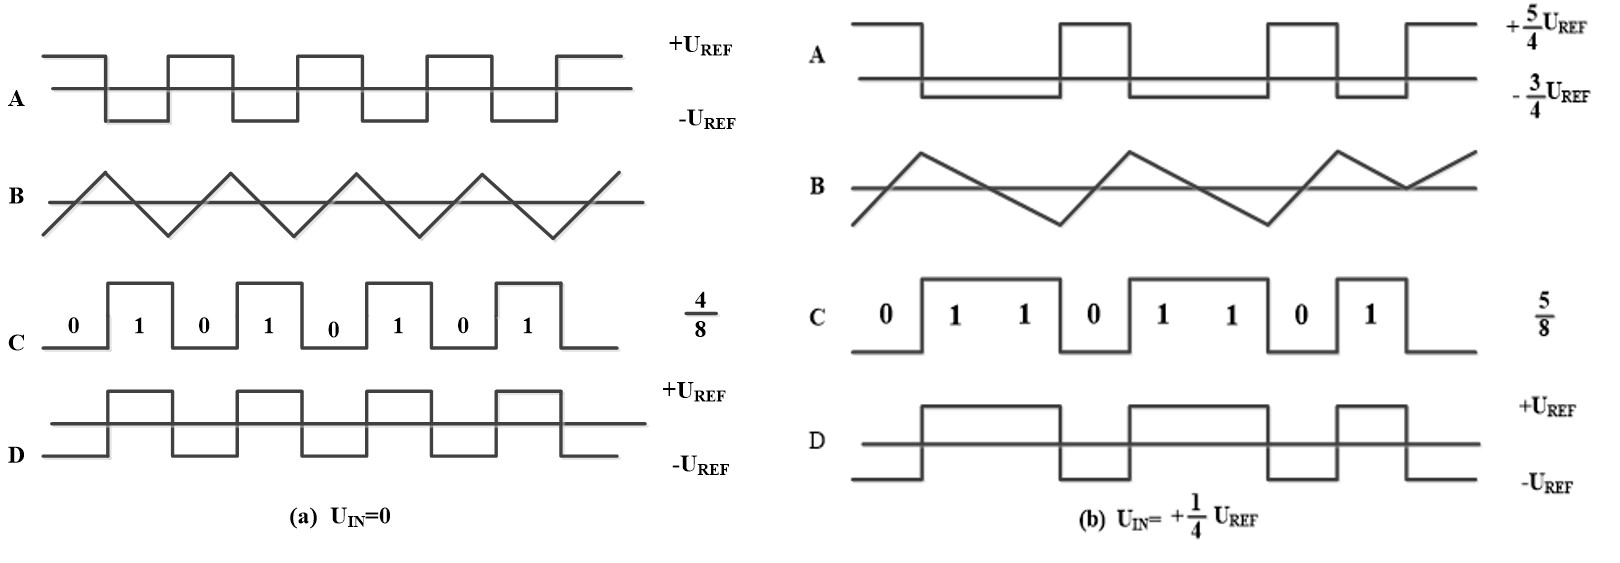
\includegraphics[width=0.9\textwidth]{fig_2_10a}\\
  \caption{$\Sigma-\Delta$型A/D举例}\label{fig_2_10a}
\end{figure}

\begin{remark}ADI公司提供的演示视频:

  http://designtools.analog.com/dt/sdtutorial/sdtutorial.html
\end{remark}


\subsubsection{A/D技术指标}



\begin{itemize}
  \item 分 辨 率

  分辨率通常用数字输出最低有效位(Least Significant Bit,LSB)所对应的模拟量输入电压值表示,例如:AD 位数n=8,满量程为5V,则LSB对应$5V/(2^8-1)=19.6mV$。
     由于分辨率直接与转换位数有关,所以一般也用其位数表示分辨率,如8,10、12、14、16为AD。
     通常把小于8位的称为低分辨率,10-12位的成为中分辨率,14位以上的为高分辨率。

  \item 转换时间

  从发出转换命令信号到转换结束信号有效的时间间隔,即完成一次转换所用的时间,为转换时间。转换时间的倒数为转换速率。
      通常转换时间从几ms到100ms成为低速,从几μs到100μs称为中速,从10ns到100ns左右成为高速。

  \item 转换量程

         所能转换的模拟量输入电压范围,如0-5V,-5 -+5V 等。

\end{itemize}



\subsubsection{A/D实现技术}

A/D转换器与CPU连接时需要考虑的问题

\begin{itemize}
  \item 输入模拟电压的连接
  \begin{itemize}
    \item 单端输入:IN直接与信号连接
    \item 差动输入:VIN(+) VIN(-)
    \begin{itemize}
      \item 单端输入正信号:UIN(+)接信号、UIN(-)接地
      \item 单端输入负信号: UIN(-)接信号、UIN(+)接地。

    \end{itemize}



  \end{itemize}




  \item 数据输出线和系统总线的连接
  \begin{itemize}
    \item 数据线具有可控三态输出门,可直接与系统总线连接;

    \item 数据线没有三态输出门或具有内部三态门但不受外部控制,则(不能直接连接系统总线)必须通过I/O接口连接;

    \item 8位以上A/D转换需考虑A/D的数据输出线和系统总线位数的对应关系(针对8位CPU、 12位A/D,需分高低位分别连接,分时按字节读入)。

        \begin{itemize}
    \item A/D位数=数据总线位数
    \item 	A/D位数$>$数据总线位数

    \item A/D位数$<$数据总线位数

  \end{itemize}
\end{itemize}




\end{itemize}






\section{模拟量输出通道}


\subsection{模拟量输出通道的结构}


一个实际的计算机控制系统中,往往需要多路的模拟量输出,其实现方法有两种:

\begin{enumerate}
  \item 数字保持式结构:一个通路一个D/A转换器,CPU 与D/A 之间通过独立的接口缓冲器传送信息。

      特点:速度快,精度高,可靠,互不影响;D/A多。

  \item 模拟保持式结构:多个通路共用一个D/A,CPU分时将各路D/A转换通过多路开关分送各路保持电路去。

特点:省D/A,速度慢,可靠性较差。

\end{enumerate}

\begin{figure}[h]
  \centering
  % Requires \usepackage{graphicx}
  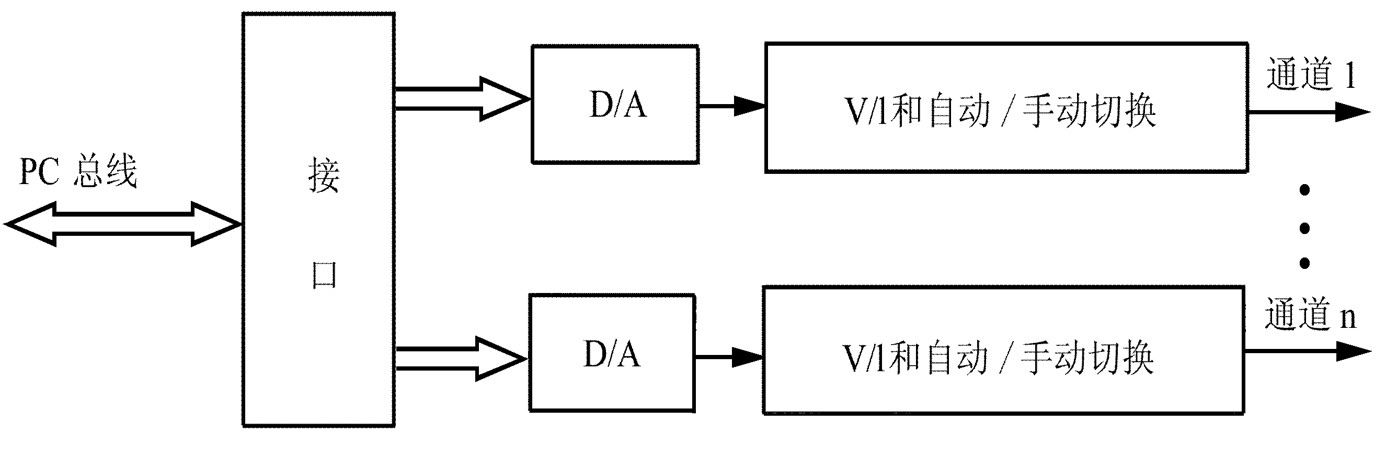
\includegraphics[width=0.6\textwidth]{fig_2_11}\\(a) 数字保持式\\
  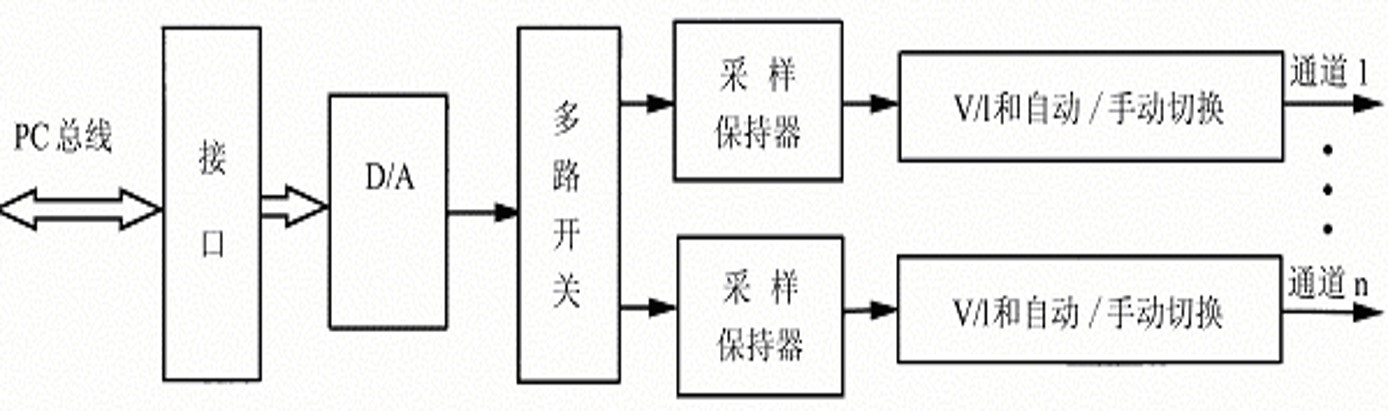
\includegraphics[width=0.6\textwidth]{fig_2_11a}\\(b) 模拟保持式
  \caption{模拟量输出通道的结构}\label{fig_2_11}
\end{figure}

\subsection{D/A转换技术}






\subsubsection{D/A转换原理(1)分类}

依据D/A转换原理不同可分为:

\begin{itemize}
\item 求取脉冲平均值的PWM型

\item 数字编码信号控制下加权量叠加型
\end{itemize}

加权量叠加型一般由四部分组成,即电子开关、电阻网络、放大器和标准电压源;根据电阻网络不同,可分为权电阻译码D/A转换器、倒T 型网络D/A转换器等,如图\ref{fig_2_12}、\ref{fig_2_12a}所示。



\subsubsection{D/A转换原理(2)权电阻D/A转换器}





图\ref{fig_2_12}所示权电阻D/A转换器,运算放大器的输入电流为:





\begin{equation}
  I = \sum_{i=0}^{n-1}I_i = \sum_{i=0}^{n-1} \frac{U_R}{2^{n-1}R}D_i2^i = \frac{U_R}{2^{n-1}R}\sum_{i=0}^{n-1} D_i2^i
\end{equation}


运算放大器的输出电压为:


\begin{equation}
  U=-IR_f  =-\frac{U_RR_f}{2^{n-1}R}\sum_{i=0}^{n-1} D_i2^i
\end{equation}

若$R_f = 1/2R$,代入上式得

\begin{equation}
  U=- \frac{U_RR_f}{2^{n-1}R}\sum_{i=0}^{n-1} D_i2^i = -\frac{U_R}{2^{n-1}}\sum_{i=0}^{n-1} D_i2^i
\end{equation}


当D/A的输入数据为0时,

\begin{equation}
  U=0
\end{equation}

当D/A的输入数据为$0x1...11H$时,

\begin{equation}
  U_m=-\frac{2^n-1}{2^n}U_R
\end{equation}

因而U的变化范围是

\begin{equation}
  0-\frac{2^n-1}{2^n}U_R
\end{equation}

\begin{figure}
  \centering
  % Requires \usepackage{graphicx}
  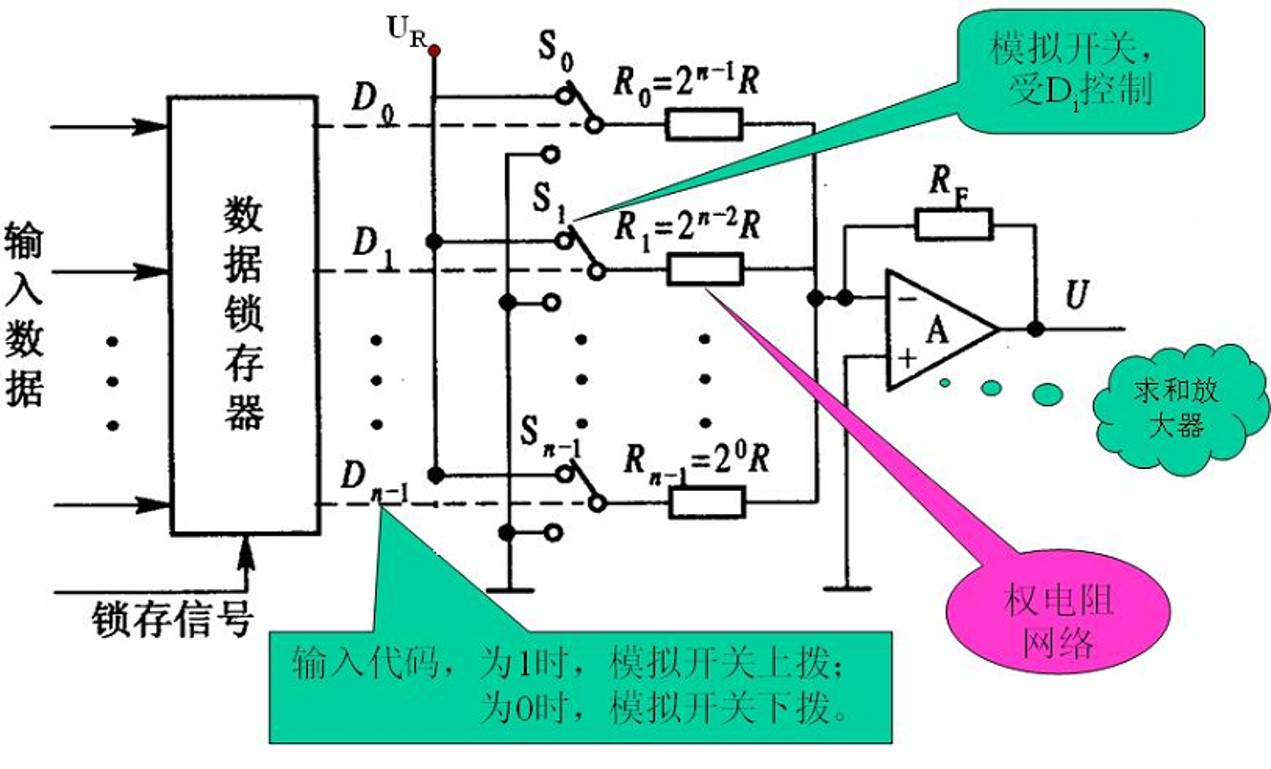
\includegraphics[width=0.5\textwidth]{fig_2_12}
  \caption{权电阻D/A}\label{fig_2_12}
\end{figure}


\subsubsection{D/A转换原理(3)倒T型网络D/A转换器}

如图\ref{fig_2_12a} 所示,Di=1,Si将电阻接到运放反向输入端;Di=0, Si将i将电阻接到运放同向输入端;都是虚地,各支路电流不会变化;流入2R支路的电流是以2的倍速递减;

\begin{eqnarray}
  I_\Sigma &=& D_{n-1}\frac{I}{2^1} +D_{n-2}\frac{I}{2^2}+...+D_{1}\frac{I}{2^{n-1}}+D_{0}\frac{I}{2^{n}}\\
&=&\frac{I}{2^{n}} (D_{n-1}2^{n-1} + D_{n-2}2^{n-2} + ... + D_{1}2^{1} + D_{0}2^{0})\\
&=&\frac{I}{2^{n}}\sum_{i=0}^{n-1} D_i2^i
\end{eqnarray}


运算放大器的输出电压为:

\begin{equation}
  U=-I_\Sigma R_f  =- \frac{IR_f}{2^{n}}\sum_{i=0}^{n-1} D_i2^i
\end{equation}

若$R_f=R$,并将$I=U_R/R$代入上式,则有
\begin{equation}
  U=-I_\Sigma R_f  =- \frac{U_R}{2^{n}}\sum_{i=0}^{n-1} D_i2^i
\end{equation}

可知,输出模拟电压正比于数字量的输入。



\begin{figure}
  \centering
  % Requires \usepackage{graphicx}
  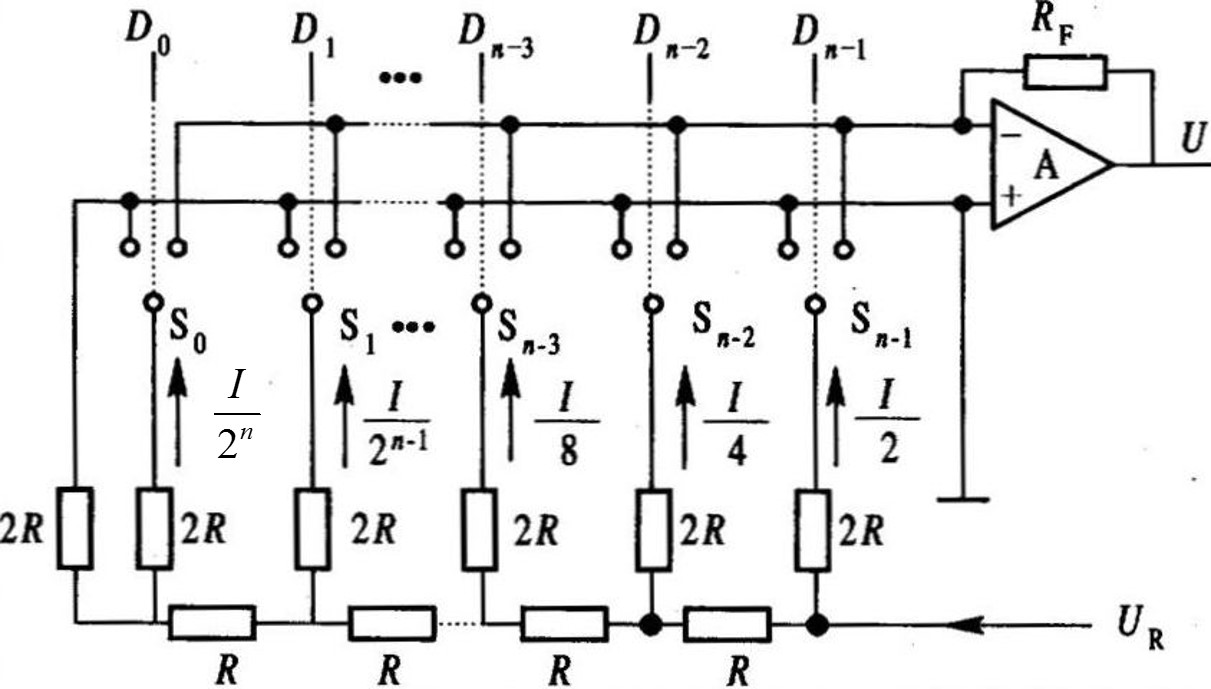
\includegraphics[width=0.5\textwidth]{fig_2_12a}
  \caption{倒T型网络D/A转换器}\label{fig_2_12a}
\end{figure}


\subsubsection{D/A技术指标}


\begin{description}
  \item[分 辨 率] 与A/D转换器的分辨率概念类似,指当输入数字量变化1时,输出模拟量变化的大小。分辨率通常用数字量的位数来表示,如8 位、12位、18 位。
  \item[稳定时间] 指D/A转换器所有输入二进制数变化是满刻度时,模拟量输出稳定到±1/2LSB范围内所需要的时间。一般为几十纳秒到几微秒完程一次转换所需要的时间;

  \item[线 性 度] 一个理想的D/A转换器输入输出特性应是线性的。在满量程范围内,偏离理想转换特性的最大误差称为线性误差,一般用LSB的分数表示。
\end{description}




\subsubsection{D/A实现技术}


如图\ref{fig_2_13}所示为DAC0832的原理图。
在使用DAC0832时应注意以下两个内容:

\begin{figure}
  \centering
  % Requires \usepackage{graphicx}
  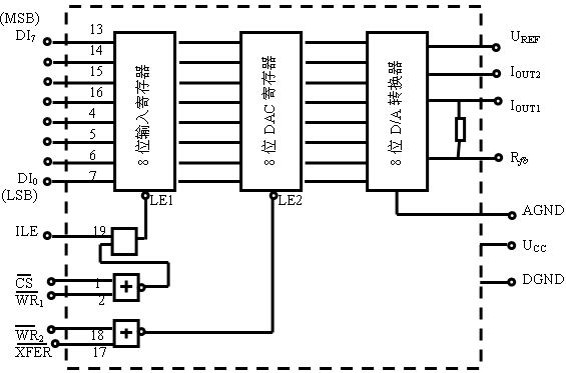
\includegraphics[width=0.5\textwidth]{fig_2_13}
  \caption{DAC0832}\label{fig_2_13}
\end{figure}


\begin{itemize}
  \item 极性:如图\ref{fig_2_14}所示;
  \item 与CPU接口--缓冲方式:如图\ref{fig_2_15}所示。
\end{itemize}

\begin{figure}
  \centering
  % Requires \usepackage{graphicx}
  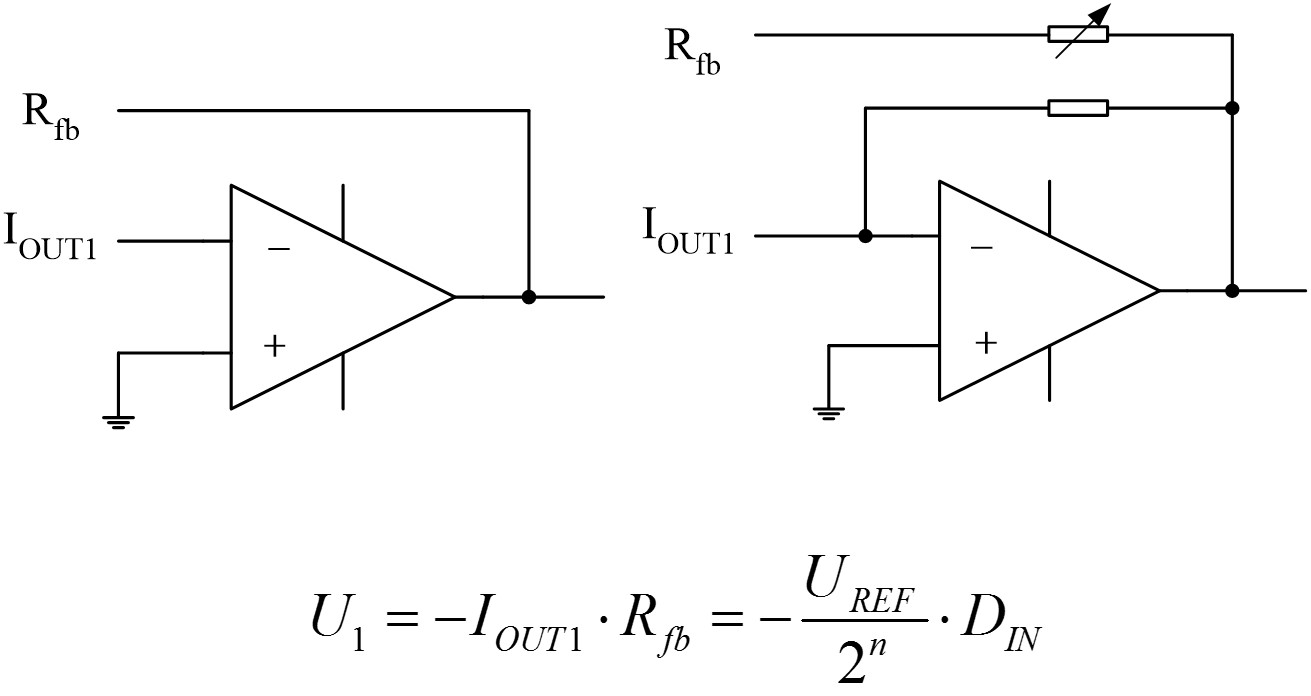
\includegraphics[width=0.45\textwidth]{fig_2_14}(a)
  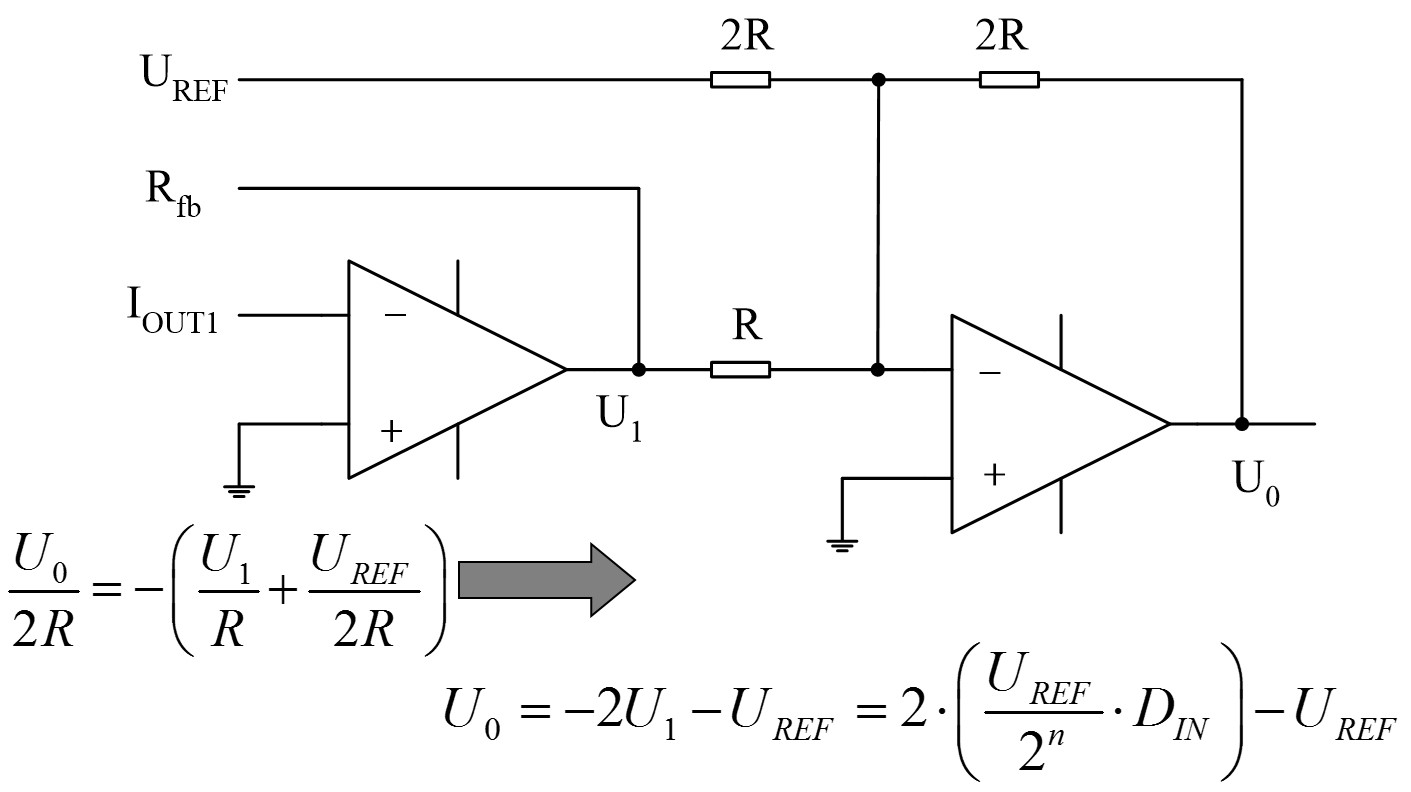
\includegraphics[width=0.45\textwidth]{fig_2_14a}(b)
  \caption{模拟输出极性变换}\label{fig_2_14}
\end{figure}


\begin{figure}
  \centering
  % Requires \usepackage{graphicx}
  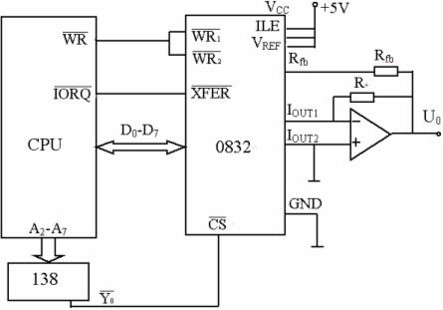
\includegraphics[width=0.45\textwidth]{fig_2_15}(a)
  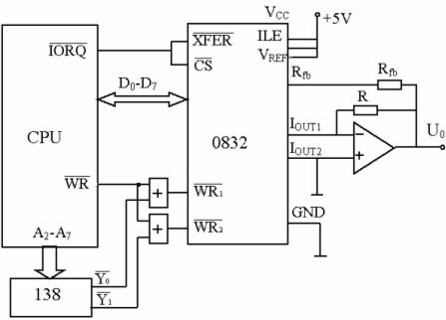
\includegraphics[width=0.45\textwidth]{fig_2_15a}(b)
  \caption{与CPU的接口---缓冲方式}\label{fig_2_15}
\end{figure}






\section{本章要点总结}

\begin{itemize}

\item 过程通道的概念及组成;
\item 编址方式的种类和特点;
\item 常用的地址译码方法,重点理解译码器译码的设计方法;
\item 总线接口常用芯片的使用;
\item 数字量输入通道的结构,并了解其信号调理方式;
\item 数字量输出通道的结构,并了解其输出调理电路设计;
\item 模拟量输入通道的结构,常见到信号处理形式;
\item 了解信号放大,I/V变换的种类以及原理;
\item 理解采样保持的使用以及采样/保持器的概念和作用;
\item 逐次逼近式和双积分式A/D转换的原理;
\item A/D转换器的技术指标;
\item A/D转换器与计算机的接口方法;
\item 模拟量输出通道的一般结构和特点;
\item 权电阻和倒T型网络D/A转换器原理;
\item D/A转换器的技术指标;
\item DAC0832与CPU的接口方法及输出极性的变换;


\end{itemize}

\setcounter{chapter}{2}

\chapter{测量数据处理}

\section{信号的采样和量化}

\subsection{采样过程}

典型的计算机控制系统的结构,如图\ref{fig_3_01}所示。连续信号$f(t)$通过采样开关后,转变为脉冲序列$f^*(t)$的过程,如图\ref{fig_3_02}所示。


\begin{figure}[h]
  \centering
  % Requires \usepackage{graphicx}
  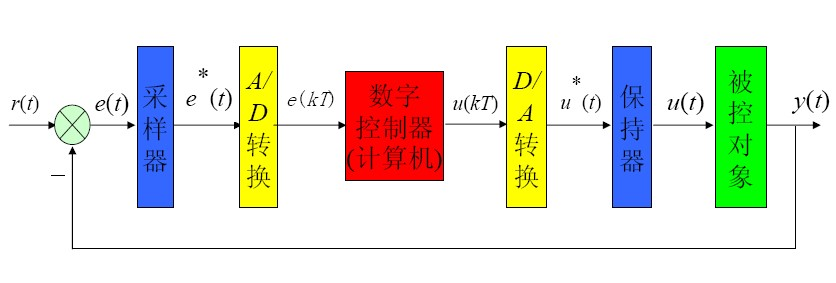
\includegraphics[width=0.6\textwidth]{fig_3_01}\\
  \caption{典型的计算机控制系统的结构}\label{fig_3_01}
\end{figure}


\begin{figure}[h]
  \centering
  % Requires \usepackage{graphicx}
  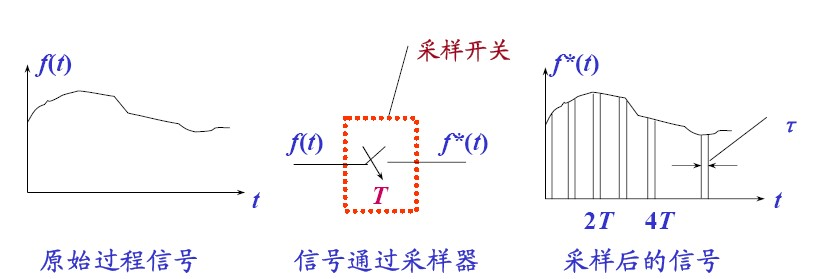
\includegraphics[width=0.6\textwidth]{fig_3_02}\\
  \caption{过程连续信号采样过程示意图}\label{fig_3_02}
\end{figure}

时域描述:

\begin{eqnarray}
% \nonumber to remove numbering (before each equation)
  f_s &=& \frac{1}{T} \\
  \omega_s &=& \frac{2\pi}{T}=2\pi f_s
\end{eqnarray}

其中,采样周期T(s),
闭合时间$\tau$(s),
采样角频率$\omega_s$(rad/s),
采样频率$f_s$(Hz)。



理想的单位脉冲函数为:

\begin{displaymath}
\left\{ \begin{array}{ll}
\delta(t)=\infty, & \textrm{for $t=0$}\\
\delta(t)=0 & \textrm{for $t\neq 0$}\\
\int_{-\infty}^{+\infty} \delta(t)dt=1 &
\end{array} \right.
\end{displaymath}

设$\delta (t-kT)$ 是$t=kT$时刻的理想采样脉冲,则

\begin{equation}
  f^*(t)=f(t)\sum_{k=0}^\infty\delta(t-kT)
\end{equation}


因为$f^*(t)$只与$f(t)$在脉冲出现瞬间的值 $f(kT)$有关,故采样信号可用下式表示:

\begin{equation}
  f^*(t)=f(t)\sum_{k=0}^\infty f(kT)\delta(t-kT) = f(t)\delta_T(t)
\end{equation}



\subsection{采样定理}


对于连续信号$f(t)$,记其傅立叶变换为$F(j\omega)$。则对于离散后的采样信号$f^*(t)$,其傅立叶变换后,为:

\begin{equation}
  F^*(j\omega)=\frac{1}{T}\sum_{k=-\infty}^{+\infty}F(j\omega-jk\omega_s)
\end{equation}

由上式可知,$F^*(j\omega)$由$F(j\omega)$向两端无限延拓而成,且幅值上相差$\frac{1}{T}$。此时,$\omega_s$与$\omega_{max}$的大小关系就对$F^*(j\omega)$的形态产生影响,如图\ref{fig_3_03}所示。


\begin{figure}[h]
  \centering
  % Requires \usepackage{graphicx}
  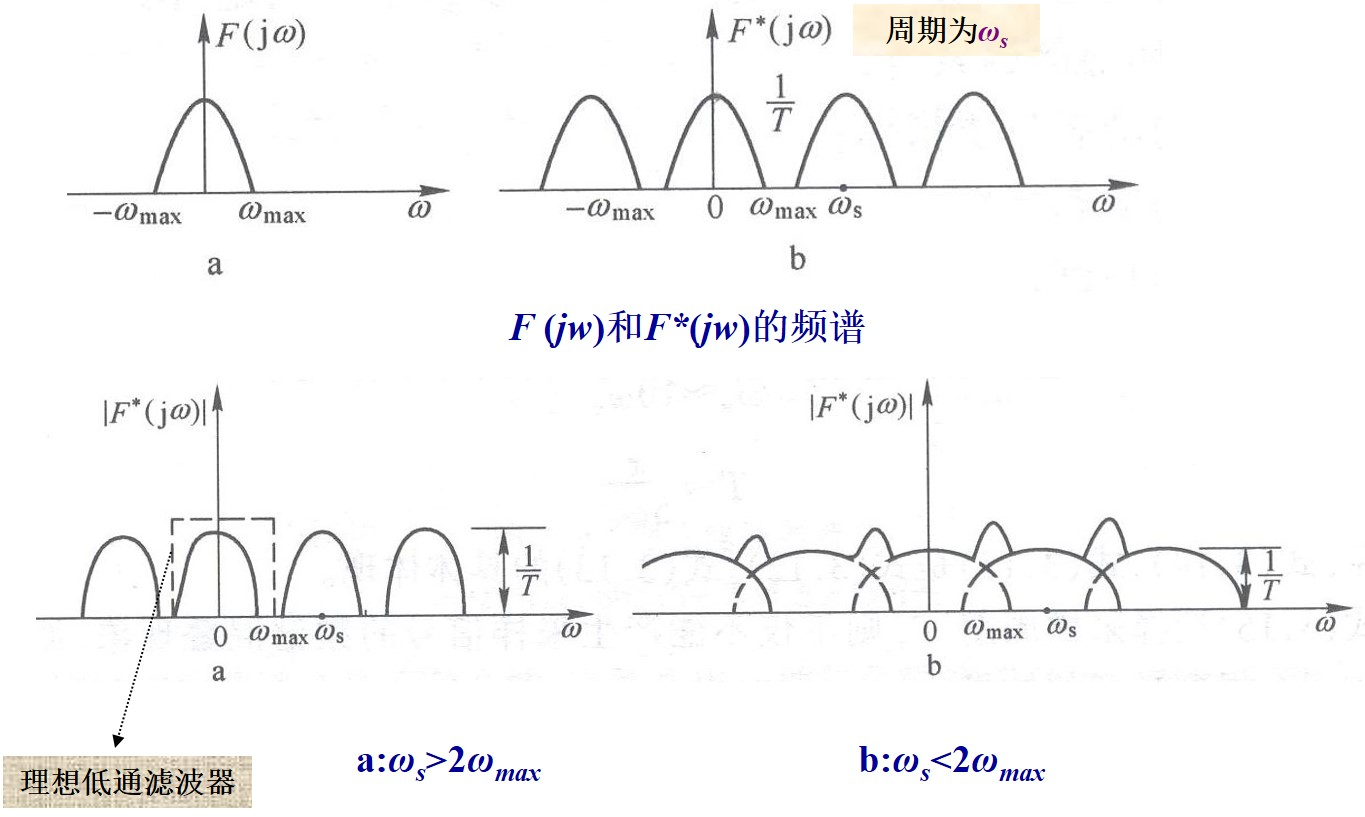
\includegraphics[width=0.6\textwidth]{fig_3_03}\\
  \caption{采样信号频谱的两种情况}\label{fig_3_03}
\end{figure}






\begin{remark}

 \textbf{香农采样定理}:一个连续时间信号$f(t)$,设其频带宽度是有限的,其最高频率为$\omega_{max}$(或$f_{max}$)。如果在等间隔点上对该信号$f(t)$ 进行连续采样,为了使采样后的离散信号$f^*(t)$ 能包含原信号$f(t)$的全部信息量,则采样角频率必须满足以下关系:

$\omega_{s}\ge2\omega_{max}$ 或者 $T_s\le \frac{T_{max}}{2}$

采样后的离散信号$f^*(t)$才能无失真地复现$f(t)$。

其中,$\omega_s=2\pi f_s=\frac{2\pi}{T_s}$

\end{remark}





\subsection{采样频率的选择}

常见过程参数的采样周期T,如图\ref{fig_3_04}所示。

\begin{figure}[h]
  \centering
  % Requires \usepackage{graphicx}
  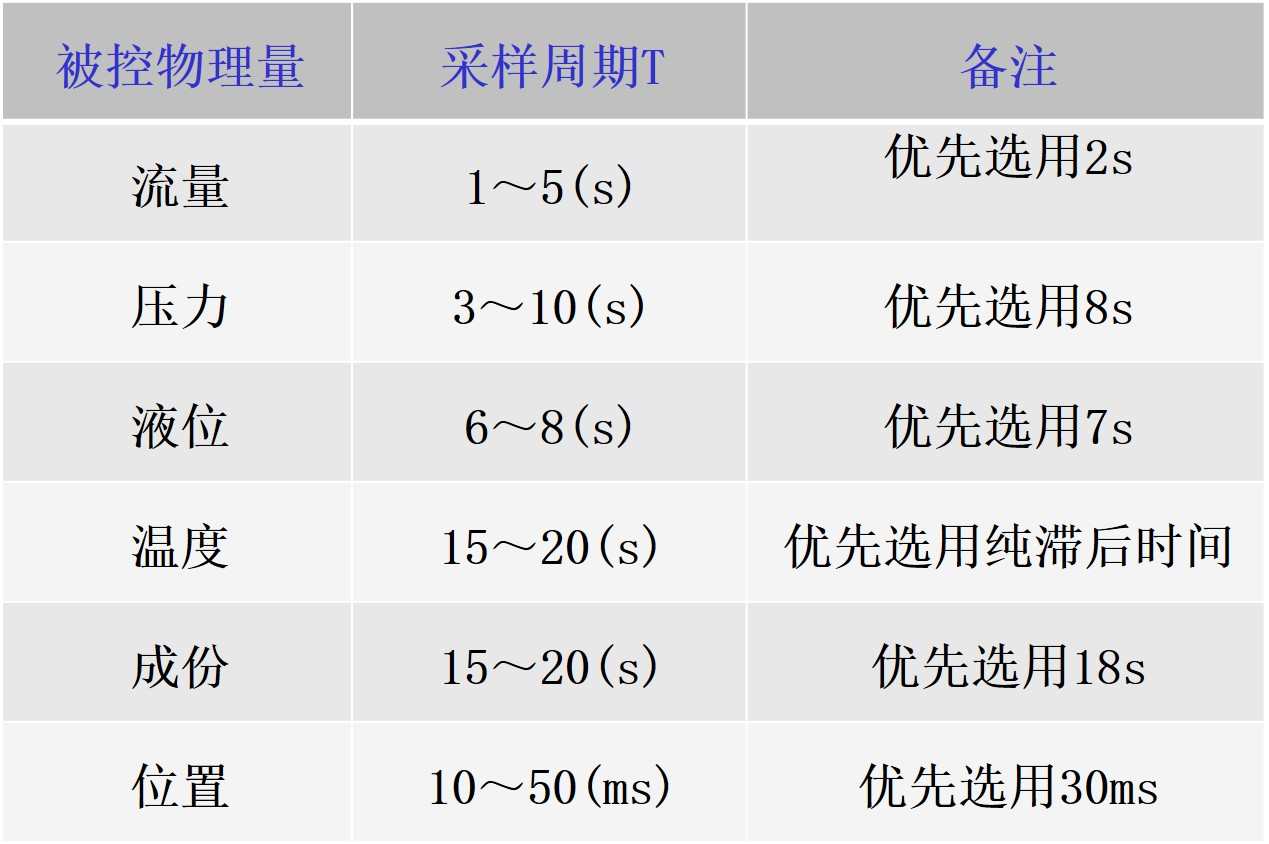
\includegraphics[width=0.4\textwidth]{fig_3_04}\\
  \caption{采样周期的选取}\label{fig_3_04}
\end{figure}





\section{线性化处理}


计算机从工程输入通道得到的现场信号与该信号所代表的对应的物理量之间不一定是线性关系,经常存在着非线性关系。
例如,在温度测量中,常用的Pt100铂电阻,其适用范围为(-200℃,850℃)。根据IEC 标准751-1983规定,Pt100铂电阻的阻值与温度的关系为


\begin{displaymath}
\left\{ \begin{array}{ll}
R_t = R_0[1+At+Bt^2+C(t-100)t^3], & \textrm{$-200\le t \le 0$}\\
R_t = R_0[1+At+Bt^2], & \textrm{$0 < t \le 850$}
\end{array} \right.
\end{displaymath}

再如在流量测量中,孔板测量气体或液体的流量,差压变送器输出的孔板差压信号ΔP,同实际流量F之间成平方根关系,即:

\begin{equation}
  F=K\sqrt{\Delta P}
\end{equation}
式中,K 是流量系数,也是非线性关系。

非线性补偿的三种方法:

\begin{enumerate}
  \item 公式计算法:适用于解析式明确的非线性函数关系;
  \item 查表法;
  \item 线性插值法,即:
  \begin{equation}
y=y_i+\frac{y_{i+1}-y_i}{x_{i+1}-x_i}(x-x_i)
\end{equation}
\end{enumerate}




\section{标度变换}

\textbf{标度变换}:测量值(进入计算机的二进制)与工程值的转换(实际温度、压力、流量)。\textbf{目的}:为了进行显示、记录、打印以及报警,必须将数字量转换成不同量纲,以便操作人员进行监视和管理生产。






\subsection{线性参数标度变换}

一般可采用以下公式进行变换:

\begin{equation}
A_x=\frac{N_{X}-N_0}{N_{M}-N_0}(A_M-A_0)+A_0
\end{equation}

例:某热处理炉温度测量表的量程为200到800摄氏度。在某一时刻,计算机采样并经数字滤波后的数字量为CDH,求此时对应的温度。

解:略。

\subsection{非线性参数标度变换}

(一)如被测量为非线性刻度时,其标度变换应具体分析,如:流量测量中,其流量与差压的公式为:
\begin{equation}
  F=K\sqrt{\Delta P}
\end{equation}

      测量流量时的标度变换公式为:
\begin{equation}
\frac{G_X-G_0}{G_M-G_0}=\frac{K\sqrt{\Delta N_X}-K\sqrt{\Delta N_0}}{K\sqrt{\Delta N_M}-K\sqrt{\Delta N_0}}
\end{equation}

(二)线性化处理

级数展开法:该方法的思想是利用泰勒级数展开把一些计算机基本指令集不包含的数学运算转换为更为便捷的乘加运算。例如,$y=\sqrt{x}$在$x=1$附近的级数展开为:

\begin{equation}
y=\sqrt{x}=1+\frac{1}{2}(x-1)-\frac{1}{8}(x-1)^2+\frac{1}{16}(x-1)^3+\ldots
\end{equation}

线性化处理还可通过迭代法实现,常用的有牛顿迭代法。迭代公式依据原计算公式而确定。上式所对应的牛顿迭代公式为:

\begin{equation}
y_{k+1}=\frac{1}{2}(y_{k}+\frac{x}{y_{k}})
\end{equation}



\section{越限报警处理}

超限报警分为上限报警、下限报警及上下限报警。

\begin{enumerate}
  \item 上限报警��

       若Xn>Xmax,则上限报警,否则继续执行原定操作。
  \item 下限报警��

      若Xn<Xmin,则下限报警,否则继续执行原定操作。��
  \item 上下限报警��

      若Xn>Xmax,则上限报警,否则对下式作判别:Xn<Xmin?若是,则下限报警,否则继续原定操作。
\end{enumerate}

图\ref{fig_3_05}为简单的上下限报警流程图。图\ref{fig_3_06}为考虑越限次数的报警流程图。
\begin{figure}[h]
  \centering
  % Requires \usepackage{graphicx}
  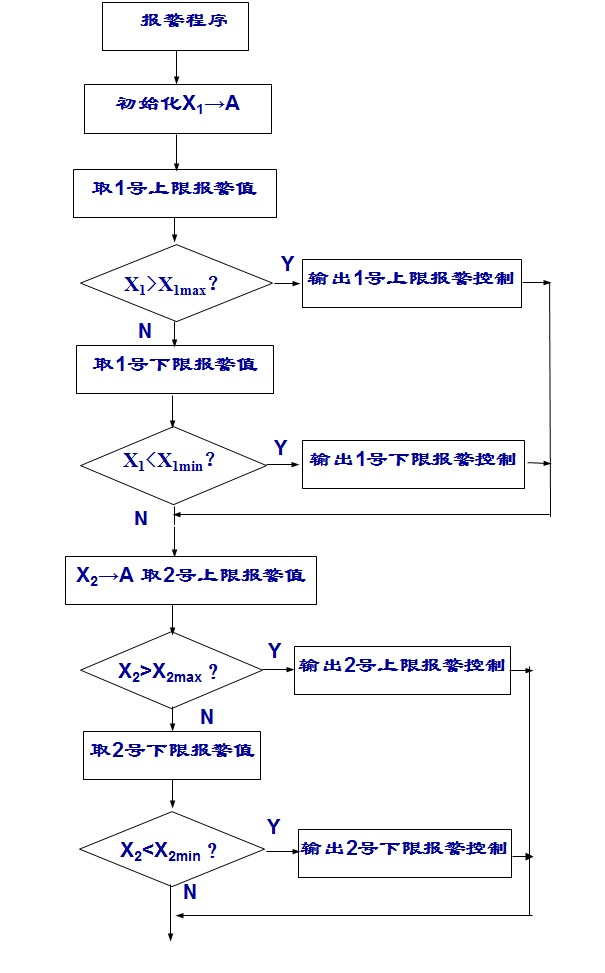
\includegraphics[width=0.4\textwidth]{fig_3_05}\\
  \caption{简单的上下限报警流程图}\label{fig_3_05}
\end{figure}

\begin{figure}[h]
  \centering
  % Requires \usepackage{graphicx}
  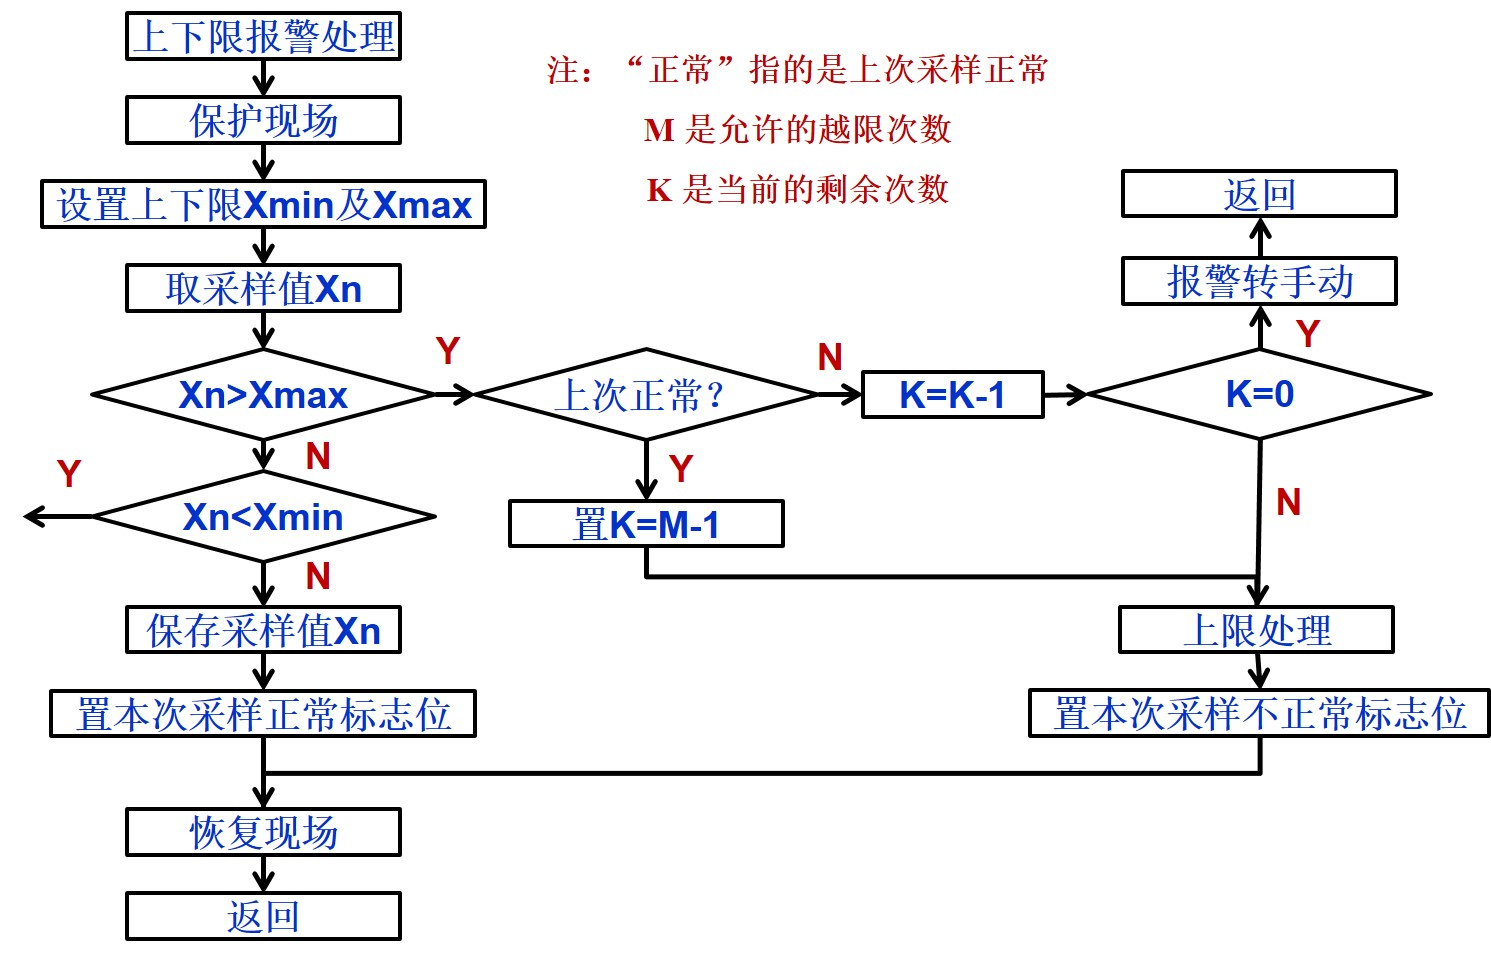
\includegraphics[width=0.7\textwidth]{fig_3_06}\\
  \caption{考虑越限次数的报警流程图}\label{fig_3_06}
\end{figure}




\section{数字滤波技术}

实质上它是一种程序滤波。  数字滤波克服了模拟滤波器的不足,它与模拟滤波器相比,有以下几个优点:
\begin{itemize}
  \item 数字滤波是用程序实现的,可多个通道公用一个滤波程序;

  \item 不需要增加硬设备,所以可靠性高,稳定性好,不存在各个回路之间的阻抗匹配问题;

  \item 数字滤波可以对很低的频率进行滤波;

  \item 数字滤波器可根据信号的不同,采用不同的滤波方法或滤波参数,具有灵活、方便、功能强的特点。

\end{itemize}


\subsection{程序判断滤波方法}

(1)限幅滤波—消除幅度较大的尖峰干扰

如果$|Y_n-Y_{n-1}|\le \Delta y$,则取$Y_n$; 如果$|Y_n-Y_{n-1}|> \Delta y$,则取$Y_{n-1}$。

(2)限速滤波—消除高频干扰

如果$|Y_2-Y_{1}|\le \Delta y$,则取$Y_2$; 如果$|Y_2-Y_{1}|> \Delta y$,则存$y_2$,采$Y_{3}$;
如果$|Y_3-Y_{2}|\le \Delta y$,则取$Y_3$; 如果$|Y_3-Y_{2}|> \Delta y$,则取$({Y_{2}+Y_{3}})/2$;


\begin{remark}
程序判断滤波法

  A、方法:根据经验判断,确定两次采样允许的最大偏差值(设为A),每次检测到新值时判断:如果本次值与上次值之差<=A,则本次值有效。如果本次值与上次值之差>A,则本次值无效,放弃本次值,用上次值代替本次值

  B、优点:能有效克服因偶然因素引起的脉冲干扰。

  C、缺点:无法抑制那种周期性的干扰,平滑度差。
\end{remark}

\subsection{中值滤波方法}

这种滤波法是将被测参数连续采样N次(一般N取奇数),然后把采样值按大小顺序排列,再取中间值作为本次的采样值。消除脉冲性质的干扰。
\begin{remark}
  中位值滤波法

A、方法:连续采样N次(N取奇数),把N次采样值按大小排列,取中间值为本次有效值。

B、优点:能有效克服因偶然因素引起的波动干扰,对温度、液位的变化缓慢的被测参数有良好的滤波效果。

C、缺点:对流量、速度等快速变化的参数不宜。

\end{remark}
\subsection{算术平均滤波}

\begin{equation}
\bar{Y_n} = \frac{1}{n}\sum_{i=0}^{n-1}x_i
\end{equation}

\begin{remark}
  算术平均滤波法

  A、方法:连续取N个采样值进行算术平均运算。N值较大时:信号平滑度较高,但灵敏度较低;N值较小时:信号平滑度较低,但灵敏度较高。N 值的选取:一般流量,N=12;压力:N=4

  B、优点:适用于对一般具有随机干扰的信号进行滤波,这样信号的特点是有一个平均值,信号在某一数值范围附近上下波动。

  C、缺点:对于测量速度较慢或要求数据计算速度较快的实时控制不适用,比较浪费RAM。
\end{remark}

\subsection{加权平均滤波}

\begin{equation}
\bar{Y_n} = \sum_{i=0}^{n-1}C_ix_i
\end{equation}
其中,
\begin{equation}
 \sum_{i=0}^{n-1}C_i =1
\end{equation}

\begin{remark}
  相对于算术平均滤波,加权平均滤波可以适当修改各采样点的权重。例如,增加新采样数据的权重,使滤波结果更能显现数据最近的变化趋势。
\end{remark}



\subsection{一阶滞后滤波(惯性滤波方法)}
慢速随机变量,短时间内连续采样。如图\ref{fig_3_07}所示,其传递函数为:

\begin{equation}
  G(s)=\frac{X(s)}{U(s)}=\frac{1}{1+T_fs}
\end{equation}
其中:$T_f=RC$为滤波器的时间 常数。

\begin{equation}
T_f\frac{x(k)-x(k-1)}{T}+x(k)=u(k)
\end{equation}

令$\alpha = T_f/(T_f+T)$,则有

\begin{equation}
x(k)=(1-\alpha)u(k)+\alpha x(k-1)
\end{equation}




\begin{figure}
  \centering
  % Requires \usepackage{graphicx}
  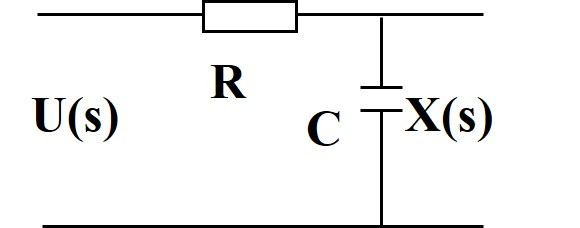
\includegraphics[width=0.34\textwidth]{fig_3_07}\\
  \caption{一阶滞后滤波}\label{fig_3_07}
\end{figure}


\begin{remark}
  一阶滞后滤波法

  优点:对周期性干扰具有良好的抑制作用,适用于波动频率较高的场合。

  缺点: 相位滞后,灵敏度低,滞后程度取决于a值大小,不能消除滤波频率高于采样频率的1/2的干扰信号。
\end{remark}

\subsection{复合数字滤波}

复合滤波就是把两种以上的滤波方法结合起来使用。例如把中值滤波的思想与算术平均的方法结合起来,就是一种常用的复合滤波法。具体方法是首先将采样值按大小排队,去掉最大和最小的,然后再把剩下的取平均值。这样显然比单纯的平均值滤波的效果要好。


例:一阶滞后滤波加上算术平均值滤波的复合滤波子程序,流程图如图\ref{fig_3_08}所示。其中,主程序初始化中已对X、S和a初始化。

\begin{figure}
  \centering
  % Requires \usepackage{graphicx}
  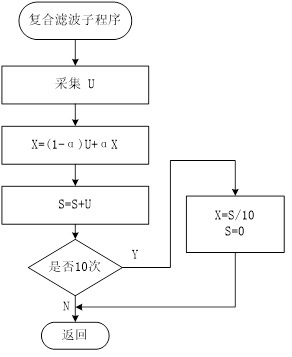
\includegraphics[width=0.45\textwidth]{fig_3_08}\\
  \caption{复合滤波器}\label{fig_3_08}
\end{figure}




\section{本章要点总结}


\begin{itemize}
  \item 什么是线性化处理?线性化方法有几种?

  \item 理解标度变换;

  \item 了解超限报警的类型和方法;

  \item 数字滤波的特点,有几种常用的数字滤波方法?各有何特点?

\end{itemize}


\chapter{抗干扰技术}

所谓干扰,就是各种噪声或造成计算机系统、设备不能正常工作的破坏因素。
干扰在工业现场普遍存在,影响系统的可靠性和稳定性,给系统调试和运行增加了难度。
要做到抗干扰,就要首先了解干扰的来源、传播途径和作用形式。




\section{干扰的来源和传播途径}


\subsection{干扰的来源}

微机控制系统所受到的干扰源分为外部干扰和内部干扰。从机理上看,内外部干扰物理性质相同,因而消除或抑制方法没有本质上的区别


\begin{description}
  \item[外部干扰]
       外部干扰的主要有:分为三类,即电源干扰、空间干扰、设备干扰。
  \item[内部干扰]
       内部干扰主要有:分布电容或分布电感产生的干扰、多点接地造成的电位差给系统带来的影响等。
\end{description}



\subsection{干扰的作用途径}


\begin{description}
  \item[静电耦合]
  干扰信号通过分布电容进行传递称为静电耦合。系统内部各导线之间,印刷线路板的各线条之间,变压器线匝之间的绕组之间以及元件之间、元件与导线之间都存在着分布电容。具有一定频率的干扰信号通过这些分布电容提供的电抗通道穿行,对系统形成干扰。

\begin{figure}[h]
  \centering
  % Requires \usepackage{graphicx}
  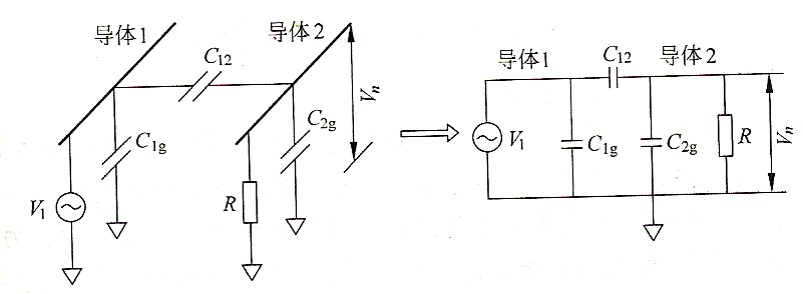
\includegraphics[height=4cm]{fig_4_01.jpg}\\
  \caption{电容耦合}\label{fig_4_01}
\end{figure}

\begin{remark}
对于图\ref{fig_4_01}
\begin{equation}
  V_n=\frac{j\omega RC_{12}}{1+j\omega R(C_{12}+C_{2g})}V_1
\end{equation}
式中起决定作用的是$R$, $C_{12}$, $C_{2g}$和频率$\omega$。分两种情况考虑频率影响:
\begin{equation}
\omega\downarrow\Rightarrow j\omega R(C_{12}+C_{2g})\ll 1 \Rightarrow V_n\ll V_1
\end{equation}
\begin{equation}
\omega\uparrow\Rightarrow j\omega RC_{12}\gg 1 \Rightarrow V_n\approx \frac{
C_{12}}{C_{12}+C_{2g}}V_1
\end{equation}
同样,式中的其它参数也会对结果产生重要影响。
\end{remark}



  \item[电磁耦合]
  电磁耦合是指在空间磁场中电路之间的互感耦合。因为任何载流导体都会在周围的空间产生磁场,而交变磁场又会在周围的闭合电路中产生感应电势,所以这种电磁耦合总是存在的,只是程度强弱不同而已。


\begin{figure}[h]
  \centering
  % Requires \usepackage{graphicx}
  \includegraphics[height=4cm]{fig_4_02.jpg}\\
  \caption{电感耦合}\label{fig_4_02}
\end{figure}

\begin{remark}
对于图\ref{fig_4_02}
\begin{equation}
  V_n=j\omega MI_1
\end{equation}
天津广播电台的地址是和平区卫津路143号,与天津大学相望。大功率广播电台会有较强的电磁辐射,对精密仪器电路产生影响。
\end{remark}

\begin{remark}
叠加定理:在线性电路中,任一支路的电压与电流,都是各个独立源单独作用下,在该支路中产生的电压与电流的代数之和。
\end{remark}

  \item[公共阻抗耦合]
  公共阻抗耦合是指多个电路的电流流经同一公共阻抗时所产生的相互影响。例如系统中往往是多个电路共用一个电源,各电路的电流都流经电源内阻和线路电阻,成为各电路的公共阻抗。每一个电路的电流在公共阻抗上造成的压降都将成为其它电路的干扰信号。

\begin{figure}[h]
  \centering
  % Requires \usepackage{graphicx}
  \includegraphics[height=4cm]{fig_4_03.jpg}\\
  \caption{公共阻抗耦合}\label{fig_4_03}
\end{figure}

\begin{remark}
汇流线路不可能是理想的导线($R=0, L=0, C=\infty $)。
如果数字电路与模拟电路部分不是分别接地,则数字电路中的高频信号会通过公共阻抗耦合到模拟电路部分,如图\ref{fig_4_03}(a,b)所示。因而,一般电路中二者分别接地,如图\ref{fig_4_03}(c)所示。
\end{remark}

\end{description}





\subsection{干扰的作用形式 }

各种干扰信号通过不同的耦合方式进入系统后,按照对系统的作用形式又可分为共模干扰、串模干扰和长线传输干扰。
\begin{description}
  \item[共模干扰]
  共模干扰是在电路输入端相对公共接地点同时出现的干扰,也称为共态干扰、对地干扰、纵向干扰、同向干扰等。共模干扰主要是由电源的地、放大器的地以及信号源的地之间的传输线上电压降造成的,如图\ref{fig_4_04}所示。
  \begin{figure}[h]
  \centering
  % Requires \usepackage{graphicx}
  \includegraphics[height=4cm]{fig_4_04.jpg}\\
  \caption{共模干扰}\label{fig_4_04}
\end{figure}



\begin{figure}[h]
  \centering
  % Requires \usepackage{graphicx}
  \includegraphics[height=4cm]{fig_4_05.jpg}(a)
  \includegraphics[height=4cm]{fig_4_06.jpg}(b)\\
  \caption{共模干扰的作用形式,(a) 单端输入, (b) 双端输入.}\label{fig_4_05}
\end{figure}


\begin{remark}
共模电压对放大器的影响,实际上是转换成串模干扰的形式而加入到放大器的输入端。

当放大器为单端输入时,如图\ref{fig_4_05}(a) 所示,共模电压Vc 引入放大器输入端的串模干扰电压为:
\begin{equation}
  V_{n1}=I_cZ_s = \frac{Z_s}{Z_s+Z_r}V_c
\end{equation}
其中,$Z_s$ 为信号源内阻;$Z_c$ 放大器输入阻抗。

因为$Z_r\gg Z_s$,得到:
\begin{equation}
  V_{n1}\approx \frac{Z_s}{Z_r}V_c
\end{equation}

如图\ref{fig_4_05}(b) 所示,当放大器为双端输入时,共模电压引入放大器输入端的串模干扰电压为:
\begin{equation}
  V_{n2} = I_{c1}Z_{s1} - I_{c2}Z_{s2} = V_cZ_{s1}/(Z_{s1}+Z_{r1}) - V_{c}Z_{s2}/ (Z_{s2}+Z_{r2})
\end{equation}
其中,Zs1、Zs2为信号源内阻;Zc1、Zc2 为放大器输入端对地的漏阻抗。

因为$Z_{c1} \gg Z_{s1}$, $Z_{c2}\gg Z_{s2}$,

所以$V_{n2} \approx V_c( Z_{s1} / Z_{c1} - Z_{s2} / Z_{c2} )$

当 $Z_{s1} / Z_{c1} = Z_{s2} / Z_{c2}$时,有$V_{n2} = 0$

\end{remark}



  \item[串模干扰]��
  串模干扰就是指串联叠加在工作信号上的干扰,也称之为正态干扰、常态干扰、横向干扰等。
  \item[长线传输干扰]��
  所谓“长线”,取决于集成电路的运算速度。例如,对于毫微秒级的数字电路来说,1米左右的连线就可以当作长线。
  长线传输的三个问题:一是长线传输易受到外界干扰,二是具有信号延时,三是高速变化的信号在长线传输时,还会出现波反射现象。
\end{description}




\section{硬件抗干扰技术}

针对前述噪声的三种作用形式,给出相应的抑制方法。

\subsection{共模干扰的抑制}
抑制共模干扰的主要方法是设法消除不同接地点之间的电位差。
\begin{description}
  \item[变压器隔离] 如图\ref{fig_4_07}所示,利用变压器把模拟电路与数字电路隔离开,也就是把模拟地与数字地断开,以使共模干扰电压无法构成回路,从而抑制共模干扰。注意:隔离变压器的前端和后端电路应当分别采用两组互相独立的电源,切断两部分的地线联系。
\begin{figure}[h]
  \centering
  % Requires \usepackage{graphicx}
  \includegraphics[width=0.4\textwidth]{fig_4_07.jpg}\\(a)\\
  \includegraphics[width=0.6\textwidth]{fig_4_07a.jpg}\\(b)\\
  \caption{变压器隔离}\label{fig_4_07}
\end{figure}

\begin{remark}
变压器隔离可以提供主边到副边之间的隔离,对直流的隔离效果尤其明显。其作用体现在:
\begin{enumerate}
  \item 隔离接地环路;
  \item 电路单元间传输的信号电流只在变压器绕组连线内流过,不流经地线,因此也可以避免对其他电路的干扰。
\end{enumerate}


\end{remark}

  \item[光电隔离]
  如图\ref{fig_4_08}所示,模拟信号经放大后,再利用光电隔离的线性区,直接对模拟信号进行光电耦合传送。


\begin{figure}[h]
  \centering
  % Requires \usepackage{graphicx}
  \includegraphics[width=0.4\textwidth]{fig_4_08.jpg}\\
  \caption{光电隔离}\label{fig_4_08}
\end{figure}

  \begin{remark}
  光电耦合具有以下特点:
  \begin{enumerate}
    \item 密封在管壳内,不受外界光的影响;
    \item 靠光传输信号,切断了各电路之间地线的联系;
    \item 其发光二极管只有通过一定的电流时才能发光,从而有效的抑制干扰信号。
  \end{enumerate}
  \end{remark}


  \item[浮地屏蔽]
  采用浮地输入双层屏蔽放大器来抑制共模干扰。所谓浮地,就是利用屏蔽方法使信号的“模拟地”浮空,从而达到抑制共模干扰的目的。
  计算机部分采用内外两层屏蔽,且内屏蔽层对外屏蔽层(机壳地) 是浮地的,而内层与信号源及信号线屏蔽层是在信号端单点接地的,被测信号到控制系统中的放大器是采用双端差动输入方式。

\begin{figure}[h]
  \centering
  % Requires \usepackage{graphicx}
  \includegraphics[width=0.6\textwidth]{fig_4_09.jpg}\\
  \caption{浮地屏蔽}\label{fig_4_09}
\end{figure}

  \begin{remark}
  图\ref{fig_4_09}中,Zs1、Zs2为信号源内阻及信号引线电阻,Zs3 为信号线的屏蔽电阻,它们至多只有十几欧姆左右,Zc1、Zc2为放大器输入端对内屏蔽层的漏阻抗,Zc3为内屏蔽层与外屏蔽层之间的漏阻抗。工程设计中Zc1、Zc2、Zc3应达到10兆欧姆以上。
  \end{remark}

  \begin{remark}
  电路分析时,可以分步进行:

  \textbf{第1步}:注意到红线框内的等效电阻Zs 必然满足:$Z_s<Z_{s3}$。 考虑Zs、Zc3与Ucm构成的回路,由于$Z_s \ll Z_{c3}$ ,可知Zs上分得的Ucm信号已被衰减到很小,即
  \begin{equation}
    U_s = U_{cm}\frac{Z_s}{Z_{c3}+Z_s}\ll U_{cm}
  \end{equation}

\textbf{第2步}:可参考对图\ref{fig_4_05}(b) 的分析过程。Us分别在Zs2 与Zs1 上的分压Us2 与Us1 进一步衰减;两个信号加到运放的差动输入端,被再次相减,衰减到很小的共模干扰信号。因而,最终能够进入计算机系统内的共模电压理论上为零。

  \end{remark}

  \item[仪表放大器]
  仪表放大器具有共模抑制能力强、输入阻抗高、漂移低、增益可调等优点,是一种专门用来分离共模干扰与有用信号的器件。
\end{description}

\subsection{串模干扰的抑制}
对于串模干扰的抑制比较困难。
\begin{description}
  \item[滤波]
    如果串模干扰频率比被测信号频率高,则采用输入低通滤波器来抑制高频串模干扰;如果串模干扰频率比被测信号频率低,则采用高通滤波器来抑制低频串模干扰;如果串模干扰频率落在被测信号频谱的两侧,应采用带通滤波器。
   一般情况下,串模干扰均比被测信号变化快,故常用二阶阻容低通滤波网络作为模/数转换器的输入滤波器。
  \item[采用双绞线作为信号线]
    若串模干扰和被测信号的频率相当,则很难用滤波的方法消除。此时,必须采用其它措施,消除干扰源。通常可在信号源到计算机之间选用带屏蔽层的双绞线或同轴电缆,并确保接地正确可靠。
    采用双绞线作为信号引线的目的是减少电磁干扰。双绞线能使各个小环路的感应电势相互抵消。一般双绞线的节距越小抗干扰能力越强。

\begin{figure}[h]
  \centering
  % Requires \usepackage{graphicx}
  \includegraphics[height=3cm]{fig_4_10.jpg}\\
  \caption{双绞线}\label{fig_4_10}
\end{figure}

\begin{figure}[h]
  \centering
  % Requires \usepackage{graphicx}
  \includegraphics[height=5cm]{fig_4_11.jpg}\\
  \caption{双绞线的节距与噪声衰减率}\label{fig_4_11}
\end{figure}



  \item[电流传送]
    当传感器信号距离主机很远时很容易引入干扰。如果在传感器出口处将被测信号由电压转换为电流,以电流形式传送信号,将大大提高信噪比,从而提高传输过程中的抗干扰能力。
\begin{remark}
\textit{
4-20mA信号指定时考虑了在多方面使用的要求:
\begin{enumerate}
  \item 30V 电压 30mA 电流 所引起的火花是可以点燃危险气体平均下限,为了保险起见,同时参照其它传统设定,所以将许多仪表定为24V供电,同时限定电流小于30mA,为了留有余地,信号上限定为 20mA。
  \item 为了区分没有信号,和信号为零,信号的起始值(信号零位值)不能为零(电气值)。
  \item 两线制仪表在信号值为零时仍需要一定的能量供应,在24V供电条件下,4mA电流提供的能量,是当时制定标准时,大部分仪表生产商能接受的能量供应下限。
  \item 4-20mA电流作用在250欧姆电阻上正好符合标准信号的电压标准 1-5V。
\end{enumerate}
上面几个条件经过整合,形成一套信号标准,包括:
24V直流供电、250欧姆标准负载、1-5V 或 4-20mA 标准信号。}
\end{remark}
\end{description}


\subsection{长线传输干扰的抑制}


采用带有屏蔽的双绞线可以在很大程度上减少空间电磁场的干扰;采用终端阻抗匹配或始端阻抗匹配,可以消除长线传输中的波反射或者把它抑制到最低限度。

\begin{description}
  \item[波阻抗的测量] 为进行阻抗匹配,必先知道长传输线的波阻抗Rp。波阻抗的测量如图\ref{fig_4_12}所示。调节电阻并用示波器观察电路A 的波形,当达到完全匹配时,即R=Rp 时,电路A输出的波形不畸变,反射波完全消失。此时的R为该线的波阻抗。

\begin{remark}
  一般双绞线的波阻抗在100-200欧姆,绞节距愈短,波阻抗愈低。同轴电缆的波阻抗一般在50-100欧姆。根据传输线的基本理论,无损耗导线的波阻抗为
  \begin{equation}
    R_p=\sqrt{\frac{L_0}{C_0}}
  \end{equation}
\end{remark}

\begin{figure}[h]
  \centering
  % Requires \usepackage{graphicx}
  \includegraphics[height=2cm]{fig_4_12.jpg}\\
  \caption{波阻抗的测量}\label{fig_4_12}
\end{figure}
  \item[波阻抗的终端匹配]
  最简单的终端阻抗匹配方法如图\ref{fig_4_13}(a)所示,其中R=Rp。

\begin{figure}[h]
  \centering
  % Requires \usepackage{graphicx}
  \includegraphics[height=5cm]{fig_4_13.jpg}\\
  \caption{长线传输中波阻抗的终端匹配}\label{fig_4_13}
\end{figure}

  \begin{remark}

由于R的存在加大了负载,使得信号波形电平下降,影响其对高电平的抗干扰能力。为此,可采用图\ref{fig_4_13}(b)所示的方法。注意其等效电阻R为:
\begin{equation}
  R=\frac{R_1R_2}{R_1+R_2}
\end{equation}
使其满足R=Rp。
  \end{remark}

  \item[波阻抗的始端匹配]

  在传输线的始端接入电阻R,也可消除波反射现象,如图\ref{fig_4_14}所示。
\begin{figure}[h]
  \centering
  % Requires \usepackage{graphicx}
  \includegraphics[height=2cm]{fig_4_14.jpg}\\
  \caption{长线传输中波阻抗的始端匹配}\label{fig_4_14}
\end{figure}

\begin{remark}
选择R时应满足:
\begin{equation}
  R=R_p-R_{src}
\end{equation}

\end{remark}


\end{description}


\section{软件抗干扰技术}
\subsection{输入/输出软件抗干扰措施}

\begin{description}
  \item[开关量(数字量)信号输入抗干扰措施]
�ザ杂诳�关量的输入,为了确保信息准确无误,在软件上可采取多次读取的方法(至少读两次),认为无误后再行输入,如图\ref{fig_4_15}示。
\begin{figure}[h]
  \centering
  % Requires \usepackage{graphicx}
  \includegraphics[height=5cm]{fig_4_15.jpg}\\
  \caption{输入抗干扰}\label{fig_4_15}
\end{figure}


  \item[开关量(数字量)信号输出抗干扰措施]     当计算机输出开关量控制闸门、料斗等执行机构动作时,为了防止这些执行机构由于外界干扰而误动作,比如已关的闸门、料斗可能中途打开;已开的闸门、料斗可能中途突然关闭。对于这些误动作,可以在应用程序中每隔一段时间(比如几个ms) 发出一次输出命令,不断地关闭闸门或者开闸门。这样,就可以较好地消除由于扰动而引起的误动作(开或关)。
\end{description}


\begin{remark}

在某个输出口上输出一个高电平去驱动一个外部器件,你如果只送一次“1”,那么,当干扰来临时,这个“1”就有可能变成“0”了。正确的处理方式是,你定期刷新这个“1”。那么,即使偶然受了干扰,它也能恢复回来。除了I/O口动作的冗余。同时也建议大家在下面各方面也采用这种方法:

1、LCD的显示。有时,也许你会用一些LCD的专用驱动芯片(如HT1621),这种芯片有个好处,即你只要将显示数据传送给它,它就会不断的自动扫描LCD。但是,你千万不要以为这样就没你啥事了。正确的处理方式是,要记得定期刷新送显数据(即使显示内容没有改变)。对于CPU中自带LCD DRIVER 的,也要定期刷新LCD RAM。

2、中断使能标志的设置。不要以为你在程序初始化段将中断设置好就OK了。应该在主程序中适当的地方定期刷新一下,以免你的中断被挂起来。

3、其它一些标志字和参数寄存器(包括你自己定义的),也要记得常常刷新。

4、其它一些你认为有必要的地方。
\end{remark}


\subsection{软件冗余技术}

程序正常运行时,程序计数器PC始终指向正在执行的这条指令的下一条指令的第一个字节的程序存储器单元地址,这样就保证了单片机能够正确地读取每一条指令的各个字节,即CPU先读取操作码,再读取操作数(如果有操作数字节的话)。在MCS51系列单片机中,程序计数器PC的寻址范围是0000H~FFFFH, 共64KB。用户应用程序中,根据系统要求,规定了程序运行的惟一路径。这体现在系统上电后,程序计数器PC有唯一的变化历程,保证了程序正常、有序地运行。程序跑飞是指系统受到某种干扰后,程序计数器PC的值偏离了给定的唯一变化历程,导致程序运行偏离正常的运行路径。程序跑飞因素及后果往往是不可预计的。

在很多情况下,程序跑飞后系统会进入死循环而导致死机。这时,
应采取有效措施引导跑飞的程序尽快退出死循环并迅速复位。实践证明,软件陷阱技术能有效引导跑飞的程序尽快退出死循环并迅速复位。


当单片机应用系统的CPU受到干扰时,不良影响的主要形式有:

\begin{enumerate}
  \item 非正常修改程序计数器PC指针;
  \item 改写可编程输出端口的状态;
  \item 非正常修改重要数据区的数据。
\end{enumerate}

以上三个方面的不良影响会使单片机应用系统程序失控,控制状态失灵,其后果是非常严重的,它甚至会使系统崩溃,造成严重的工业事故。

\begin{description}
  \item[数据冗余]     数据冗余就是将要保护的原始数据在另外两个区域同时存放,建立两个备份,当原始数据块被破坏时,用备份数据块去修复。备份数据的存放地址应远离原始的存放地址以免被同时破坏。数据区也不要靠近栈区,以防止万一堆栈溢出而冲掉数据。
\begin{remark}
  所谓数据冗余,就是:

  1、将重要的数据信息备份2份(或以上)并存放在RAM中不同的区域(指地址不相连)。

  2、当平时对这些数据进行修改时,同时也更新备份。

  3、当干扰发生并被拦截到“程序错误处理段”中时,将数据与备份做比较,采用表决方式(少数服从多数)选出正确(或可能正确?)的那个。

  4、备份越多,效果越好。(当然,你得有足够的存储空间)。

  5、只备份最最原始的数据。中间变量(指那些可以从原始数据重新推导出来的数据)不必备份。

注:

  这种思路的理论依据,源于“概率论”,即所有数据备份同时毁坏的概率是远小于其中任一备份单独损坏的概率。
\end{remark}
  \item[指令冗余]    当CPU受到干扰后,往往将一些操作数当作指令码来执行,引起程序混乱。当程序弹飞到某一单字节指令上时,便自动纳入正轨。当弹飞到某一双字节指令上时,有可能落到其操作数上,从而继续出错。当程序弹飞到三字节指令上时,因它有两个操作数,继续出错的机会更大。因此,我们应多采用单字节指令,并在关键的地方人为地插入一些单字节指令(NOP)或将有效单字节指令重复书写,这便是指令冗余。

\end{description}


\subsection{程序运行失常的软件抗干扰}

\begin{description}
  \item[设置软件陷阱]     当干扰导致程序计数器PC值混乱时,可能造成CPU离开正确的指令顺序而跑飞到非程序区去执行一些无意义地址中的内容,或进入数据区,把数据当作操作码来执行,使整个工作紊乱,系统失控。针对这种情况,可以在非程序区设置陷阱,一旦程序飞到非程序区,很快进入陷阱,然后强迫程序由陷阱进入初始状态。
    所谓软件陷阱,就是一条引导指令,强行将捕获的程序引向一个指定的地址,在那里有一段专门对程序出错处理的程序。

    软件陷阱安排在以下4 种地方:

    \begin{enumerate}
      \item 未使用的中断向量区
      \item 未使用的大片ROM空间
      \item 表格
      \item 程序区
    \end{enumerate}
\begin{remark}
  当CPU受到外界干扰,有时PC指针会飞到另一段程序中,或跳到空白段去。其实,如果PC指针飞到空白段去,倒也好处理。只要在空白段设立软件陷阱(拦截指令),将程序拦截到初始化段或程序错误处理段。

\begin{verbatim}
NOP
NOP
LJMP ERR
\end{verbatim}

\end{remark}

  \item[设置监视跟踪定时器] 也称为看门狗定时器(Watchdog),可以使陷入“死机”的系统产生复位,重新启动程序运行。这是目前用于监视跟踪程序运行是否正常的最有效的方法之一,近来得到了广泛的应用。
    在程序运行的每个循环周期内,对定时器重新初始化。如果程序运行失常,跑飞或进入局部死循环,不能按正常循环路线运行,则Watchdog定时器得不到及时的重新初始化而使定时时间到,引起复位。一般而言,控制程序具备以下基本结构:

\begin{verbatim}
void main()
{
    init();     %初始化
    while(1)
        loop(); %主循环
}
\end{verbatim}



\begin{remark}
程序正常运行时,loop()具有确定的运行周期Ta;而程序出现异常时,loop()的周期性被打乱。由此,可以判断系统程序是否正常。


\end{remark}


\begin{remark}
思考:如何利用这一特点来监控/管理CPU的运行状态呢?



看门狗的主体是一个定时器。其功能为:每隔一定周期Tc产生一个定时器溢出;如在定时器溢出前对其清零,则重新计时。

在loop()中加入指令,可周期性(Ta)的清零看门狗定时器。这一操作,称为“喂狗”。注意:Tc略大于Ta。以下分两种情况分析:

\begin{enumerate}
  \item 当程序正常运行时,loop()中的这一条指令能够定时“喂狗”,则狗儿不叫,定时器不会溢出;
  \item 而当程序出现异常时,loop()中的喂狗指令不会被运行,没有喂狗,则狗儿会叫,定时器会溢出;
\end{enumerate}

定时器溢出,可用于触发对CPU的复位或NMI,使CPU程序能够恢复正常运行。

\end{remark}

\begin{remark}

看门狗可分为硬件看门狗和软件看门狗两种。


软件看门狗原理上一样,只是将硬件电路上的定时器用处理器的内部定时器代替。这样可以简化硬件电路设计,但在可靠性方面不如硬件定时器,比如系统内部定时器自身发生故障就无法检测到。当然也有通过双定时器相互监视,这不仅加大系统开销,也不能解决全部问题,比如中断系统故障导致定时器中断失效。

看门狗本身不是用来解决系统出现的问题,在调试过程中发现的故障应该要查改设计本身的错误。加入看门狗目的是对一些程序潜在错误和恶劣环境干扰等因素导致系统死机而在无人干预情况下自动恢复系统正常工作状态。看门狗也不能完全避免故障造成的损失,毕竟从发现故障到系统复位恢复正常这段时间内是不能正常工作的。同时一些系统也需要复位前保护现场数据,重启后恢复现场数据,这可能也需要一笔软硬件的开销。
\end{remark}

\end{description}

\begin{figure}[h]
  \centering
  % Requires \usepackage{graphicx}
  \includegraphics[width=0.4\textwidth]{fig_4_16.jpg}\\
  \includegraphics[width=0.7\textwidth]{fig_4_16a.jpg}
  \caption{MAX1232 连接及管脚定义}\label{fig_4_16}
\end{figure}




\subsection{其他手段}

\begin{enumerate}
  \item 分散结构设计

把整体的软件设计分散成各子系统的设计,各自独立,又共享资源。
\item 容错技术

在软件设计中的容错技术是指在软件设计时,对误操作不予响应的技术。基本活动有四种:故障检测、损坏估计、故障恢复和缺陷处理。
\item 标准化

采用标准化的软件可以提高软件运行的可靠性。

\end{enumerate}





\section{供电与接地技术}


\subsection{供电技术}
电网的干扰,频率的波动将直接影响系统的可靠性与稳定性。考虑采取电源保护措施,防止电源干扰,并保证不间断地供电。

\subsubsection{交流电源系统}

供电系统的一般保护,如图\ref{fig_4_17} 所示。

(1)选用供电比较稳定的进线电源;

(2)利用干扰抑制器消除尖峰干扰;

(3)采用交流稳压器稳定电网电源。
\begin{figure}[h]
  \centering
  % Requires \usepackage{graphicx}
  \includegraphics[width=0.5\textwidth]{fig_4_17}\\
  \caption{交流电源系统}\label{fig_4_17}
\end{figure}




\subsubsection{直流电源系统}

供电系统的一般保护,如图\ref{fig_4_18} 所示。

(1)交流电源变压器的屏蔽;

(2)采用直流开关电源;

(3)直流供电系统的隔离。

\begin{figure}[h]
  \centering
  % Requires \usepackage{graphicx}
  \includegraphics[width=0.6\textwidth]{fig_4_18}\\
  \caption{直流电源系统}\label{fig_4_18}
\end{figure}



\subsection{接地技术}


\subsubsection{地线系统的分析}

  地线的分类:
\begin{enumerate}
\item 模拟地:它是放大器,A/D,D/A转换器中的模拟电路零电位。
\item 数字地:各种数字电路的零电位。
\item 安全地:目的是使设备机壳与大地等电位,以避免机壳带电而影响人身及设备的安全(通常又称为保护地或机壳地);
\item 系统地:上述几种地的最终汇流点,直接与大地相连;
\item 交流地:交流50Hz电源的地线,它是噪声地。
\end{enumerate}


\subsubsection{主机系统的接地}

根据接地理论,低频电路(频率小于1MHz) 应单点接地,高频电路(频率大于10MHz)应就近多点接地。介于低频与高频之间时,单点接地的地线长度不得超过波长的1/20,否则应采用多点接地。


\subsubsection{接地方式}

\begin{enumerate}



\item 单点接地如图\ref{fig_4_19}所示,包括:

\begin{description}
    \item[串联接地] 各电路间相互会发生干扰, 适用各电路的电平相差不大.
    \item[并联接地] 不会因地电流而引起各电路间的耦合,其缺点是需要连很多根地线。
\end{description}


\begin{figure}[h]
  \centering
  % Requires \usepackage{graphicx}
  \includegraphics[width=0.6\textwidth]{fig_4_19}\\
  \caption{单点接地}\label{fig_4_19}
\end{figure}


\item 汇流法单点接地,如图\ref{fig_4_20}所示:


\begin{figure}[h]
  \centering
  % Requires \usepackage{graphicx}
  \includegraphics[width=0.35\textwidth]{fig_4_20}\\
  \caption{汇流法接地}\label{fig_4_20}
\end{figure}



\item 输入通道的接地技术,如图\ref{fig_4_21}所示,包括:

\begin{description}
  \item[电路一点地基准]
信号源端接地时,放大器电源不接地;放大器接地时,信号源不接地。
  \item[电缆屏蔽层的接地] 信号电路一点接地时,低频电缆的屏蔽层也一点接地。
\end{description}


\begin{figure}[h]
  \centering
  % Requires \usepackage{graphicx}
  \includegraphics[width=0.5\textwidth]{fig_4_21}\\
  \caption{输入通道的接地}\label{fig_4_21}
\end{figure}

\item 多机一点接地,如图\ref{fig_4_22}(a)所示:

\begin{figure}[h]
  \centering
  % Requires \usepackage{graphicx}
  \includegraphics[width=0.5\textwidth]{fig_4_22}(a)
  \includegraphics[width=0.3\textwidth]{fig_4_23}(b)\\
  \caption{(a)多机一点接地, (b)主机外壳接地及机芯浮空}\label{fig_4_22}
\end{figure}



\item 主机外壳接地及机芯浮空,如图\ref{fig_4_22}(b)所示:



\end{enumerate}


\section{本章要点总结}

\begin{itemize}

\item 了解干扰的来源和传播途径;
\item 了解硬件抗干扰的常用方法;
\item 了解输入/输出软件抗干扰措施、软件冗余以及程序运行失常的软件抗干扰 ;
\item 了解接地系统以及不同的接地技术;

\end{itemize}

\setcounter{chapter}{4}
\chapter{数据通信技术基础}

数据通信是随着计算机技术与通信技术的迅速发展,以及两者间的相互渗透与结合而兴起的一种新的通信方式。在工业控制领域,随着工业生产规模的扩大和自动化水平的提高,越来越多的数据共享和消息交换需要通过数据通信解决。计算机控制系统中的数据通信指计算机与计算机之前间、计算机与仪器设备之间的数据交换。


\section{通信系统的性能指标}

通信系统的任务是传递信息,因而信息传输的有效性和可靠性是通信系统最主要的质量指标。


通信系统的模型为:


信息源 $\rightarrow d(t)$ 发送器 $\rightarrow s(t)$ 传输通道 $\rightarrow r(t)$  接收器 $\rightarrow d'(t)$  汇

\begin{remark}
由此模型可考虑以下问题:

\begin{enumerate}
  \item 接收到的数据d'(t)是否d(t)?
  \item 发送器及接收器的作用?具体是什么?
  \item 传输通道的具体形式?
  \item 如何衡量通信系统的性能?
\end{enumerate}

\end{remark}

\subsection{有效性指标}

\subsubsection{数据传输速率}

 包含以下两种:
  \begin{enumerate}
    \item 比特率

比特是数据信号的最小单位。
    通信系统每秒传输数据的二进制位数定义为比特率,记作bps。
    \item 波特率

波特是指信号大小方向变化的一个波形;把每秒传输信号的个数定义为波特率。
    单位: 波特(baud)。
  \end{enumerate}

\begin{remark}

波特率表示单位时间内信号波形的变换次数,即通过信道传输的码元个数。
若信号码元宽度为T秒,则码元速率B=1/T,单位叫波特。这是为了纪念电报码的发明者法国人波特(Baudot)。

1924年奈奎斯特推导出有限带宽无噪声信道的极限波特率,称为奈氏定理。若信道带宽为W,则奈氏定理的最大码元速率为:$B=2W (Baud)$

奈氏定理指定的信道容量也叫奈氏极限,它由信道的物理特性决定。超过奈氏极限传送脉冲信号是不可能的。因此要进一步提高波特率,就必须改善信道的带宽。

比特率指单位时间内信道上传送的信息量(比特数)。数字信道的通频带(即带宽)决定了信道中能不失真的传输脉冲序列的最高速率,即信道容量。在一定波特率下提高比特率的途径是让一个码元携带更多的信息量(比特数)。若把两比特编码为一码元,则数据速率可成倍提高,我们有公式:

\begin{equation}
R=Blog_2N=2Wlog_2N
\end{equation}

式中R表示比特率,B、N、W的含义如上所述,单位为每秒比特(bits per second),记为bps或b/s。

\end{remark}





  \begin{remark}

例如,有一个带宽为3kHz的理想低通信道,其码元传输速率为6000baud。而最高数据速率可随编码方式的不同而有不同的取值。若1 个码元能携带2bit的信息量,则最高的数据速率为12000bps。这些都是不考虑噪声的理想情况下的极限值。至于有噪声影响的实际信道,则远远达不到这个极限值。

  \end{remark}


  \subsubsection{协议效率}

协议效率是指所传输的数据包中的有效数据位与整个数据包长度的比值。通常用百分比表示。

  协议效率越高,其通信的有效性越好。
   通信参考模型的每个分层,都会有相应的层管理和协议控制的加码。从提高协议效率的角度来看,减少层次可以提高编码效率。


\subsection{可靠性指标}

  \textbf{误码率}是衡量数字通信系统可靠性的指标,是二进制码元在数据传输系统中被传错的概率,数值上近似:

  \begin{equation}
    P_e\approx N_e/N
  \end{equation}

N:传输的二进制码元总数;
Ne:为传输错的码元数

   \begin{remark}
     理解误码率应注意以下问题:
     \begin{enumerate}
       \item 误码率是衡量数据传输系统正常工作状态下传输可靠性的参数;
       \item 对于一个实际的数据传输系统,不能笼统的说误码率越低越好,要根据实际情况提出误码率要求;
       \item 实际数据传输中,往往需要进行大量的、重复的测试,才能求出平均误码率。
     \end{enumerate}


         据测试,电话线传输速率为$300-2400bps$时,平均误码率为$10^{-4} - 10^{-6}$,而计算机通信的平均误码率要求低于$10^{-8}$,因此,不采用差错控制,就不能满足计算机通信的要求。

   \end{remark}


\section{通信线路工作方式}


如图\ref{fig_5_01}所示,
  单工通信是指所传送的信息始终朝着一个方向,而不进行相反方向的传送。
  半双工(Half Duplex)通信是指信息可双向传输,但同一时刻只限于一个方向的传输。
  全双工(Full Duplex)通信是指能够同时进行双向数据通信。




\begin{center}
\begin{figure}
  \centering
  \includegraphics[width=0.6\textwidth]{fig_5_01}\\
  \caption{工作方式}\label{fig_5_01}
\end{figure}
\end{center}

\begin{remark}
举例:

  \begin{description}
       \item[单工] 广播电台,电台,单行路
       \item[半双工] 对讲机,USB 2.0,RS-485,分时段单行路
       \item[全双工] 电话,RS-232,USB 3.0,网络端到端通信(微信,QQ),一般道路
     \end{description}


\end{remark}

\section{传输介质与介质带宽}

\subsection{传输介质}

\textbf{传输介质}指数据通信中用来传递信号的媒体。例如,双绞线,屏蔽电缆,光纤。



\begin{center}
\begin{figure}
  \centering
  \includegraphics[width=0.55\textwidth]{fig_5_02}
  \includegraphics[width=0.40\textwidth]{fig_5_03}\\
  \caption{双绞线-(STP/UTP)}\label{fig_5_03}
\end{figure}
\end{center}



\begin{center}
\begin{figure}
  \centering
  \includegraphics[width=0.6\textwidth]{fig_5_04}\\
  \caption{同轴电缆}\label{fig_5_04}
\end{figure}
\end{center}



\begin{center}
\begin{figure}
  \centering
  \includegraphics[width=0.55\textwidth]{fig_5_05}
  \includegraphics[width=0.40\textwidth]{fig_5_05a}
  \caption{光纤传送模式:MMF与SMF,单芯与多芯}\label{fig_5_05}
\end{figure}
\end{center}


\begin{remark}
光纤特点:直径小、频带宽、容量大、远距离高速传输、不受外界电磁干扰;成本相对昂贵、连接复杂
\end{remark}


\subsection{介质带宽}

不同的传输介质具有不同的带宽。


\begin{center}
\begin{figure}
  \centering
  \includegraphics[width=0.55\textwidth]{fig_5_06}\\
  \caption{电话线的带宽}\label{fig_5_06}
\end{figure}
\end{center}

\begin{remark}
以电话线为例,如图\ref{fig_5_06}所示。
\begin{description}
  \item[信号带宽] 信号频谱的宽度,即信号的最高频率分量与最低频率分量之差。
  \item[介质带宽] 限定了允许通过该传输介质的信号的上、下限频率,也即一个频率能带。
\end{description}

情形1:如果信号与介质带宽相同且频率范围一致,信号能不损失频率成分地通过信道。
情形2:如果带宽相同,但频率范围不一致,则该信号的某些频率分量肯定不能完全通过该介质。

\end{remark}

\section{基带与载波传输}

\subsection{基带传输}

\begin{description}
  \item[基带传输] 在基本不改变数据信号频率的情况下,在数字通信中直接传送数据基带信号,即按数据波的原样进行传输,不采用任何调制措施。
目前,大部分计算机局域网都是采用基带传输。特点:
\begin{itemize}
  \item 信号按数据位流的基本形式传输,整个系统不用调制解调器。
  \item 基带信号包含很宽频率范围,不适合远距离传输。
\end{itemize}

  \item[数字数据的数字编码] 用高低电平的矩形脉冲信号来表示数据的0、1状态。

  数字编码的种类有:单极性码、双极性码、归零码、非归零码、差分码、Manchester编码等。工业通信中常用的是非归零码和Manchester编码,如图\ref{fig_5_07}所示。

\end{description}

\begin{description}
  \item[非归零码] 通过高低电平表示逻辑1和0,在整个码元期间都维持有效电平的编码。

\begin{itemize}
  \item
\textbf{优点}:能够比较有效地利用信道的带宽,这是最常用的编码之一。
  \item
\textbf{缺点}:存在直流分量,不具备自同步机制,必须使用外同步。
\end{itemize}

  \item[曼彻斯特编码] 在每个码元的中间都要发生跳变。接收端可将此变化提取出来作为同步信号,使接收端的时钟与发送设备的时钟保持一致。是工业数据通信中最常用的一种基带信号编码

\begin{itemize}
  \item \textbf{优点}:不需要外同步信号,不存在直流分量。
  \item \textbf{缺点}:需要双倍的传输带宽(即信号速率是数据速率的2倍)。
\end{itemize}

\begin{center}
\begin{figure}
  \centering
  \includegraphics[width=0.55\textwidth]{fig_5_07}\\
  \caption{非归零码/曼彻斯特编码}\label{fig_5_07}
\end{figure}
\end{center}


\end{description}


\subsection{载波传输}

\begin{description}
  \item[载波传输] 是先用数字信号对载波进行调制,然后进行传输的传输模式。

  \item[基本原理] 用数字信号对载波$S(t)=Acos(\omega t+\phi)$ 的三个参量(幅度、频率、相位)进行调制,如图\ref{fig_5_08}所示。

  \item[常用技术] 包括:

  \begin{enumerate}
    \item 调幅: 幅移键控ASK(Amplitude Shift Keying)
    \item 调频: 频移键控FSK(Frequency Shift Keying)
    \item 调相: 相移键控PSK(Phase Shift Keying)
  \end{enumerate}

\begin{center}
\begin{figure}
  \centering
  \includegraphics[width=0.55\textwidth]{fig_5_08}\\
  \caption{ASK/FSK/PSK}\label{fig_5_08}
\end{figure}
\end{center}

\end{description}



\section{通信数据的差错校验}
数据通信中,由于干扰等各种原因,数据差错不可避免,需要可靠判断出传输是否有误,即\textbf{差错校验}。

差错校验的\textbf{基本原理}是:发送方在发送数据基础上,生成某些\textbf{校验编码},附加在数据后面一起发送。接收方收到数据和校验码后,用校验码进行检验,确定本次传输是否出现错误。


\begin{description}
  \item[奇偶校验] 用这种校验方法,在发送时,在每一个字符的最高位之后都附加一个奇偶校验位。这个校验位可为“1”或为“0”,以便保证整个字符(包括校验位)为“1” 的位数为偶数(偶校验)或为奇数(奇校验)。接收时,按照发送方所确定的同样的奇偶性,对接收到的每一个字符进行校验,若二者不一致,便说明出现了差错。

      \begin{remark}
        ASCII码包含128个常用字符。因此,可用7b来表示其中的一个字符。在用ASCII码传递信息时,对其进行校验,如图\ref{fig_5_12}所示。

      \end{remark}
\begin{figure}
  \centering
  \includegraphics[width=0.4\textwidth]{fig_5_12}\\
  \caption{奇偶校验举例}\label{fig_5_12}
\end{figure}

\begin{remark}
  奇偶校验如何实现?异或运算(相异为1),即:

  $b_{check} = b1\bigoplus b2 \bigoplus b3 \bigoplus b4 \bigoplus b5 \bigoplus b6 \bigoplus b7 \bigoplus b8$

  对于01010101、11111111、00000000、00000001、00000011、11111110奇偶校验码分别为?
\end{remark}

  \item[校验和] 该种校验方法是针对数据块,而不是单个字符。在数据发送时,发送方对块中数据简单求和,产生一字节校验字符(校验和)附加到数据块结尾。校验和不能检测出排序错误。
\begin{figure}
  \centering
  \includegraphics[width=0.55\textwidth]{fig_5_09}\\
  \caption{校验和}\label{fig_5_09}
\end{figure}
  \item[循环冗余码校验] CRC (cyclic redundancy code) 检错码方法是将要发送的数据序列当作一个信息多项式$f(x)$的系数,在发送方用收发双方预先约定的生成多项式G(x)去除,求得一个余数多项式R(x)。将余数多项式加到数据多项式之后发送给接收端。接收端用同样的生成多项式去除接收数据多项式$f'(x)$,得到计算余数多项式,然后进行比较。
  生成多项式由协议规定,目前已有多种生成多项式列入国际标准,如图\ref{fig_5_11}所示。

\begin{figure}
  \includegraphics[width=0.48\textwidth]{fig_5_10}
  \includegraphics[width=0.48\textwidth]{fig_5_11}\\
  \caption{循环冗余码的种类和计算}\label{fig_5_11}
\end{figure}

\begin{remark}

\begin{itemize}
  \item 数据与多项式的对应关系;
  \item 余数的长度应为多少;
  \item 如何进行模2除法;
\end{itemize}
\end{remark}

\begin{remark}
模2除法:除法过程中用到的减法是模2减法, 不考虑加法进位和减法借位。只要部分余数首位为1,便可上商1,否则上商0。

\begin{verbatim}
0-0=0   0-1=1   1-0=1   1-1=0
\end{verbatim}

\end{remark}

\begin{remark}

例:如图\ref{fig_5_13}所示


\begin{enumerate}
  \item 发送数据比特序列为110011(6比特)。
  \item 生成多项式比特序列为11001(5比特,k=4)。
  \item 将发送数据比特序列乘以$2^4$,那么产生的乘积应为1100110000。
  \item 将乘积用生成多项式比特序列去除,按模二除法应为
  \item 将余数比特序列加到乘积中得1100111001

\item 如果在数据传输过程中没有发生传输错误,那么接收端接收到的带有CRC校验码的接收数据比特序列一定能被相同的生成多项式整除,即
\end{enumerate}


\end{remark}

\begin{center}
\begin{figure}
\centering
  \includegraphics[width=0.6\textwidth]{fig_5_13}\\
  \caption{循环冗余码计算}\label{fig_5_13}
\end{figure}
\end{center}



\end{description}


\begin{remark}
  校验码的意义在于检查出错误,但并非可以$100\%$检查出错误。注意如下关系:

  校验错误 $\Rightarrow$ 数据传输错误。

  校验无误 $\Rightarrow$ 数据传输无误?

\end{remark}

\section{本章要点总结}

\begin{itemize}
  \item 数据通信的有效性和可靠性指标;

  \item 了解不同的传输介质,理解介质带宽以及其对信号传输的影响;

  \item 通信线路的工作方式;

  \item 了解信号的基带与载波传输模式,理解调制方法;

  \item 了解各种差错校验方法。

\end{itemize}

\chapter{总线技术}

总线,即一束公用信号线的集合。其定义了各引线的信号、时序、电气和机械特性,为计算机系统内部各部件、各模块间或计算机各系统之间提供了标准的公共信息通路。
总线一般有内部总线、系统总线和外部总线。
       \begin{description}
             \item[内部总线] 是计算机内部各外围芯片与处理器之间的总线,用于芯片一级的互连;
             \item[系统总线]        是微机中各插件板与系统板之间的总线,用于插件板一级的互连;

             \item[外部总线]        则是微机和外部设备之间的总线,微机作为一种设备,通过该总线和其他设备进行信息与数据交换,它用于设备一级的互连。

           \end{description}




\section{内部总线}

\subsection{I$^2$C总线}

\textbf{I$^2$C(Inter-IC)}总线10多年前由Philips公司推出,是近年来在微电子通信控制领域广泛采用的一种新型总线标准。它是同步通信的一种特殊形式,具有接口线少,控制方式简化,器件封装形式小,通信速率较高等优点。在主从通信中,可以有多个I$^2$C总线器件同时接到I$^2$C 总线上,通过地址来识别通信对象。

\subsection{SPI总线}

\textbf{串行外围设备接口SPI(serial peripheral interface)}总线技术是Motorola公司推出的一种同步串行接口。Motorola公司生产的绝大多数MCU (微控制器)都配有SPI硬件接口,如68系列MCU。SPI 总线是一种三线同步总线,因其硬件功能很强,所以,与SPI有关的软件就相当简单,使CPU有更多的时间处理其他事务 。


\section{系统总线}


\subsection{ISA总线}
IBM公司


\begin{itemize}
  \item 1981年推出基于8位机的PC/XT总线,PC总线
  \item 1984年推出基于16位机的PC/AT总线,AT总线
    但从未公开过AT总线的技术规格
\end{itemize}

Intel公司、IEEE和EISA集团联合推出ISA总线,如图\ref{fig_6_01}所示。

\begin{itemize}
  \item 与IBM/AT原装机总线意义相近的ISA(Industry Standard Architecture)总线,即8/16位的“工业标准结构”:数据传输率最高8MB/s, 寻址空间为$2^{24}=16MB$
\end{itemize}

\begin{figure}
  \centering
  % Requires \usepackage{graphicx}
  \includegraphics[width=0.6\textwidth]{fig_6_01}\\(a)\\
  \includegraphics[width=0.4\textwidth]{fig_6_01a}(b)
  \includegraphics[width=0.4\textwidth]{fig_6_01b}(c)\\
  \caption{ISA总线的IO定义及形式}\label{fig_6_01}
\end{figure}



\subsection{PCI总线}

PCI (Peripheral Component Interconnect)
\begin{itemize}
  \item 现在是主板上最常见的插槽(如下页图示)

  \item 不依附于某个具体的处理器
  \item 结构上是在CPU与原来的系统总线间插入的一级总线,具体由一个桥接电路实现对该层的管理;提供信号缓存,支持10 种外设

  \item 数据总线32/64位,最大传输速率达132MB/s

  \item 可同时支持多组外围设备

\end{itemize}

\begin{figure}
  \centering
  % Requires \usepackage{graphicx}
  \includegraphics[width=0.3\textwidth]{fig_6_02}(a)
  \includegraphics[width=0.4\textwidth]{fig_6_02a}(b)\\
  \caption{PCI总线的形式}\label{fig_6_02}
\end{figure}


\subsection{PC/104总线}


\textbf{PC/104总线}专门为嵌入式控制而定义的工控总线
实质上是一种紧凑型,小型化的 IEEE-P996. 其型号定义和PC/AT基本一致,但电气和机械规范却完全不同,是一种优化的,小型堆栈式结构的嵌入式控制系统。
PC/104总线产品软件上与PC/AT完全兼容。

\subsubsection{PC/104硬件特点:}

\begin{itemize}
  \item 小尺寸结构,标准模块:96x90mm

  \item 堆栈式,“针”“孔”总线连接,即PC/104总线模块之间总线的连接是通过上层的针和下层的孔相互咬和相连,有极好的抗震性。

  \item 4mA总线驱动既可使模块正常工作,低功耗,减少元件数量

  \item 自我堆栈式连接,无须母板

\end{itemize}

\subsubsection{PC/104版本:}
\begin{itemize}
  \item PC/104, 8位,16位分别与PC和PC/AT相对应

  \item PC/104plus则与PCI总线相对应

  \item 一个PC/104 CPU模块则可以同时拥有PC/104和PC/104plus总线

\end{itemize}


\section{外部总线}


\subsection{RS-232-C}

RS—232-C是由美国电子工业协会(EIA)制定的物理接口标准,是RS-232 标准的第3版。是一种应用非常广泛的标准总线,经1987年1月修改后,定名为RS—232-D,但两者差距不大,因此基本成为等同标准。它包括了按位串行传输的电气和机械方面的规定。适合于短距离或带调制解调器的通讯场合。

\begin{enumerate}
  \item 机械指标:标准D型25针插头或9针插头


  \item 电气特性:RS-232-C采用负逻辑,各种信号电平规定如下:

数据信号逻辑“1”:  -3v~-15v(一般用-12v)

数据信号逻辑“0”:  +3v~+15v(一般用十12v)

  \item 通信距离

  RS-232-C标准规定,驱动器可驱动2500pF的电容负载(包括传输介质和接收器输入电容),通信距离将受此电容限制,例如,普通的非屏蔽多芯电缆,每米电容值为131-164pF,因此最大通信距离2500/164≈15m;

\item 信号线定义,如图\ref{fig_6_04}所示。
\begin{figure}
  \centering
  % Requires \usepackage{graphicx}
  \includegraphics[width=0.3\textwidth]{fig_6_04} (a)
  \includegraphics[width=0.3\textwidth]{fig_6_04a} (b)\\
  \includegraphics[width=0.3\textwidth]{fig_6_04b} (c)
  \caption{RS-232信号线定义及连接方式}\label{fig_6_04}
\end{figure}

\item 常用芯片: MAX232,MAX202、MAX3232等

\item 连接方式,如图\ref{fig_6_04}(c)所示。



\end{enumerate}




\subsection{RS-485总线}

如图\ref{fig_6_05}所示,RS-485采用平衡差分电路,因此具有抑制共模干扰的能力。加上总线收发器具有高灵敏度,能检测低至200mV的电压,故传输信号能在千米以外得到恢复。

\begin{figure}
  \centering
  % Requires \usepackage{graphicx}
  \includegraphics[width=0.24\textwidth]{fig_6_05}(a)
  \includegraphics[width=0.4\textwidth]{fig_6_05a}(b)
  \caption{RS-485}\label{fig_6_05}
\end{figure}


\begin{figure}
  \centering
  % Requires \usepackage{graphicx}
  \includegraphics[width=0.4\textwidth]{fig_6_05b}
  \caption{RS-485网络拓扑结构}\label{fig_6_05a}
\end{figure}

如图\ref{fig_6_05a}所示,RS-485 最佳的网络 结构是菊花链形,不要形成很长的支干。其中,(d-f)是好的连接方式。


\begin{remark}

图中\ref{fig_6_05a}(a-c)错误之处在于:信号在各支路末端反射后与原信号迭加,造成信号质量下降。此外,还要注意总线特性阻抗的连续性,在阻抗不连续点也会发生信号的反射。例如,总线的不同区段采用不同电缆或有过长的分支线时都会出线阻抗通信质量严重下降。总之,应该提供一条单一、连续的信号通道作为总线。
\end{remark}


RS-485本身只是物理层的接口规范,只规定了物理接口的机械、电气特性,并没有对通信中的链路连接、网络控制权问题做出相关规定,因而在实际使用中,还需要自定义通信协议或与其它规范中的高层通信协议结合使用(Modbus)。一些现场总线也采用RS -485规范作为其物理层的接口标准,例如:PROFIBUS、BACnet等。


\begin{figure}
  \centering
  % Requires \usepackage{graphicx}
  \includegraphics[width=0.4\textwidth]{fig_6_06}
  \caption{RS-485报文内容}\label{fig_6_06}
\end{figure}


\subsection{IEEE-488总线}


IEEE-488是1970年由美国惠普公司开发的并行通讯总线。IEEE-488共定义了24根线(其中8根地线):

\begin{itemize}
  \item
数据总线DIO0~ DIO8
\item 数据传送控制线
\item 数据有效线DAV、未准备好接受数据线NRFD、未接受好数据线NDAC
\item 接口管理总线
\item 接口清除线IFC、服务请求线SQR、注意线ATN、结束或识别线EQI、远程允许REN

\end{itemize}

使用IEEE-488的约定:

\begin{itemize}

\item 数据传输率不得超过每秒1M字节
\item 总线上的设备数不得多于15个
\item 电缆总长度不超过20m,两设备间不超过4m
\item 采用负逻辑


\end{itemize}

\subsection{USB总线}

通用串行总线USB(universal serial bus)是由Intel、 Compaq、Digital、IBM、Microsoft、NEC、Northern Telecom等7家世界著名的计算机和通信公司共同推出的一种新型接口标准。

\begin{itemize}


\item 它基于通用连接技术,实现外设的简单快速连接,达到方便用户、降低成本、扩展PC连接外设范围的目的。
\item 使用新的、通用标准连接器,在计算机上添加设备时不必再打开机箱,安装板卡,甚至都不必重新启动,就可以使用新的设备,USB使您的计算机更易使用。

\item 可以为外设提供电源


\end{itemize}

\begin{itemize}

\item 连结的设备数:
一个USB最多可以连结127个设备

\item 传输速度:


\begin{itemize}
\item 若是使用鼠标或者键盘等不需要高速的设备时,它就采用1.5Mbps的传输速率
\item 若是使用MODEM,音箱、打印机等需要高速传输数据的设备时,则采用12Mbps的同步传输速率(结点间距离5米)。
\item USB2.0标准的MAX传输率480Mbps.


\end{itemize}

\end{itemize}

\subsection{IEEE 1394总线}

IEEE 1394是一种串行接口标准,又名Firewire“火线”,这种接口标准允许把电脑/电脑外部设备/各种家电非常简单地连接在一起。

IEEE 1394的连接电缆中共有六条芯线,其中两条线为电源线,可向被连接的设备提供电源;其它四条线被包装成两对双绞线,用来传输信号,电源的电压范围是8-40V直流电压,最大电流1.5A,像数码相机之类的一些低功耗设备可以从总线电缆内部取得电力,而不必为每一台设备配置独立的供电系统.

1394商业协会正在着手制定IEEE 1394b,这是一个在首阶段会将数据传输速率提高到1.6Gbps、而后计划提高到3.2Gbps的新版本。



\section{现场总线}


变送器、控制器、执行器等现场装置往往采用4-20mA的信号进行通讯联系,无论它们的制造厂商是谁,它们一般都可以互换。从20世纪60年代发展起来的4-20mA信号是一种国际标准,目前仍在使用。
进入20世纪80年代以来,用微处理器技术实现过程控制以及智能传感器的发展导致需要用数字信号取代4-20mA模拟信号,这就形成了现场总线。

\textbf{概念:}国际电工委员会标准IEC61158的定义:现场总线是一种应用于生产现场,在现场设备之间、现场设备与控制装置之间实行双向、串行、多节点数字通信的技术。

一般认为,现场总线是一种全数字化、双向、多站的通信系统,是用于工业控制的计算机系统的工业总线。它是用于生产自动化最底层的现场设备以及现场仪表的互联网络,是现场通信网络和控制系统的集成。

\begin{figure}
  \centering
  % Requires \usepackage{graphicx}
  \includegraphics[width=0.6\textwidth]{fig_6_07}
  \caption{OSI参考模型}\label{fig_6_07}
\end{figure}


各厂家在实际制定自己的通信协议时,并非都在产品中实现了这7层协议,而往往依据侧重点的不同,仅仅实现该7层协议的子集。



制订现场总线标准的机构

\begin{itemize}

\item IEC(国际电工委员会)

   IEC/TC65/SC65C/WG6:通过了IEC 61158标准。
   IEC/TC17/SC17B:通过了IEC62026,包括:ASI、DeviceNet、SDS 和Seriplex。


\item ISO(国际标准化组织)
      ISO11898    CAN


\end{itemize}


IEC61158标准的类型:第3版于2003年制定,包括l0种技术类型:

\begin{itemize}

\item 类型1:IEC技术报告(即相当于FF的H1,美国Fisher-Rosemount公司支持);
\item 类型2:ControlNet(美国Rockwell公司支持);
\item 类型3:Profibus(德国Siemens公司支持);
\item 类型4:P-Net(丹麦Process Data公司支持);
\item 类型5:FF HSE(High Speed Ethernet美国Fisher-Rosemount公司支持);
\item 类型6:SwiftNet(美波音公司支持);
\item 类型7:WorldFIP(法国阿尔斯通Alstom公司支持);
\item 类型8:Interbus(德国菲尼克斯Phoenix 公司支持);
\item 类型9:FF应用层(Application Layer);
\item 类型10:Profinet。
\end{itemize}


2007年 ,IEC61158现场总线标准通过,包括20个类型,如图所示。
\begin{figure}
  \centering
  % Requires \usepackage{graphicx}
  \includegraphics[width=0.6\textwidth]{fig_6_08}
  \caption{现场总线类型}\label{fig_6_08}
\end{figure}




\section{本章要点总结}

\begin{itemize}
  \item 了解各种总线的知识,重点对RS232和RS485进行理解;

  \item 理解现场总线的概念,了解几种典型的现场总线。

\end{itemize}

\chapter{计算机网络}

\section{概述}


\subsection{计算机网络的作用}

计算机网络,是指将地理位置不同的具有独立功能的多台计算机,通过通信线路连接起来,在网络通信协议的管理和协调下,实现\textbf{信息交换和资源共享}的计算机系统。


\begin{description}
  \item[信息交换] 计算机网络使上网用户之间都可以进行信息交互,好像这些用户的计算机都可以彼此直接连通一样。
  \item[资源共享] 可以是信息共享、软件共享,也可以是硬件共享。
\end{description}



\subsection{因特网概述}

因特网起源于美国,现已发展成为世界上最大的国际性计算机互联网。网络(network)由若干结点(node)和连接这些结点的链路(link) 组成。互联网是“网络的网络”(network of networks)。连接在因特网上的计算机都称为主机(host)。

网络把许多计算机连接在一起,因特网则把许多网络连接在一起,如图所示。

\begin{figure}
  \centering
  % Requires \usepackage{graphicx}
  \includegraphics[width=0.55\textwidth]{fig_7_01}
  \includegraphics[width=0.4\textwidth]{fig_7_01a}\\
  \caption{网络的网络-互联网}\label{fig_7_01}
\end{figure}


因特网发展的三个阶段:
\begin{enumerate}
  \item 第一阶段(1969-1983):单个网络 ARPANET向互联网发展的过程。

  \item 第二阶段(1983-1995):该阶段的特点是建成了三级结构(主干网、地区网和校园网)的因特网。


  \item 第三阶段(1995-至今):该阶段的特点是逐渐形成了多层次 ISP 结构的因特网。出现了因特网服务提供者 ISP (Internet Service Provider)。
\end{enumerate}


\subsection{因特网的组成}

如图所示,从因特网的工作方式上看,可以划分为以下的两大块:
\begin{enumerate}
  \item \textbf{边缘部分}

  由所有连接在因特网上的主机组成。这部分是用户直接使用的,用来进行通信(传送数据、音频或视频)和资源共享。
  \item \textbf{核心部分}

  由大量网络和连接这些网络的路由器组成。这部分是为边缘部分提供服务的(提供连通性和交换)。
\end{enumerate}

\begin{figure}
  \centering
  % Requires \usepackage{graphicx}
  \includegraphics[width=0.5\textwidth]{fig_7_02}
  \caption{因特网的边缘部分与核心部分}\label{fig_7_02}
\end{figure}



\subsection{边缘部分}

处在因特网边缘的部分就是连接在因特网上的所有的主机,又称为端系统。 “主机 A 和主机 B 进行通信”,实际上是指:“运行在主机 A 上的某个程序和运行在主机 B 上的另一个程序进行通信”。即“主机 A 的某个进程和主机 B 上的另一个进程进行通信”。或简称为“计算机之间通信”。如图\ref{fig_7_03}所示,在网络边缘的端系统中运行的程序之间的通信方式通常可划分为两大类:

\begin{enumerate}
  \item 客户/服务器方式(C/S 方式):Client/Server方式
  \begin{itemize}
    \item 客户(client)和服务器(server)都是指通信中所涉及的两个应用进程。

\item 客户服务器方式所描述的是进程之间服务和被服务的关系。

\item 客户是服务的请求方,服务器是服务的提供方。

\item 客户软件的特点:

被用户调用后运行,在打算通信时主动向远地服务器发起通信(请求服务)。因此,客户程序必须知道服务器程序的地址。不需要特殊的硬件和很复杂的操作系统。

\item 服务器软件的特点:

一种专门用来提供某种服务的程序,可同时处理多个远地或本地客户的请求。
系统启动后即自动调用并一直不断地运行着,被动地等待并接受来自各地的客户的通信请求。因此,服务器程序不需要知道客户程序的地址。
一般需要强大的硬件和高级的操作系统支持。



  \end{itemize}
  \item 对等方式(P2P 方式):即 Peer-to-Peer方式


  \begin{itemize}
    \item 对等连接(peer-to-peer,简写为 P2P)是指两个主机在通信时并不区分哪一个是服务请求方还是服务提供方。

\item 只要两个主机都运行了对等连接软件( P2P 软件),它们就可以进行平等的、对等连接通信。
\item 双方都可以下载对方已经存储在硬盘中的共享文档。

  \end{itemize}
\end{enumerate}



\begin{figure}
  \centering
  % Requires \usepackage{graphicx}
  \includegraphics[width=0.4\textwidth]{fig_7_03}(a)
  \includegraphics[width=0.5\textwidth]{fig_7_03a}(b)\\
  \caption{连接方式. (a)C/S方式,(b)P2P方式。}\label{fig_7_03}
\end{figure}


\subsection{核心部分}
网络中的核心部分要向网络边缘中的大量主机提供连通性,使边缘部分中的任何一个主机都能够向其他主机通信(即传送或接收各种形式的数据)。
在网络核心部分起特殊作用的是路由器(router)。
路由器是实现分组交换(packet switching)的关键构件,其任务是转发收到的分组,这是网络核心部分最重要的功能。


如图\ref{fig_7_04}所示,电路交换是指在通信双方建立一条临时专用线路的过程。两部电话机只需要用一对电线就能够互相连接起来;5 部电话机两两相连,需 10 对电线。N 部电话机两两相连,需 N(N – 1)/2 对电线。当电话机的数量很大时,这种连接方法需要的电线对的数量与电话机数的平方成正比。。

\begin{figure}
  \centering
  % Requires \usepackage{graphicx}
  \includegraphics[width=0.5\textwidth]{fig_7_04}
  \caption{电话机互相连通}\label{fig_7_04}
\end{figure}


当电话机的数量增多时,就要使用交换机来完成全网的交换任务,如图\ref{fig_7_05}所示。“交换”(switching)的含义就是转接——把一条电话线转接到另一条电话线,使它们连通起来。从通信资源的分配角度来看,“交换”就是按照某种方式动态分配传输线路的资源。


\begin{figure}
  \centering
  % Requires \usepackage{graphicx}
  \includegraphics[width=0.3\textwidth]{fig_7_05}
  \caption{交换机}\label{fig_7_05}
\end{figure}

电路交换必定是面向连接的。电路交换的三个阶段:

\begin{enumerate}
          \item 建立连接
          \item 通信
          \item 释放连接
\end{enumerate}


\begin{figure}
  \centering
  % Requires \usepackage{graphicx}
  \includegraphics[width=0.6\textwidth]{fig_7_06}
  \caption{电路交换举例}\label{fig_7_06}
\end{figure}


电路交换特点:

\begin{itemize}
  \item 线路建立连接的时间较长(缺点)
  \item 一旦建立连接就独占线路,线路利用率低(缺点)
  \item 建立连接后,数据传输延时小(优点)
\end{itemize}

结论:电路交换不适合计算机通信,因为计算机通信具有突发性的特点,计算机真正传输数据的时间不超过10%。
例如:假定建立连接的时间为0.5秒,计算机以1Mb的速率发送10k字节,此时线路利用率极低。

分组交换的过程:分组交换是以分组为单位,按照存储-转发的方式进行数据传输的,即将到达交换机的分组先送到存储器暂时存储和处理,等到相应的输出线路有空闲时再送出,如图所示。

\begin{enumerate}
  \item 在发送端,先把较长的报文划分成较短的、固定长度的数据段。
  \item 每一个数据段前面添加上首部构成分组。
  \item 分组交换网以“分组”作为数据传输单元。依次把各分组发送到接收端
\item 最后,接收端收到分组后剥去首部,把收到的数据恢复成为原来的报文。

\end{enumerate}


\begin{figure}
  \centering
  % Requires \usepackage{graphicx}
  \includegraphics[width=0.4\textwidth]{fig_7_07}\\(a)待发送数据\\
  \includegraphics[width=0.4\textwidth]{fig_7_07a}\\(b) 添加首部\\
  \includegraphics[width=0.4\textwidth]{fig_7_07b}\\(c) 分组传输\\
  \includegraphics[width=0.4\textwidth]{fig_7_07c}\\(d) 报文还原\\
  \caption{分组交换的过程 }\label{fig_7_07}
\end{figure}


路由器处理分组过程:
\begin{enumerate}
  \item 把收到的分组先放入缓存(暂时存储);

  \item 查找转发表,根据数据中的目的地址,确定应从哪个端口转发;

  \item 把分组送到适当的端口转发出去。

\end{enumerate}

分组交换的优点:

\begin{description}
  \item[高效] 动态分配传输带宽,对通信链路是逐段占用。

  \item[灵活] 为每一分组独立地选择转发路由。

  \item[迅速] 不必先建立连接就能向其他主机发送分组。

  \item[可靠] 保证可靠性的网络协议;分布式的路由选择协议使网络有很好的生存性。

\end{description}

分组交换的缺点:
\begin{itemize}
  \item 分组在各结点存储转发时需要排队,这就会造成一定的时延。


  \item 分组必须携带的首部(里面有必不可少的控制信息)也造成了一定的开销。

\end{itemize}

\begin{figure}
  \centering
  % Requires \usepackage{graphicx}
  \includegraphics[width=0.6\textwidth]{fig_7_08}
  \caption{电路交换、报文交换、分组交换}\label{fig_7_08}
\end{figure}



\subsection{计算机网络的类别}

不同作用范围的网络:
\begin{itemize}
  \item 个人区域网 PAN (Personal Area Network)

  \item 局域网 LAN (Local Area Network)

  \item 城域网 MAN (Metropolitan Area Network)

  \item 广域网 WAN (Wide Area Network)

\end{itemize}

从网络的使用者进行分类

\begin{itemize}
  \item 公用网 (public network)

  \item 专用网 (private network)

\end{itemize}


\subsection{计算机网络的性能}

\subsubsection{速率}

\textbf{速率}即数据率(data rate)或比特率(bit rate)是计算机网络中最重要的一个性能指标。速率的单位是 b/s,或kb/s, Mb/s, Gb/s 等速率往往是指额定速率或标称速率。

\subsubsection{带宽}
\textbf{带宽(bandwidth)}本来是指信号具有的频带宽度,单位是赫(或千赫、兆赫、吉赫等)。现在“带宽”是数字信道所能传送的“最高数据率”的同义语,单位是“比特每秒”,或 b/s (bit/s)。

\begin{remark}
常用的带宽单位是

千比每秒,即 kb/s

兆比每秒,即 Mb/s

吉比每秒,即 Gb/s

太比每秒,即 Tb/s

$1k = 2^{10} = 1024$, $1M = 2^{20}$, $1G = 2^{30}$, $1T = 2^{40}$。
\end{remark}


\subsubsection{吞吐量}
\textbf{吞吐量(throughput)}表示在单位时间内通过某个网络(或信道、接口)的数据量。
吞吐量更经常地用于对现实世界中的网络的一种测量,以便知道实际上到底有多少数据量能够通过网络。
吞吐量受网络的带宽或网络的额定速率的限制。

\subsubsection{时延(delay 或 latency)}


\begin{description}
  \item[传输时延(发送时延 )] 发送数据时,数据块从结点进入到传输媒体所需要的时间。也就是从发送数据帧的第一个比特算起,到该帧的最后一个比特发送完毕所需的时间。
  \item[传播时延] 电磁波在信道中需要传播一定的距离而花费的时间。 信号传输速率(即发送速率)和信号在信道上的传播速率是完全不同的概念。
  \item[处理时延] 交换结点为存储转发而进行一些必要的处理所花费的时间
  \item[排队时延] 结点缓存队列中分组排队所经历的时延。排队时延的长短往往取决于网络中当时的通信量。

\end{description}

\textbf{总时延 = 发送时延+传播时延+处理时延+排队时延}

\begin{figure}
  \centering
  % Requires \usepackage{graphicx}
  \includegraphics[width=0.4\textwidth]{fig_7_09}
  \caption{传输时延(发送时延 )与传播时延}\label{fig_7_09}
\end{figure}

\begin{figure}
  \centering
  % Requires \usepackage{graphicx}
  \includegraphics[width=0.6\textwidth]{fig_7_09a}
  \caption{四种时延所产生的地方}\label{fig_7_09a}
\end{figure}


\subsubsection{时延带宽积}

链路的时延带宽积又称为以比特为单位的链路长度,如图\ref{fig_7_10}所示。
\begin{figure}
  \centering
  % Requires \usepackage{graphicx}
  \includegraphics[width=0.5\textwidth]{fig_7_10}
  \caption{时延带宽积}\label{fig_7_10}
\end{figure}

\subsubsection{利用率}
利用率指出某信道有百分之几的时间是被利用的(有数据通过)。完全空闲的信道的利用率是零。
网络利用率则是全网络的信道利用率的加权平均值。
信道利用率并非越高越好。
\begin{figure}
  \centering
  % Requires \usepackage{graphicx}
  \includegraphics[width=0.3\textwidth]{fig_7_11}
  \caption{时延与利用率的关系}\label{fig_7_11}
\end{figure}



\section{计算机网络体系结构}


\subsection{体系结构的形成}


相比于传统的邮政通信系统,计算机之间相互通信涉及到许多复杂的技术问题,而解决这一复杂问题十分有效的方法是分层解决。
采用层次结构的目的是使各厂家在研制计算机网络系统时由一个共同遵守的标准。


\subsection{OSI体系结构}

计算机网络体系结构基本概念
\begin{description}
  \item[实体] 在网络分层体系结构中,每一层都由一些实体组成。在一个计算机系统中,任何可发送或接收信息的硬件或软件进程都可成为一个实体。
  \item[层次]通常将系统中能提供某种或某类型服务功能的逻辑构造称为一个层次
  \item[协议] 是指两个对等实体间完成通信或服务所必须遵循的规则和约定。网络协议主要由以下三个要素组成:
  \begin{enumerate}
    \item 语法。规定如何进行通信,即对通信双方采用的数据格式、编码等进行定义。

    \item 语义。规定用于协调双方动作的信息及其含义,它是发出的命令请求、完成的动作和返回的响应组成的集合,即对发出的请求、执行的动作以及对方的应答做出解释。

    \item 时序。规定事件实现顺序的详细说明,即确定通信状态的变化和过程,例如通信双方的应答关系、是采用同步传输还是异步传输等。

  \end{enumerate}
由此可见:计算机网络体系结构是实体、层次、协议的集合,是计算机网络及其部件所应完成功能的精确定义。

\end{description}


计算机网络系统采用层次化网络体系结构具有以下优点:

\begin{itemize}
  \item 易促进标准化工作

  \item 各层之间相互独立

  \item 易于实现和维护
\item 灵活性好

\end{itemize}




\begin{figure}
  \centering
  % Requires \usepackage{graphicx}
  \includegraphics[width=0.6\textwidth]{fig_7_12}
  \caption{开放系统互连OSI模型}\label{fig_7_12}
\end{figure}


\subsection{TCP/IP体系结构}

通信系统只要遵循 OSI 标准,一个系统就可以和位于世界上任何地方的、也遵循这同一标准的其他任何系统进行通信。

然而OSI标准在市场化方面 却失败了:

\begin{itemize}
  \item OSI 的协议实现起来过分复杂,且运行效率很低;

  \item OSI 标准的制定周期太长;

  \item OSI 的层次划分并也不太合理,有些功能在多个层次中重复出现。

\end{itemize}

法律上的国际标准 OSI 并没有得到市场的认可。非国际标准 TCP/IP 现在获得了最广泛的应用。TCP/IP 常被称为事实上的国际标准。
TCP/IP协议的起源:美国国防部高级研究计划局(ARPA)从20世纪60年代开始致力于研究不同类型计算机网络之间的相互联接问题,并成功开发出了著名的传输控制协议/网际协议(TCP/IP)协议。TCP/IP协议是将计算机组成网络的一系列协议的总和,其命名源于其中最重要的两个协议,一个是TCP(Transmission Control Protocol)协议,称为传输控制协议,另一个是IP(Internet Protocol)协议。

\begin{itemize}
  \item 应用层(application layer)

  \item 运输层(transport layer)

  \item 网络层(network layer)

  \item 数据链路层(data link layer)

  \item 物理层(physical layer)

\end{itemize}

\begin{remark}
  TCP/IP体系结构有时也用四层表示方法,即用网络接口层代替数据链路层和物理层。

\end{remark}

\section{计算机网络协议}


\subsection{物理层}
物理层的主要任务描述为确定与传输媒体的接口的一些特性,即:


\begin{description}
  \item[机械特性] 指明接口所用接线器的形状和尺寸、引线数目和排列、固定和锁定装置等等。
  \item[电气特性] 指明在接口电缆的各条线上出现的电压的范围。

  \item[功能特性] 指明某条线上出现的某一电平的电压表示何种意义。
  \item[过程特性] 指明对于不同功能的各种可能事件的出现顺序。
\end{description}


\begin{figure}
  \centering
  % Requires \usepackage{graphicx}
  \includegraphics[width=0.6\textwidth]{fig_7_13}\\
  \caption{数据通信系统的模型}\label{fig_7_13}
\end{figure}


\begin{figure}
  \centering
  % Requires \usepackage{graphicx}
  \includegraphics[width=0.5\textwidth]{fig_7_14}\\
  \caption{对基带数字信号的几种调制方法 }\label{fig_7_14}
\end{figure}



\begin{figure}
  \centering
  % Requires \usepackage{graphicx}
  \includegraphics[width=0.5\textwidth]{fig_7_15}\\
  \caption{数字信号通过实际的信道 }\label{fig_7_15}
\end{figure}



信道复用技术:复用(multiplexing)是通信技术中的基本概念。
频分复用、时分复用和统计时分复用等。

\begin{description}
  \item[频分复用(Frequency Division Multiplexing) ]用户在分配到一定的频带后,在通信过程中自始至终都占用这个频带。
频分复用的所有用户在同样的时间占用不同的带宽资源(请注意,这里的“带宽”是频率带宽而不是数据的发送速率)。

  \item[时分复用(Time Division Multiplexing)]时分复用则是将时间划分为一段段等长的时分复用帧(TDM 帧)。每一个时分复用的用户在每一个 TDM 帧中占用固定序号的时隙。
每一个用户所占用的时隙是周期性地出现(其周期就是 TDM  帧的长度)。
TDM 信号也称为等时(isochronous)信号。
时分复用的所有用户是在不同的时间占用同样的频带宽度。

时分复用可能造成线路资源浪费:使用时分复用系统传送计算机数据时,由于计算机数据的突发性质,用户对分配到的子信道的利用率一般是不高的。
  \item[统计时分复用(Statistic TDM)]
  \item[波分复用 (Wavelength Division Multiplexing)] 波分复用就是光的频分复用
  \item[码分复用(Code Division Multiplexing) ]常用的名词是码分多址 CDMA
    (Code Division Multiple Access)。
各用户使用经过特殊挑选的不同码型,因此彼此不会造成干扰。
这种系统发送的信号有很强的抗干扰能力,其频谱类似于白噪声,不易被敌人发现。
每一个比特时间划分为 m 个短的间隔,称为码片(chip)。
\end{description}



\begin{figure}
  \centering
  % Requires \usepackage{graphicx}
  \includegraphics[width=0.5\textwidth]{fig_7_16}\\
  \caption{信道复用技术 }\label{fig_7_16}
\end{figure}









\subsection{数据链路层}

数据链路(data link) 除了物理线路外,还必须有通信协议来控制这些数据的传输。若把实现这些协议的硬件和软件加到链路上,就构成了数据链路。
      \begin{itemize}
        \item 现在最常用的方法是使用适配器(即网卡)来实现这些协议的硬件和软件。

        \item 一般的适配器都包括了数据链路层和物理层这两层的功能。

      \end{itemize}


数据链路层使用的信道主要有以下两种类型:
\begin{itemize}
  \item 点对点信道:这种信道使用一对一的点对点通信方式。

  \item 广播信道:这种信道使用一对多的广播通信方式,因此过程比较复杂。广播信道上连接的主机很多,因此必须使用专用的共享信道协议来协调这些主机的数据发

\end{itemize}


常常在两个对等的数据链路层之间画出一个数字管道,而在这条数字管道上传输的数据单位是帧。早期的数据通信协议曾叫作通信规程(procedure)。 因此在数据链路层,规程和协议是同义语。





\begin{figure}
  \centering
  % Requires \usepackage{graphicx}
  \includegraphics[width=0.6\textwidth]{fig_7_17}\\
  \includegraphics[width=0.6\textwidth]{fig_7_17a}\\
  \caption{数据链路层的简单模型 }\label{fig_7_17}
\end{figure}



\subsection{网络层}

在计算机网络领域,网络层应该向运输层提供怎样的服务(“面向连接”还是“无连接”)曾引起了长期的争论。
争论焦点的实质就是:在计算机通信中,可靠交付应当由谁来负责?是网络还是端系统?

\begin{itemize}
  \item 电信网络:由网络负责可靠交付

\begin{itemize}
  \item 面向连接的通信方式

  \item 建立虚电路(Virtual Circuit),以保证双方通信所需的一切网络资源。

  \item 如果再使用可靠传输的网络协议,就可使所发送的分组无差错按序到达终点。

\end{itemize}





\begin{remark}
虚电路表示这只是一条逻辑上的连接,分组都沿着这条逻辑连接按照存储转发方式传送,而并不是真正建立了一条物理连接。
请注意,电路交换的电话通信是先建立了一条真正的连接。因此分组交换的虚连接和电路交换的连接只是类似,但并不完全一样。
\end{remark}




  \item 网络层:不提供质量服务保证,尽最大努力交付
\begin{itemize}
  \item 网络层向上只提供简单灵活的、无连接的、尽最大努力交付的数据报服务。

  \item 网络在发送分组时不需要先建立连接。每一个分组(即 IP 数据报)独立发送,与其前后的分组无关(不进行编号)。

  \item 网络层不提供服务质量的承诺。即所传送的分组可能出错、丢失、重复和失序(不按序到达终点),当然也不保证分组传送的时限。

  \item 由于传输网络不提供端到端的可靠传输服务,这就使网络中的路由器可以做得比较简单,而且价格低廉(与电信网的交换机相比较)。

  \item 如果主机(即端系统)中的进程之间的通信需要是可靠的,那么就由网络的主机中的运输层负责(包括差错处理、流量控制等)。

  \item  采用这种设计思路的好处是:网络的造价大大降低,运行方式灵活,能够适应多种应用。

\end{itemize}


\end{itemize}





\subsection{运输层}

运输层向应用层提供通信服务,
它属于面向通信部分的最高层,同时也是用户功能中的最低层。
运输层为应用进程之间提供端到端的逻辑通信(但网络层是为主机之间提供逻辑通信)。
运输层还要对收到的报文进行差错检测。
运输层需要有两种不同的运输协议,即面向连接的 TCP 和无连接的 UDP。

TCP/IP 的运输层有两个不同的协议:

\begin{enumerate}
  \item 用户数据报协议 UDP(User Datagram Protocol)

UDP 在传送数据之前不需要先建立连接。对方的运输层在收到UDP报文后,不需要给出任何确认。虽然 UDP 不提供可靠交付,但在某些情况下UDP是一种最有效的工作方式。



  \item 传输控制协议 TCP(Transmission Control Protocol)

TCP则提供面向连接的服务。TCP不提供广播或多播服务。由于TCP要提供可靠的、面向连接的运输服务,因此不可避免地增加了许多的开销。这不仅使协议数据单元的首部增大很多,还要占用许多的处理机资源。

\end{enumerate}




运输层的端口:

运行在计算机中的进程是用进程标识符来标志的。
运行在应用层的各种应用进程却不应当让计算机操作系统指派它的进程标识符。这是因为在因特网上使用的计算机的操作系统种类很多,而不同的操作系统又使用不同格式的进程标识符。
为了使运行不同操作系统的计算机的应用进程能够互相通信,就必须用统一的方法对 TCP/IP 体系的应用进程进行标志。
解决这个问题的方法就是在运输层使用协议端口号(protocol port number),或通常简称为端口(port)。
虽然通信的终点是应用进程,但我们可以把端口想象是通信的终点,因为我们只要把要传送的报文交到目的主机的某一个合适的目的端口,剩下的工作(即最后交付目的进程)就由 TCP 来完成。



\subsection{应用层}

应用层协议的特点:每个应用层协议都是为了解决某一类应用问题,而问题的解决又往往是通过位于不同主机中的多个应用进程之间的通信和协同工作来完成的。应用层的具体内容就是规定应用进程在通信时所遵循的协议。
应用层的许多协议都是基于客户服务器方式。客户(client)和服务器(server)都是指通信中所涉及的两个应用进程。客户服务器方式所描述的是进程之间服务和被服务的关系。客户是服务请求方,服务器是服务提供方。

\begin{enumerate}
  \item 域名系统 DNS

许多应用层软件经常直接使用域名系统 DNS (Domain Name System),但计算机的用户只是间接而不是直接使用域名系统。
因特网采用层次结构的命名树作为主机的名字,并使用分布式的域名系统 DNS。
名字到 IP 地址的解析是由若干个域名服务器程序完成的。域名服务器程序在专设的结点上运行,运行该程序的机器称为域名服务器。

  \item 文件传送协议 FTP

  文件传送协议 FTP (File Transfer Protocol) 是因特网上使用得最广泛的文件传送协议。
FTP 提供交互式的访问,允许客户指明文件的类型与格式,并允许文件具有存取权限。
FTP 屏蔽了各计算机系统的细节,因而适合于在异构网络中任意计算机之间传送文件。
RFC 959 很早就成为了因特网的正式标准。


  \item 远程终端协议 TELNET

  TELNET 是一个简单的远程终端协议,也是因特网的正式标准。
用户用 TELNET 就可在其所在地通过 TCP 连接注册(即登录)到远地的另一个主机上(使用主机名或 IP 地址)。
TELNET 能将用户的击键传到远地主机,同时也能将远地主机的输出通过 TCP 连接返回到用户屏幕。这种服务是透明的,因为用户感觉到好像键盘和显示器是直接连在远地主机上。


  \item 万维网 WWW

  万维网 WWW (World Wide Web)并非某种特殊的计算机网络。
万维网是一个大规模的、联机式的信息储藏所。
万维网用链接的方法能非常方便地从因特网上的一个站点访问另一个站点,从而主动地按需获取丰富的信息。
这种访问方式称为“链接”。


\end{enumerate}





\section{无线与移动网络}


\subsection{无线网络概述}
无线局域网基本概念:就是利用无线电波作为信息传输的媒介构成的无线局域网(WLAN),与有线网络的用途十分类似,最大的不同在于传输媒介的不同,利用无线电技术取代网线。
无线网络的分类,如图\ref{fig_7_18}所示。

\begin{figure}
  \centering
  % Requires \usepackage{graphicx}
  \includegraphics[width=0.65\textwidth]{fig_7_18}
  \caption{无线网络分类}\label{fig_7_18}
\end{figure}


无线网常用的实现技术有:IEEE的802.11系列协议族、家用射频工作组提出的HomeRF、Bluetooth,及3G技术等。
该课程主要讨论以IEEE 802.11协议为基础的无线局域网我们常说的“WLAN”指的就是符合802.11系列协议的无线局域网技术


\begin{itemize}
  \item 802.11
  \item 802.11b
  \item 802.11a
  \item 802.11g
  \item 802.11n
\end{itemize}



\subsection{无线局域网的组网}

\begin{itemize}
  \item 
有固定基础设施无线局域网特点


\begin{itemize}
  \item 
有中心拓扑,又被称为集中控制式
  \item 每一个单元由一个中心站控制,网中的终端在该中心站的控制下与其他终端通信
  \item 对中心站的依赖性较高,抗毁性差
  \item 随着网络中用户的增多,中心站的负担将加重;

\end{itemize}
  \item 
无固定基础设施的无线局域网-Ad Hoc

\begin{itemize}
  \item 
所有移动站点都处于平等地位
  \item 无中心站,所有站点之间可直接进行通信
  \item 所有站点之间共享一条信道
  \item 用户增加时,冲突非常厉害,适用于用户少且范围小的组网;

\end{itemize}

\end{itemize}
\subsection{无线局域网的标准}

无线局域网的标准如图\ref{fig_7_19}所示。


\begin{figure}
  \centering
  % Requires \usepackage{graphicx}
  \includegraphics[width=0.65\textwidth]{fig_7_19}
  \caption{无线局域网的标准}\label{fig_7_19}
\end{figure}

\subsection{无线局域网的传输方式}
数据在无线局域网进行传输通常有以下几种实现方法:

\subsubsection{(1)红外线方式}
目前,广泛使用的家电遥控器几乎都是采用红外线传输技术。作为无线局域网的传输方式,红外线的最大优点是不受无线电干扰,且红外线的使用不受国家无线电管理委员会的限制。然而,红外线对非透明物体的透过性极差,这导致传输距离受限。

\subsubsection{(2)窄带调制方式}
在窄带调制方式中,数据基带信号的频谱不做任何扩展即被直接搬移到射频发射出去。
与扩展频谱方式相比,窄带调制方式占用频带少、频带利用率高但带来的问题是,当临近的仪器设备或通信设备也在使用这一频段时,会严重影响通信质量,通信的可靠性无法得到保障。

\subsubsection{(3)扩展频谱方式}
在扩展频谱方式中,数据基带信号的频谱被扩展至几倍甚至几十倍后再被搬移至射频发射出去。
这一做法虽然牺牲了频带带宽,却提高了通信系统的抗干扰能力和安全性。由于单位频带内的功率降低,对其他电子设备的干扰也减小了。


\subsection{无线局域网基本特性}




\section{网上多媒体应用、网络安全}



\subsection{网络安全问题概述}
计算机网络面临的安全性威胁
\begin{itemize}
  \item 计算机网络上的通信面临以下的四种威胁:
  \begin{enumerate}
    \item 截获——从网络上窃听他人的通信内容。
    \item 中断——有意中断他人在网络上的通信。
    \item 篡改——故意篡改网络上传送的报文。
    \item 伪造——伪造信息在网络上传送。
  \end{enumerate}
  \item 截获信息的攻击称为被动攻击,而更改信息和拒绝用户使用资源的攻击称为主动攻击。

\end{itemize}



\subsection{两类密码体制}

\subsubsection{对称密钥密码体制}

所谓常规密钥密码体制,即加密密钥与解密密钥是相同的密码体制。
这种加密系统又称为对称密钥系统。

\subsubsection{公钥密码体制}

公钥密码体制使用不同的加密密钥与解密密钥,是一种“由已知加密密钥推导出解密密钥在计算上是不可行的”密码体制。

公钥密码体制的产生主要是因为两个方面的原因,一是由于常规密钥密码体制的密钥分配问题,另一是由于对数字签名的需求。

现有最著名的公钥密码体制是RSA 体制,它基于数论中大数分解问题的体制,由美国三位科学家 Rivest, Shamir 和 Adleman 于 1976 年提出并在 1978 年正式发表的。


\subsection{数字签名}


数字签名必须保证以下三点:

\begin{enumerate}
  \item 报文鉴别——接收者通过报文中的签名能够核实发送者的身份;
  \item 报文的完整性——接受到的数据应与发送完全一样,未被篡改过;
  \item 不可否认——发送者不能否认发送过的签名文件。
\end{enumerate}

现在已有多种实现各种数字签名的方法。但采用公钥算法更容易实现。


\subsection{防火墙}

防火墙是由软件、硬件构成的系统,是一种特殊编程的路由器,用来在两个网络之间实施接入控制策略。接入控制策略是由使用防火墙的单位自行制订的,为的是可以最适合本单位的需要。
防火墙内的网络称为“可信赖的网络”(trusted network),而将外部的因特网称为“不可信赖的网络”(untrusted network)。
防火墙可用来解决内联网和外联网的安全问题。


防火墙的功能有两个:阻止和允许。

\begin{itemize}
  \item “阻止”就是阻止某种类型的通信量通过防火墙(从外部网络到内部网络,或反过来)。

  \item “允许”的功能与“阻止”恰好相反。

\end{itemize}




防火墙必须能够识别通信量的各种类型。不过在大多数情况下防火墙的主要功能是“阻止”。
防火墙技术一般分为两类


\begin{enumerate}
  \item 网络级防火墙——用来防止整个网络出现外来非法的入侵。属于这类的有分组过滤和授权服务器。前者检查所有流入本网络的信息,然后拒绝不符合事先制订好的一套准则的数据,而后者则是检查用户的登录是否合法。

  \item 应用级防火墙——从应用程序来进行接入控制。通常使用应用网关或代理服务器来区分各种应用。例如,可以只允许通过访问万维网的应用,而阻止 FTP 应用的通过。

\end{enumerate}


\chapter*{参考文献}
\begin{flushleft}

[1]. 张国范, 顾树生, 王明顺, 计算机控制系统, 冶金工业出版社, 2004.

[2]. 王锦标, 计算机控制系统, 清华大学出版社, 2004.

[3]. 王慧, 计算机控制系统, 化学工业出版社, 2011.

[4]. 远坂俊昭, 测量电子电路设计, 科学出版社, 2015.

[5]. Christopher T. Kilian, 现代控制技术--组件与系统, 中国轻工业出版社, 2010.

[6]. 王化祥, 自动检测技术(第二版), 化学工业出版社, 2009.

[7]. Henry W. Ott, Noise reduction techniques in electronic systems (second edition), Wiley, 1976.
\end{flushleft}




\end{document}
